% ==== BEGIN OF PREAMBLE =======================================================
% ---- document class (use appropriate driver for DIV to PS/PDF conversion):
\documentclass[12pt,a4paper]{book}
%\includeonly{intro,methods,results2D,results3D}
%\includeonly{chapters/methods,chapters/lidar_obs}
\includeonly{chapters/methods,chapters/model_validation,chapters/resultsQ3D}
% option+z  for formatting tex file in vscode

%%% If bib compilation fails - run in terminal %%%
% rm -rf `biber --cache`
% biber main

% rm main.aux main.bbl
% pdflatex main
% biber main
% pdflatex main
% pdflatex main

%% do empty line for paragraph with indent and '\\' for new line without indent
\usepackage{custompackage}

% --- Reference / Citation
\usepackage[
    backend=biber, % backend=biber,
    style=apa, % apa, authoryear
  ]{biblatex}
\setlength\bibhang{12pt}
\setlength\bibitemsep{6pt}
\addbibresource{refs.bib}

% ==== END OF PREAMBLE =========================================================

% ==== BEGIN OF BODY ===========================================================
\begin{document}

% ==== START FRONT MATTER (use ROMAN numerals) =================================
\frontmatter

% ==== TITLE PAGE ==============================================================
% ---- include tex-file (CHOOSE APPROPRIATE FILE):
\begin{titlepage}
\begin{center}

% ---- main title
~\\[15mm]
{\Huge  {\bf NOGWs above Propagating Tropopause Depressions}}\\[5mm]


% ---- subtitle (if necessary):
{\LARGE {\bf Idealized Numerical Simulations}}\\[\spaceTitlepage]


% ---- type of thesis:
{\Large \textsc{Master's Thesis}} \\[\spaceTitlepage]


% ---- field of study:
{\large in Atmospheric Sciences} \\[\spaceTitlepage]


% ---- institution:
{\large Submitted to the} \\[2mm]
{\Large \textsc{Faculty of Geo- and Atmospheric Sciences}} \\[2mm]
{\large of the} \\[2mm]
{\Large \textsc{University of Innsbruck}} \\[\spaceTitlepage]


% ---- degree:
{\large in Partial Fulfillment of the Requirements for the Degree of} \\[2mm]
{\Large \textsc{Master of Science}} \\[\spaceTitlepage]


% ---- author:
{\large by} \\[2mm]
{\Large \textsc{Michael Binder}} \\[\spaceTitlepage]


% ---- advisor:
{\large Advisors} \\[2mm]
{\large Assoc. Prof. Alexander Gohm} \\ [2mm]
{\large Dr. Andreas Dörnbrack} \\ [2mm]
{\large Dr. Bernd Kaifler} \\[\spaceTitlepage]


% ---- location, date:
{\large Innsbruck, December 2009}

\end{center}
\end{titlepage}
    % activate this line for Master's Thesis
% \include{titlepage_diploma}   % activate this line for Diploma Thesis
\newpage
~\thispagestyle{empty}
\newpage
% ---- start page numbering again:
\setcounter{page}{1}

% ==== DEDICATION ==============================================================
% ---- include tex-file:
% \addcontentsline{toc}{chapter}{Dedication}
\thispagestyle{plain}

\begin{center}
 \Large\em\null\vskip5cm To Ozaki and his eight ordeals \\[3cm]
\end{center}

\newpage
\thispagestyle{plain}

% ==== PREFACE =================================================================
% ---- include tex-file:
\chapter*{Preface}
\addcontentsline{toc}{chapter}{Preface}
\thispagestyle{plain}

% \LaTeXe{}

"Sometimes, you just have to go with the waves." It kind of fits to my process of deciding on a thesis topic. I remember driving back home from the Atlantic, when reading an e-mail from Bernd about possible subjects. One of them even included the investigation of wave breaking

% I remember sitting at Andreas' kitchen table discussing possible investigations for the master's thesis.

% Had to implement small parts within EULAG


% This \LaTeXe{} template is based on my own dissertation. It has been extensively
% modified within the framework of the course \emph{Introduction to Scientific
% Working} which I taught at the University of Innsbruck in the winter semester
% 2009/2010 for students of the \emph{Atmospheric Sciences Master Program}. It
% does \emph{not} serve as the official thesis template of the Institute of
% Meteorology and Geophysics (IMGI), however, it follows some reasonable rules,
% such as the reference and citation guidelines of the American Meteorological
% Society. Before using this template at IMGI, make yourself familiar with the
% format guidelines of the Faculty of Geo- and Atmospheric Sciences and
% the personal preferences of your advisor. My \LaTeX{} knowledge is based on the
% guides of \citet{oeti08Aag} and \citet{kopk99Aag}. Many ideas on the content and
% structure of a science thesis are taken from the book of \citet{russ06Aag}. This
% template is distributed in the hope that it will be useful, but \emph{without
% any warranty}. I am looking forward to receiving comments for
% improvements.\footnote{\texttt{alexander.gohm [at] uibk.ac.at}}

\begin{flushright}
\textit{Michael Binder}

\textit{Innsbruck, September 2022} 
\end{flushright}

\newpage
\thispagestyle{plain}

% ==== ABSTRACT ================================================================
% ---- set some counters to zero:
\setcounter{equation}{0}
\setcounter{table}{0}
\setcounter{figure}{0}
% ---- include tex-file:
%\chapter*{Abstract}
\addcontentsline{toc}{chapter}{Abstract}
\thispagestyle{plain}

The abstract is a short summary of the thesis. It announces in
a brief and concise way the scientific goals, methods, and most important
results. The chapter ``conclusions'' is not equivalent to the abstract!
Nevertheless, the abstract may contain concluding remarks. The abstract
should not be discursive. Hence, it cannot summarize all aspects of the thesis
in very detail. Nothing should appear in an abstract that is not also
covered in the body of the thesis itself. Hence, the abstract should be the
last part of the thesis to be compiled by the author.

A good abstract has the following properties: \emph{Comprehensive:} All major
parts of the main text must also appear in the abstract. \emph{Precise:}
Results, interpretations, and opinions must not differ from the ones in the main
text. Avoid even subtle shifts in emphasis. \emph{Objective:} It may contain
evaluative components, but it must not seem judgemental, even if the thesis
topic raises controversial issues. \emph{Concise:} It should only contain the
most important results. It should not exceed 300--500 words or about one page.
\emph{Intelligible:} It should only contain widely-used terms. It should
not contain equations and citations. Try to avoid symbols and acronyms (or at
least explain them). \emph{Informative:} The reader should be able to quickly
evaluate, whether or not the thesis is relevant for his/her work.

An Example: The objective was to determine whether \dots (\emph{question/goal}).
For this purpose, \dots was \dots (\emph{methodology}). It was found that \dots
(\emph{results}). The results demonstrate that \dots (\emph{answer}).

\newpage
\thispagestyle{plain}

% ==== TABLE OF CONTENTS =======================================================
~
\newpage
\addcontentsline{toc}{chapter}{Contents}
\tableofcontents
\newpage
\thispagestyle{plain}

% ==== START MAIN MATTER (use ARABIC numerals) =================================
\mainmatter

% ==== CHAPTER 1: INTRODUCTION =================================================
% ---- set some counters to zero:
\setcounter{equation}{0}
\setcounter{table}{0}
\setcounter{figure}{0}
% ---- include tex-file:
\chapter{Introduction}
\label{sec:intro} 

% Atmospheric gravity waves (GWs) are an essential component of the Earth's climate and driver of atmospheric circulations (\cite{fritts_gravity_2003}).    
The essential role of atmospheric gravity waves (GWs) within the Earth's climate and its impact on atmospheric circulations is well-known for years (\cite{fritts_gravity_2003}). They affect the dynamics and physics of the atmosphere on a wide range from turbulent to planetary scales (\cite{plougonven_how_2020} and \cite{williams_census_2017}). The proposed Master's thesis is based on a recent paper by \textcite{dornbrack_stratospheric_2022} who suggest the excitation of GWs above propagating tropopause depressions (TDs). This mechanism could play an important role in the southern hemisphere and explain observations of GWs in the stratosphere in a region around 60°S above the Southern Ocean, where other sources like topography are unlikely (\cite{hindley_18year_2020}).


% textwidth in inches: \printinunitsof{in}\prntlen{\textwidth}
Considering the extensive background that comes along with this thesis its motivation and goal is split into five subsections. Subsequently follows a description of the planned methods (section 3) and tools (section 4) to approach the topic. A timetable concludes the proposal. 

% has been split into 3 sections to allow for a more structured
% The following subsections of the introduction provide necessary background information and describe the motivation for 
% Especially in the southern hemisphere where Rossby wave trains propagate more consistently 
%
% Hindley et al. (2020) have shown that.  While its
%
\section{Atmospheric GWs and their representation in general circulation models}
\label{subsec:GWs}
%
The atmosphere above the boundary layer is almost constantly characterized by a positive static stability. In this stably stratified part of the atmosphere vertically displaced air parcels experience a restoring force predominately caused by buoyancy which enables the excitation and propagation of internal GWs. These oscillations in the atmosphere are observable through perturbations in the atmosphere's wind, temperature, density and pressure fields and they appear at a wide range of horizontal wavelengths from $\approx$\SI{1}{\kilo\meter}, where the waves are non-hydrostatic, to $\approx$\SI{10}{\kilo\meter}, where they are approximately hydrostatic, through to $\approx$\SI{100}{\kilo\meter}, where rotation of the Earth becomes important (inertia-gravity waves), up to $\approx$\SI{1000}{\kilo\meter}, where the variation of the Coriolis parameter with latitude must be taken into account (Rossby-gravity waves)
(\cite{teixeira_physics_2014} and \cite{gill_atmosphere-ocean_1982}).

Excited primarily by orography in the troposphere, GWs can propagate horizontally and vertically. When propagating upwards, GWs grow in amplitude due to a decreasing density with height and ultimately break as they reach a critical region in the atmosphere, dissipate energy and affect the general circulation by depositing momentum. This can happen far away from the wave's source region (\cite{teixeira_physics_2014} and \cite{eliassen_transfer_1960}). However, critical regions or layers in the atmosphere vary for different vertical wavelengths and define themselves through the fluid's stratification and background wind (\cite{teixeira_physics_2014}). Furthermore, their effect on the propagation of GWs can be a lot more diverse and also lead to (partial) wave reflection and, so-called, wave trapping (\cite{fritts_gravity_2018} and \cite{scorer_theory_1949}), resulting in a vast and manifold forcing on the atmosphere's general circulation (\cite{alexander_recent_2010}). \\
State-of-the-art general circulation models (GCMs) are not yet capable of resolving this full range of effects how GWs impact the atmospheric flow. This is not expected to change within the near future as physical limits in hardware development also start to constrain further advances in computational climate science (\cite{balaji_climbing_2021} and \cite{balaji_climate_2015}). Thus, representing horizontal or vertical wavelengths of just a few kilometers is one challenge, but covering the nonlinear processes related to wave breaking at scales much smaller than the wavelength is another. Furthermore, the sources of GWs include processes that are poorly resolved by GCMs themselves like fine-scale topography, convective heating, localized shear zones or frontal structures (\cite{medvedev_gravity_2019}, \cite{fritts_gravity_2003} and \cite{plougonven_internal_2014}). 
% Dennard scaling - point towards; specifically the persistent increase in resolution of the last decades

As a result, parameterizations have to account for the significant portion of subgrid-scale processes. Since the main feature of GWs is the transport of horizontal momentum upward into the middle and upper atmosphere, most GW parameterisations are based on two assumptions. Firstly, GWs are excited within the troposphere and, secondly, they only propagate vertically (\cite{plougonven_how_2020} and \cite{alexander_recent_2010}). Physically based parameterisations of waves from non-orographic sources exist (e.g. \cite{scinocca_accurate_2003}), but lack observational constraints (\cite{plougonven_internal_2014}) and are restricted to the troposphere. Sources in the upper atmosphere like secondary generation or the proposed mechanism of \textcite{dornbrack_stratospheric_2022} are not represented (\cite{plougonven_how_2020} and \cite{kim_overview_2003}).

The simplified columnar propagation of GWs has its advantage within the constraints of parallel computing, but multiple studies already showed that waves can propagate horizontally due to the refraction of jet streams and/or advection of the mean wind, too (\cite{dunkerton_dunkerton_inertiagravity_1984}, \cite{preusse_space-based_2002}, \cite{sato_origins_2009}, \cite{sato_gravity_2012} and \cite{ehard_horizontal_2017}). % include reference to section 2.3

It follows that continued improvements of GW parameterisations are of great interest as long as resolution limits the dynamics of global numerical models. Recent approaches incorporating deep learning with neural networks (\cite{matsuoka_application_2020}) principally allow for horizontal propagation of sub-grid scale waves at a reasonable computational cost. First results are promising, but it is still difficult to predict, if this recent trend marks the next generation of parameterisations ("Soft AI" approach) or even replaces larger parts within weather and climate predictions as discussed by \textcite{chantry_opportunities_2021} who refer to it as "Medium AI" and "Hard AI" approaches.

Either way, it does not mitigate the importance of expanding our knowledge on the underlying processes by which GWs affect the atmosphere and this is the goal of the proposed thesis. An improved understanding of ongoing mechanisms could advance parameterizations and maybe contribute to the explanation of GW observations whose origins are not fully understood today. Probably the most significant of these observations is the one of interest for the proposed thesis, too. It is discussed in detail in the next section.

% advance deep learning based and physically based parameterisations just the same

% Especially schemes of physically based non-orographic GW sources still comprise a lot of uncertainties (\cite{plougonven_internal_2014}) and long-term observations from satellites clearly reveal phenomena that are not fully understood as discussed in the following section (\cite{hindley_18year_2020}).

%We aim to provide small pieces to the puzzle and, eventually, designs of deep learning based parameterisations will benefit from a better understanding, too.

% Eventually, it advances future GW parameterisations on a physical and those on a deep learning basis and make better use of the increasing number of observations to constrain their settings.

% The improved knowledge on atmospheric gravity waves guides parameterizations in other fundamental ways. Improved knowledge and a better understanding of the processes that are active in the atmosphere is essen- tial and of value in itself (Held, 2014). The edynamics of gravity waves and the processes by which they affect the atmospher on multiple scales still contain surprises and require better quantification. A portion of their effects is still lacking and needs to be accounted for by parame- terizations in global models

% lateral propagation

%Hence, one important priority in gravity wave research has been to provide observational constraints on the poorly known sources, particularly non-orographic ones (Alexan- der et al., 2010). Indeed, due to a lack of constraints and a limited understanding of them (Plougonven and Zhang, 2014), non-orographic gravity wave sources constitute a conspicuous amount of uncertainty in the parameteriza- tion, providing a “knob” for tuning.

% Gravity waves are generated by a variety of sources including orography (e.g., Lilly and Kennedy 1973; Dörnbrack et al. 1999), convection (e.g., Dewan et al. 1998; Piani and Durran 2001), and geostrophic adjustment in regions of baroclinic instability (e.g., O’Sullivan and Dunkerton 1995; Zhang 2004)


\section{The gravity wave belt around 60°S and the cold pole problem}
\label{sec:waveBelt} % GW belt at 60°S
% Why do we care about this wave drag?
%
\begin{figure*}[ht]
    \centering
    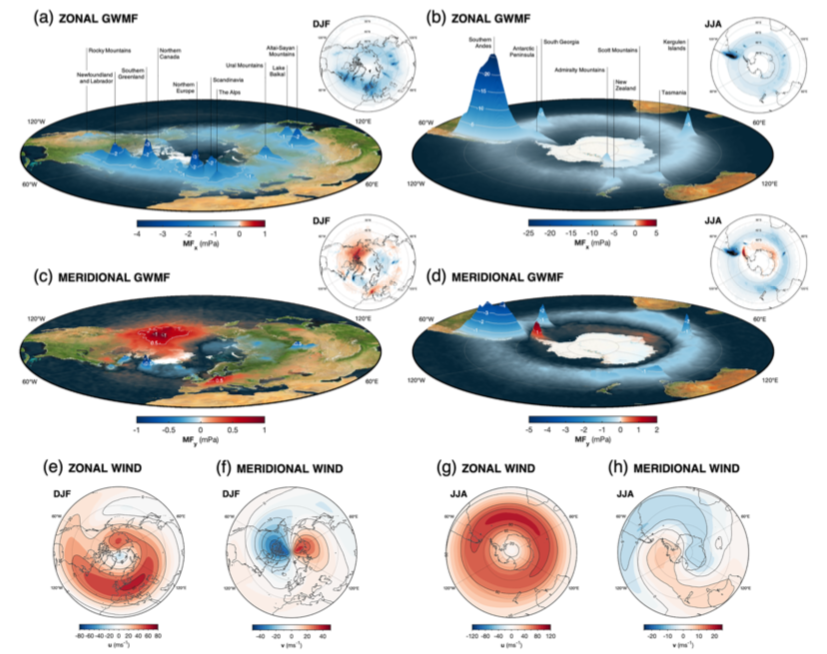
\includegraphics[width=0.99\textwidth]{Figures/hindley_2020_GWMF.png}
    \caption{Stereographic maps of average wintertime zonal (a, b) and meridional (c, d) GWMF near 40 km altitude derived from AIRS/Aqua 3‐D satellite observations for the period 2002–2019. Winter is defined as December–February (June–August) for the Northern (Southern) Hemisphere. GWMF values that are close to zero have been made transparent to reveal the surface features below, and landmarks that lie beneath regions of increased GWMF have been labeled. Inset in the top right of each panel is a stereographic map of the same data but centered on the north and south poles. These inset panels share a color scale with the corresponding 3‐D contours. Panels (e)–(h) show average wintertime zonal and meridional winds at 3 hPa for the period 2002–2019 from ERA5 reanalysis. Taken from \cite{hindley_18year_2020}.}
    \label{fig:hindley_2020_GWMF}
\end{figure*}
%
The increasing number of GW observations from satellites (\cite{hindley_gravity_2019}, \citeyear{hindley_18year_2020}), ground-based lidar systems (\cite{kaifler_lidar_2020} and  \cite{kaifler_compact_2021}), aircraft (\cite{rapp_southtrac-gw_2021} and \cite{fritts_deep_2016}) and  balloons (\cite{plougonven_gravity_2013}) help to constrain GW parameterisations, but also reveal their deficiencies and point out gaps in our current theoretical knowledge on GWs. A phenomenon that was already visible in observations by \textcite{wu_satellite_1996}, but still lacks a conclusive explanation, is a GW belt around 60 \degree S during the austral winter. It is visualized in parts b and d of Fig. \ref{fig:hindley_2020_GWMF} from \textcite{hindley_18year_2020} who provide an extensive overview on seasonally averaged multi-year gravity wave momentum flux (GWMF) derived from satellite observations.


Orography undoubtedly leads to the GW hot spot between $55 \degree$W and $80 \degree$W above the southern Andes and the Antarctic Peninsula,  but it only contributes about $25 \%$ to the total GWMF within the latitude band from $35 \degree$S to $68 \degree$S as stated by \textcite{hindley_18year_2020}. Following \textcite{sato_gravity_2012} and accounting for a far downstream propagation of GWs excited by the Andes, the observable GWMF in the East of the defined longitude region could be allocated to this predominantly local source, too. However, this does not heavily affect the argument of \textcite{hindley_18year_2020} that about $75 \%$ of zonal and meridional GWMF are observed at remaining longitudes over the Southern Ocean mostly peaking around $60 \degree$S (\cite{hindley_18year_2020}).

It has been shown that small, mountainous islands contribute to this oceanic GWMF (\cite{garfinkel_effect_2018}; \cite{mclandress_is_2012}, \cite{alexander_momentum_2009}), but again they only result in local peaks as indicated in Fig. \ref{fig:hindley_2020_GWMF}b. So non-orographic origins of GWs are most likely the reason for the wide-spread, belt-like structure of the GWMF (\cite{hendricks_what_2014}). Jet streams and fronts most likely contribute to the observed momentum flux (\cite{plougonven_internal_2014} and \cite{hendricks_what_2014}) and have also been investigated on the basis of idealized simulations (\cite{osullivan_generation_1995}). \textcite{polichtchouk_sensitivity_2018} analysed the sensitivity of high-resolution atmospheric models to non-orographic GW parameterisations and concluded a significant dependence in the same manner as \textcite{choi_effects_2013} showed that convective gravity wave drag parameterisations (a specific non-orographic source) can have a significant influence on global climate models. In addition, \textcite{jewtoukoff_comparison_2015} were able to assign wave signatures in their balloon observations to non-orographic sources, but so far none of the discussed mechanisms provides a comprehensive explanation of the wide spread observation of GWs over the Southern Ocean in the austral winter and it is still possible that some important mechanisms have not yet been considered.

The gravity wave belt around 60$\degree$S gained crucial relevance since \textcite{mclandress_is_2012} suggested its connection to the longstanding cold pole problem found in nearly all modern GCMs and chemistry climate models (CCMs). During the southern hemisphere winter months a polar vortex or polar night jet (PNJ) develops around 60$\degree$S high up in the stratosphere characterized by strong zonal westerly winds. GCMs and CCMs overestimate this PNJ, which also entails lower stratospheric temperatures over the pole compared to observations (\cite{butchart_multimodel_2011}, \cite{geller_comparison_2013} and \cite{eyring_sparc_2010}). As a result, the polar vortex breaks down too late in the spring with significant consequences on, for example, the simulated ozone trends in the Antarctic middle stratosphere (\cite{stolarski_ozone_2006}). The Antarctic ozone hole persists too long into the late spring and since Antarctic ozone depletion is the primary driver of recent southern hemisphere summertime climate change (e.g. \cite{arblaster_contributions_2006}), a delay in the vortex breakdown impacts the timing of the simulated tropospheric response.

\textcite{mclandress_is_2012} showed through their simulations that missing gravity wave drag from parameterisations can explain this substantial zonal wind bias around 60°S and the directly related "cold pole". A deeper understanding of the key processes that lead to the observed gravity wave belt during the austral winter could significantly improve GW parameterisations and ultimately improve long-term climate predictions through more realistic and robust GCMs. 

% include polar vortex image to show zonal wind distribution.

% or if it ultimately is a superposition of all known sources.

% temperature measurements of satellite
% in the vicinity of the 60°S belt

%%%
% excitation, propagation and dissipation
% \textcite{}
% \citeyear{}
%%%

\section{The excitation of GWs above tropopause depressions}
\label{sec:excitation}

As outlined in the previous section, non-orographic GW sources have already been investigated from various perspectives, but are not yet able to fully explain the consistent, wide-spread appearance of GWs around 60$\degree$S. Based on observations and the analysis of high-resolution ERA5 data, \textcite{dornbrack_stratospheric_2022} are currently proposing a new mechanism that has the potential to fill this gap. They suggest the excitation of GWs above tropopause depressions (TDs) in the stratosphere just like they would appear above surface obstacles in the troposphere. 

Though various definitions of the tropopause exist, all rely on abrupt changes in physical or chemical properties when transitioning from a weakly stratified troposphere ($N^2 \approx$ 1$\cdot 10^{-4}$\SI{}{s^{-2}}) to a comparatively strongly stratified stratosphere ($N^2 \approx$ 4$\cdot 10^{-4}$\SI{}{s^{-2}}; \cite{birner_fine-scale_2006}). Common definitions are based on the thermal stratification (negative temperature lapse rate in the troposphere, positive  lapse rate in the stratosphere; \cite{wmo_meteorology_1957}), refer to the dynamical tropopause using Ertel's potential vorticity (\cite{wmo_atmospheric_1986}) or rely on chemical tracers like ozone. Despite fundamental differences in those approaches, each supports the simplification of treating the tropopause as an impermeable boundary, which is definitely not true, but a good approximation for idealized investigations. 

In the vicinity of jet streams or upper level frontal zones and associated with baroclinic processes the extratropical tropopause now  experiences deflections or even undergoes a folding process as visualized in Fig. \ref{fig:skerlakFold}. Dry stratospheric air penetrates down into the troposphere and folds underneath the warm air towards the equator (here northward for southern hemisphere) for deep depressions. % Potentially warmer stratospheric air
%
\begin{figure*}[ht]
    \centering
    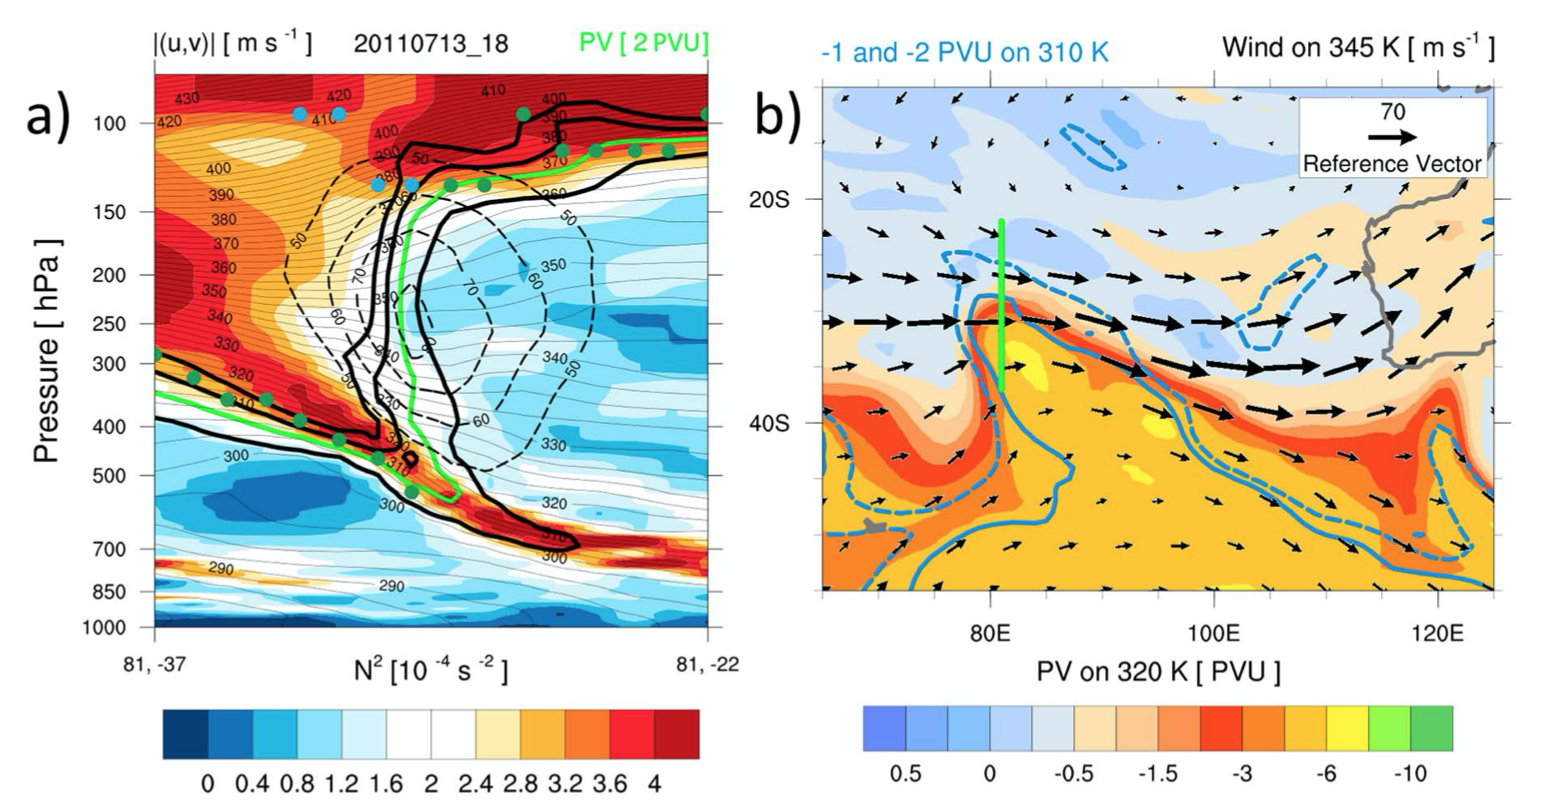
\includegraphics[width=0.99\textwidth]{Figures/Skerlak_Fold.png}
    \caption{Example of a deep tropopause fold near the subtropical jet west of Australia at 18 UTC on 13 July 2011. The vertical cross section shown in Figure 2a is aligned along 81$\degree$E from 37S$\degree$ to 22$\degree$S (green line segment in Figure 2b). Displayed are (a) the squared Brunt-Vaisala frequency ($N^2$, colored), potential vorticity (-1 to -4 PVU, thick solid lines, -2 PVU in green, rest in black), the WMO first and second tropopauses (green and blue solid circles, respectively), horizontal wind speed (in \SI{1}{\meter\second^{-1}}, dashed contours), and isentropes (in K, thin contours) and (b) PV on 320 K (colored, in PVU), contours of PV on 310 K at -1 PVU and -2 PVU (dashed and solid blue, respectively), and horizontal wind speed on 345K (reference vector in the top right, in \SI{1}{\meter\second^{-1}}). The West Coast of Australia is visible as grey contour. Taken from \cite{skerlak_tropopause_2015}.}
    \label{fig:skerlakFold}
\end{figure*}
%
The shape of the TD and especially the vertical extend of the prominent tongue of stratospheric air can vary significantly depending on the large scale flow conditions and strength of the upper level frontal system. This has already been discussed extensively from an observational (e.g. \cite{shapiro_further_1978} and \cite{keyser_review_1986}) and model (\cite{skerlak_tropopause_2015}) perspective. Fortunately, the excitation of GWs above such a depression might not be very sensitive to the fold's shape far below the tropopause. Isentropes, that are deflected downwards, but rise again on the other side of the depression (e.g. 360-\SI{390}{\kelvin} in Fig. \ref{fig:skerlakFold}a) are much more interesting for the proposed mechanism considering its similarity to flow over orography. Additionally, the zonal shape of the depression is more relevant for the GW forcing. This along-stream cross section (orthogonal on \ref{fig:skerlakFold}a) was rarely discussed in relevant publications, since the main folding process happens in the cross-stream direction. Based on the ERA5 case study conducted by \textcite{dornbrack_stratospheric_2022} (Fig. \ref{fig:RF25_waves}), the zonal width at half maximum of the propagating TD can be estimated between $4 \degree$ and $8 \degree$ in zonal direction, which transfers to $a=240-$\SI{480}{\kilo\meter}
($1\degree \approx$ \SI{63}{\kilo\meter} at $55 \degree$S). 

% Significant intrusions of stratospheric air occur in “ribbons” ~200 to 100 km in length, 100 to 300 km wide and about 1 to 4 km thick (EPA 2006).


Following estimates based on idealized scenarios (constant background wind $U$ and Brunt–Väisälä frequency $N$) such 'mountain widths' are expected to excite waves within the hydrostatic regime. Towards the wider end of $a$ the advection time for an air parcel to pass over the mountain $\tau_a = \frac{a}{U}$ is even comparable in magnitude to the period of inertial oscillation due to Earth’s rotation ($\tau_f = \frac{2 \pi}{f}$) with the Coriolis parameter $f \approx 10^{-4}$\SI{}{\second^{-1}} for mid-latitudes. So the Rossby number
% Thus, the time it takes for a fluid particle to cross the ridge is much larger than the period of a buoyancy oscillation
% We notice that τf /τa = 2πU/(fa) ≈ Ro
\begin{equation}
    Ro = \frac{U}{f a} \approx \frac{\tau_f}{\tau_a} \approx 2 \pi
\end{equation}
%
is close to $O(1)$ and Coriolis forces can no longer be neglected. Together with the buoyancy forces they act together as restoring forces resulting in both horizontal and vertical oscillations, which are called hydrostatic inertia-gravity waves (e.g. \cite{gill_atmosphere-ocean_1982} and \cite{lin_mesoscale_2007}).
% Froude number for linear non-linearity with height!!
% $L N U^{-1}$
% should be 60 m/s wind or 100km wide depression for hydrostatic scenario

A major difference of potential GWs above TDs to classic mountain waves is the transient nature of their source. \textcite{pfister_gravity_1993} already investigated the propagation of waves in the stratosphere due to a transient forcing by exposing the background flow to a time-varying obstacle, but only lifted and receded the bottom of the stratosphere. A tropopause fold travels eastward with the phase speed of the Rossby wave, so the relative motion of the stratospheric air aloft with respect to the propagation of the fold is responsible for the excitation of the GWs. The increasing wind speed with height due to the PNJ, which is already important for the propagation of the waves, is, therefore, important for their excitation, too.

\section{The propagation of GWs above tropopause depressions}
\label{sec:propagation}

Considering the hydrostatic nature of GWs excited by TDs, the strongest wave signal should more or less appear directly above a propagating depression. In fact, \textcite{dornbrack_stratospheric_2022} observed exactly this feature in ERA5 data (Fig. \ref{fig:RF25_waves}), when analysing lidar measurements from DEEPWAVE research flight 25. Clear wave signals are observed directly above the tropopause fold for multiple points in time. This inspires confidence in the proposed mechanism and suggests that GWs can be observed along the whole path of the baroclinic system responsible for the depression.
%
\begin{figure*}[ht]
    \centering
    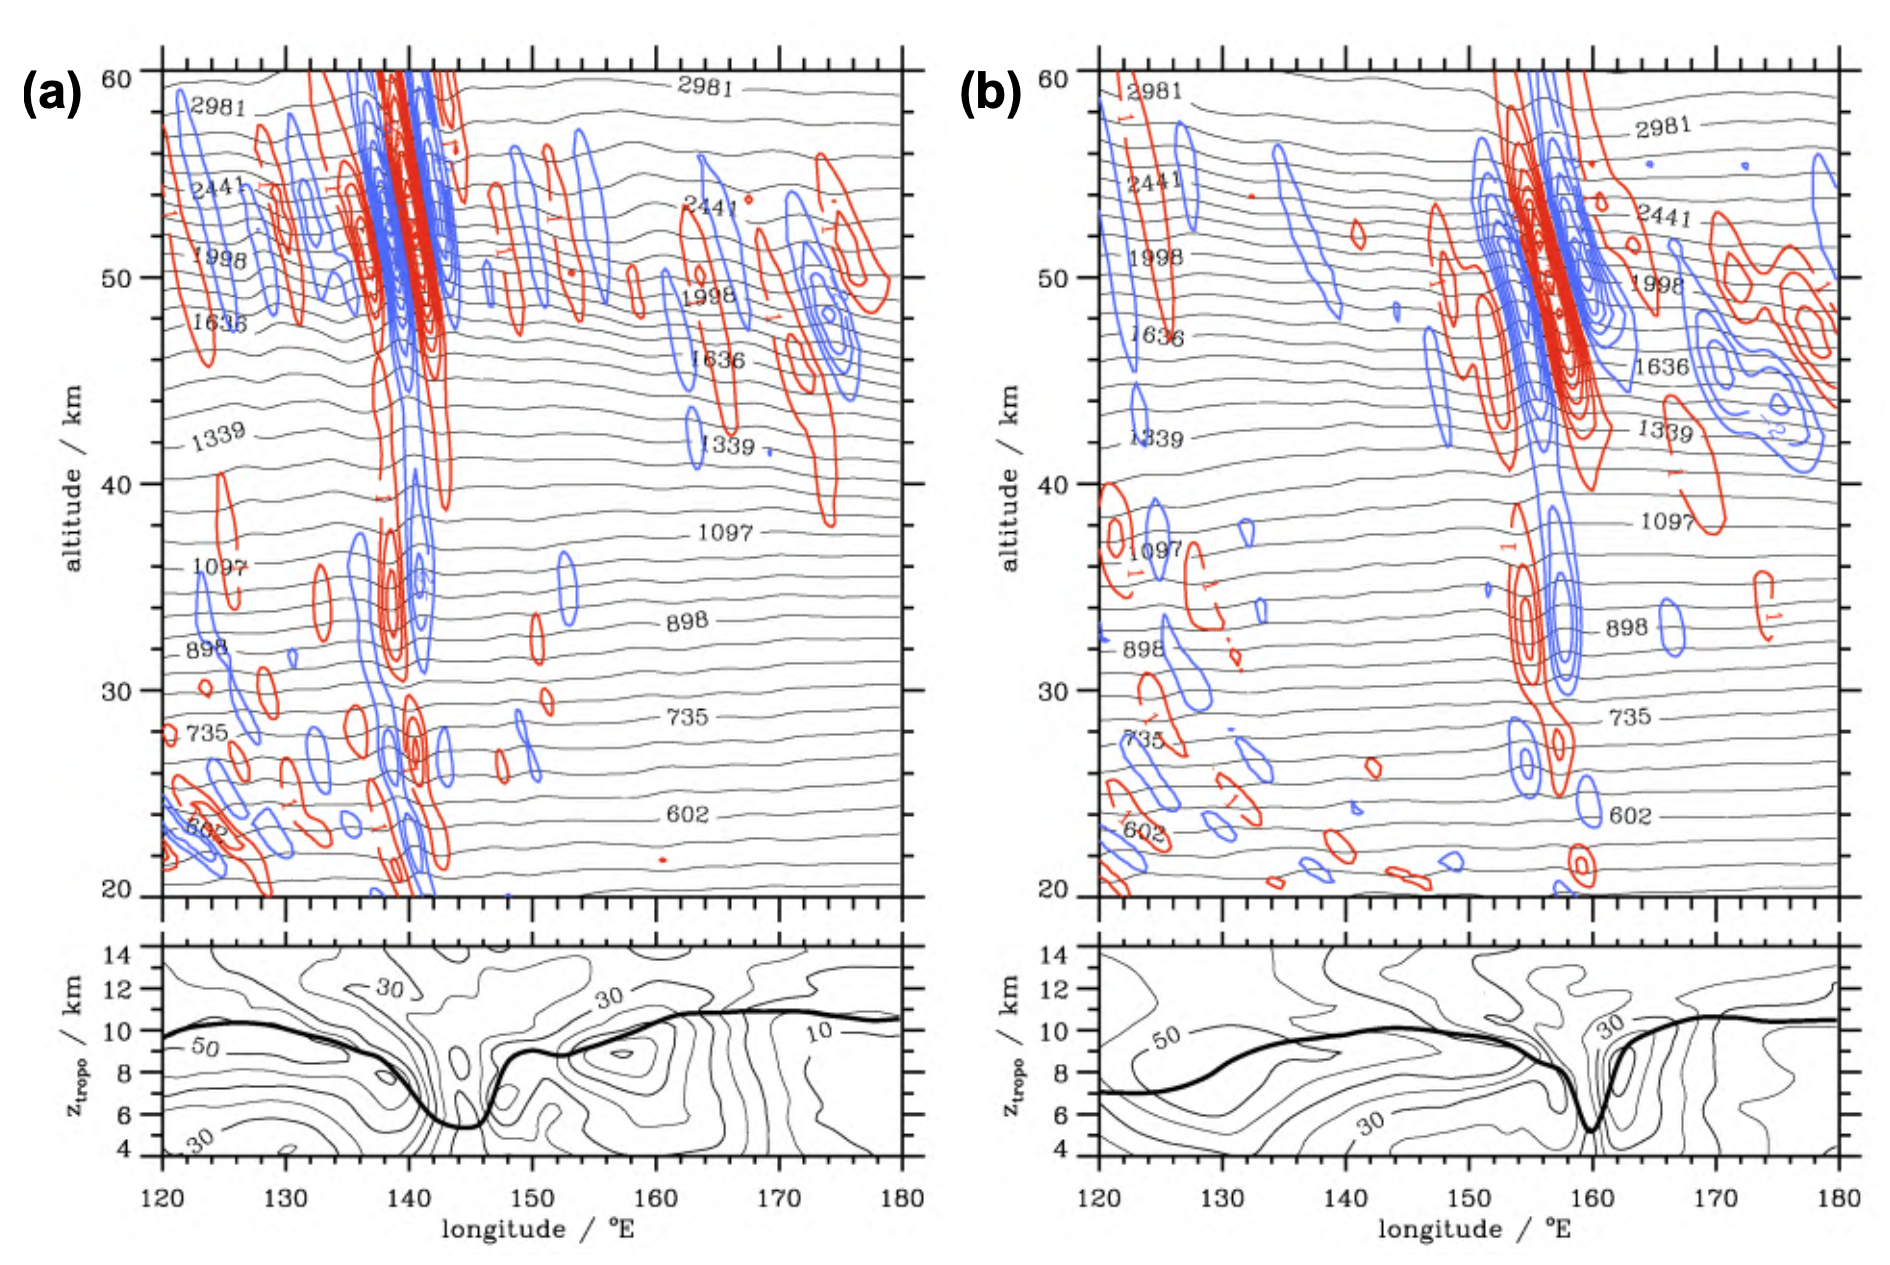
\includegraphics[width=0.99\textwidth]{Figures/RF25_waves.png}
    \caption{Temperature perturbations (K, red and blue contour lines) and potential temperature (K, black lines in logarithmic scaling) along 55$\degree$S on 17 July 2014 15 UTC (a) and 18 July 2014 09 UTC (b). The bottom panels depict the height of the dynamical tropopause (thick black lines, meridional average from 52.5$\degree$S to 57.5$\degree$S) and the horizontal wind (\SI{}{\meter\second^{-1}}, thin black lines) at the same instances. Data: One hourly ERA5 data. Taken from Dörnbrack et al. (2021).}
    \label{fig:RF25_waves}
\end{figure*}
%
Now, the last piece to the puzzle for explaining the wave belt above the Southern Ocean during the austral winter in Fig. \ref{fig:hindley_2020_GWMF}b and \ref{fig:hindley_2020_GWMF}d is the meridional propagation of GWs in the stratosphere. This is important, because especially in the southern hemisphere pronounced frontal systems are not deviating significantly from a latitude band around 50$\degree$S (\cite{skerlak_tropopause_2015}) though GWs are observed frequently further south.

Two mechanisms are at hand concerning this meridional propagation. At first, the orientation of the TDs is rarely exactly North-South resulting in an inclined wave vector with respect to the predominantly westerly flow in the upper stratosphere. The wave vector defines the propagation direction, so this mechanism is always present and relevant as soon as tilted obstacles are in place as discussed by \textcite{preusse_space-based_2002} for GWs excited by the Andes at similar latitudes. The second process is based on ray-tracing theory and was first discussed and applied by \textcite{dunkerton_dunkerton_inertiagravity_1984}. It describes the modification of the meridional (horizontal) wavenumber by the background wind field with
%
\begin{equation}
    \frac{dl}{dt} = -(k \frac{\partial U}{\partial y} + l \frac{\partial V}{\partial y} + \frac{\beta f}{\hat{\omega}})
    \approx -k \frac{\partial U}{\partial y}.
    \label{equ:meridionalRefraction}
\end{equation}
%
In a simplified scenario the time rate of change of the meridional wavenumber $l$ along the ray is proportional to the meridional gradient of the background wind $U$ and the zonal wavenumber $k$. In other words, horizontal wind shear develops a meridional component of the wave vector even in the case of a purely zonal initial propagation. In general, this phenomenon leads to a refraction of internal GWs into the southern hemispheric PNJ at 60$\degree$S, which has already been described by a number of publications (e.g. \cite{dunkerton_dunkerton_inertiagravity_1984}, \cite{preusse_space-based_2002}, \cite{sato_origins_2009}, \cite{sato_gravity_2012}, \cite{ehard_horizontal_2017} and \cite{jiang_stratospheric_2019}). \textcite{jiang_stratospheric_2019} further add, that waves are elongated towards the stronger background wind (towards the center of the PNJ) and shortened on the opposite side with weaker winds.

\section{Research goals and outline}
\label{sec:goals}
%
In the end, both described mechanisms play an important role for the meridional propagation of GWs. Together with the regular appearance of Rossby wave trains (baroclinic systems involving TDs) at middle latitudes in the southern hemisphere, these processes could provide a conclusive explanation for the widespread and patchy stratospheric GW activity all the way around the Southern Ocean shown in Fig. \ref{fig:hindley_2020_GWMF}b and \ref{fig:hindley_2020_GWMF}d. It is the goal of the proposed thesis to further investigate the relevant processes related to GWs above tropopause depressions through idealized simulations and eventually provide first answers on its relevance for explaining the discussed GW belt above the Southern Ocean. More specifically, the Master's thesis shall answer the following research questions:
%

INCLUDE OUTLOOK OF andreas paper with suggestions for further work

\begin{enumerate}
    \item How sensitive is the excitation and propagation of GWs above TDs to the shape of the depression (depth, width, asymmetry)?
    \item Which wave regimes are present above propagating TDs and what wavelengths and amplitudes do we expect?
    \item What is the contribution of a tilted TD (leading to an inclined wave vector) to a meridional propagation of GWs?
    \item What is the contribution of horizontal wind shear in the stratosphere to a meridional propagation of GWs?
    % \item How significant is the effect of the Coriolis force in 2D and 3D simulations?
\end{enumerate}

%% In baroclinic simulation advection of waves meridionally possible!!!

% Stationary synoptic patterns like blocks are rare in the southern hemisphere, because of 

%% NOTES %%
% include figure and description
% hydrostatic waves (include figure from RF25 of waves above depression)

% It is clear that the flow regime above a TD is much more complicated than a zonal overflow of an elongated mountain ridge, which produces the expected hydrostatic waves aloft. Three dimensional Furthermore, the fold itself travels eastward with the phase speed of the Rossby

% impermeable boundary
% shear wind rotation with height to strong zonal wind 

% The World Meteorological Organization defines the tropopause as the lowest level where the abso- lute value of the temperature lapse rate decreases to 2K/km. or less, with the average lapse rate between this level and all higher levels within 1.2 mi. (2 km.) not exceeding 2K/km. The dynamical tropopause is defined in terms of sharp changes in the potential vor- ticity (much higher in the stratosphere), which mea- sures stratification and rotation of the air masses. An abrupt increase (decrease) with height of the ozone (water vapor) mixing ratio indicates the presence of the chemical tropopause.

% thermal definition
% dynamic definition potential temperature and pressure on the dynamic tropopause (defined here as the 1.5 × 10−6 m2 K kg−1 s−1, hereafter 1.5 PVU, Ertel PV surface)
% chemical definition

% thermal fields and wind fields

% bush vertical / horizontal aspect ratio of 0.06 penetrates the troposphere

% \cite{clark_convectively_1986} above inversion layer?? 
\newpage
\thispagestyle{plain}

% ==== CHAPTER 2 ===============================================================
% ---- set some counters to zero:
\setcounter{equation}{0}
\setcounter{table}{0}
\setcounter{figure}{0}
% ---- include tex-file:
\chapter{Methods and data}

The following subsections provide a sufficient overview on the numerical model and analysis tools used for the presented work to allow a conclusive interpretation of the results thereafter.

%%%%% EULAG %%%%%

\section{CORAL temperature measurements} 
\label{sec:coral}

\textcite{kaifler_compact_2021} provide a more extensive summary on CORAL's setup and observation,


\section{(ERA5 reanalysis data)}



\section{Spectral filtering}
% FFT

refer to filtering described in Kruse paper and from Vera
but mention equations


and describe butterworth filter for CORAL data

\section{Wavelet Analysis}


% Mithilfe der Wavelet-Transformation können aus einer Datenreihe nicht nur die auftre- tenden Frequenzen extrahiert werden, sondern auch Informationen darüber, in welchen Abschnitten der Datenreihe welche Frequenzen dominant sind. Als Basisfunktionen wer- den dabei räumlich lokalisierte Wellen, sogenannte Wavelets, verwendet.

% Folgenden wird die Wavelet-Analyse anhand einer Datenreihe f(z) erläutert, die ent- lang einer räumlichen Achse z variiert. Dabei wird auf die Beschreibung in Torrence & Compo (1998) zurück gegriffen. Die Autoren stellen auf der Website http://atoc.colorado.edu/research/wavelets/ Software zur Anwendung der Wavelet-Ana- lyse zur Verfügung, die in dieser Arbeit verwendet wurde.
% Hier wurde das Morlet-Wavelet ψ0(η) benutzt, das von einem dimensionslosen Ortspa- rameter η abhängt und als
% ψ0(η) = π−1/4 ei ω0η e−η2/2 (3.39)
% definiert ist. Real- und Imaginärteil von ψ0 sind in Abbildung 3.6a dargestellt. Wird f(z) als eine Datenreihe fj diskretisiert, die bei konstanter Intervallgröße ∆z auf einem Gitter mit Index j = 0,...,N−1 definiert ist, kann daraus die kontinuierliche Wavelet- Transformation Wn(s) ermittelt werden. Diese ist definiert als Faltung von fj mit einer skalierten und verschobenen Version der Wavelet-Funktion:
% N−1 Wj(s) = �� fj′ ψ∗
% ��(j′ −j)∆z�� s
% (3.40) die komplex konjugierte normierte Wavelet-Funktion ψ0.
%  Hierbei ist ψ
% ∗
% ���� ∆z ��1/2 ��∗ = s ψ0
% j′=0
%  Indem die Wavelet-Skala s variiert und ψ∗ entlang des Ortsindex j verschoben wird, kann ein Bild rekonstruiert werden, das sowohl die Amplitude einzelner Merkmale des Signals zeigt als auch die Variation der Amplitude mit dem Ort.
% Für jede Skala s muss Gleichung (3.40) N-mal angewandt werden, damit die kontinu- ierliche Wavelet-Transformation approximiert wird. Diese Berechnung erfolgt deutlich schneller im Fourier-Raum, wo die Wavelet-Transformation gleichzeitig für alle N durch- geführt werden kann. Für die Skalen s empfiehlt sich eine Wahl von M Skalen, die als Vielfache von 2 ausgedrückt werden:
% sm = s0 2m∆m mit m = 0,1,...,M und M = ∆m−1 log2(N ∆m/s0)
% Die kleinste Skala s0 sollte dabei so gewählt werden, dass die entsprechende Fourier-
% Periode etwa 2∆z beträgt. Aus der komplexen Wavelet-Transformierten Wj(s) kann
% das reelle Wavelet-Leistungsspektrum |Wj(s)| berechnet werden. Bei der Interpretation
% dieses Spektrums muss beachtet werden, dass bei der Fourier-Transformation eine An-
% nahme bezüglich zyklischer Daten gemacht wird, die nicht unbedingt erfüllt ist. An den
% Rändern des Datensatzes können deshalb Fehler auftreten. Der Einflusskegel (engl.: cone
% of influence) gibt an, in welchen Bereichen des Spektrums Randeffekte wichtig werden.
% Er ist definiert als e-Abklingzeit τs der Wavelet-Leistung zu jeder Skala s und für das √
% Morlet-Wavelet gilt τs = 2 s.
% Im rechten Bildteil von Abbildung 3.6c ist ein Wavelet-Leistungsspektrum dargestellt, in dem auch der Einflusskegel als weiße Linie markiert ist. Die schwarze Kontur gibt ein Konfidenzniveau von 95 % an, bezogen auf ein Spektrum roten Rauschens mit lag-

% 1-Koeffizient 0.72 (siehe Torrence & Compo, 1998). Es zeigt die Wavelet-Analyse ei- nes Profils des Vertikalwinds (mittlerer Bildteil von Abbildung 3.6c) aus einer EU- LAG-Simulation. Der Vertikalschnitt durch das Windfeld ist in Abbildung 3.6b als rot-gestrichelte Linie dargestellt. Im Wavelet-Leistungsspektrum, das mit dem Morlet- Wavelet (Abbildung 3.6a) erstellt wurde, können einzelne Bereiche als dominante Signale ausgemacht werden. Im unteren Bereich bis zu einer Höhe von z = 10 km ist eine ver- tikale Wellenlänge λz zwischen etwa 2 000 m und 3 000 m verstärkt vorhanden, während in größeren Höhen kleinere Wellenlängen von unter 1000m das Spektrum bestimmen. Dieser Fall ist in Abschnitt 4.2.1 ausführlich besprochen.


% include figure from wavelet analysis for one line in 2D data, show line in T' plot..

% Figure: wavelet + cut + power spectrum 

spectral resolution was \cite{torrence_practical_1998}
\newpage
\thispagestyle{plain}

% ==== CHAPTER 3 ===============================================================
% ---- set some counters to zero:
\setcounter{equation}{0}
\setcounter{table}{0}
\setcounter{figure}{0}
% ---- include tex-file:
\chapter{The numerical model EULAG}

Refer to work of Grogger that investigated deep propagating GWs, individual spectral forcings, linear analysis vs numerical results...

Grogger also showed EULAG simulations for transient lower boundary, more specifically growing amplitude / rising topography 

extend with the comparing numerical to analytical results of GWD for different MW regimes...
and show transient lower boundary moving in x-direction

\section{General setup}
\label{sec:EULAG}

The nonlinear numerical simulations are conducted with the EUlerian/semi- LAGrangian fluid solver (EULAG). The model is set up solving the soundproof anelastic set of equations (\cite{lipps_scale_1982}) consisting of the three components of the momentum equation (\ref{equ:momEqu}), the thermodynamic equation (\ref{equ:potTemp}) for the potential temperature perturbation $\theta$'=$\theta-\theta_e$ and the mass continuity equation (\ref{equ:continuityEqu}):
%
\begin{equation}
\begin{aligned}
    \frac{d \Vec{v}}{dt} = -G \Vec{\nabla} (\frac{p'}{\bar{\rho}}) +  \Vec{g} \frac{\theta'}{\bar{\theta}} - 2 \Vec{\Omega} \times (\Vec{v}-\Vec{v_e}) \\
    - \Tilde{\alpha} (\Vec{v}-\Vec{v_e}) \equiv R^{v},
    \label{equ:momEqu}
\end{aligned}
\end{equation}
%
\begin{equation}
    \frac{d \theta'}{dt} = -\Vec{v} \cdot \Vec{\nabla} \theta_e - \Tilde{\beta} (\theta-\theta_e) \equiv R^{\theta},
    \label{equ:potTemp}
\end{equation}
%
\begin{equation}
    \Vec{\nabla} \cdot (\bar{\rho} \Vec{v}) = 0.
    \label{equ:continuityEqu}
\end{equation}
%
Here, $\frac{d}{dt}$, $\Vec{\nabla}$ and $\Vec{\nabla} \cdot$ represent the total derivative, the gradient and the divergence respectively. $p'$ is the pressure perturbation with respect to the environmental state, g the gravitational acceleration and $\Vec{\Omega}$ the angular velocity of the Earth. The matrix G represents geometric terms, which result from the general, time-dependent coordinate transformation and the symbol $R^{\Psi}$ stands for the right-hand side of the corresponding equations for the variables $\Psi = (u,v,w,\theta')$.
%
\begin{equation}
    \bar{\theta}(z) = \theta_0 \textrm{ exp}(-\frac{N^2}{g} z) 
    \label{equ:thetaScale}
\end{equation}
%
and the anelastic density 
%
\begin{equation}
    \bar{\rho}(z) = \rho_0 \textrm{ exp}(-\frac{z}{H_{\rho}})
    \label{equ:densityScale}
\end{equation}
% with $H_{/rho} = 7314m$. 
refer to the hydrostatic reference state around a constant stability profile as introduced by \textcite{bacmeister_breakdown_1989} with stability $\frac{N^2}{g}$, a density scale height $H_{\rho}$ that corresponds to a deep atmosphere and $\rho_0$, $\theta_0$ set to appropriate reference constants. With (\ref{equ:thetaScale}) and (\ref{equ:densityScale}) being the basic state of equations (\ref{equ:momEqu}-\ref{equ:continuityEqu}), a more general environmental state, which reflects the initial and boundary conditions, enters the equations via the variables with subscript e. In that sense, $\alpha(\Vec{v}-\Vec{v_e})$ and $\beta(\theta-\theta_e)$ represent relaxation terms, which enable the radiation of wave energy across the model boundaries and force the solutions at the model boundaries to the prescribed environmental profiles. These ambient states like $u_e$, $\rho_e$ or $\theta_e$ can be time-dependent to replicate transient flow conditions, but are stationary within the scope of this thesis. On the other hand, transient boundaries like a propagating tropopause fold almost demand for time-dependent terrain-following vertical coordinates as introduced by \textcite{wedi_extending_2003}, so this option may be considered at a later stage. Furthermore, EULAG is noteworthy for its robust elliptic solver (\cite{smolarkiewicz_forward--time_1993}) and generalized coordinate formulation enabling grid adaptivity technology (\cite{prusa_eulag_2008}, \cite{kuhnlein_modelling_2012}).

As the name suggests, EULAG is capable of solving the equations of motion (\ref{equ:momEqu}-\ref{equ:continuityEqu}) in an Eulerian (flux form) or in a semi-Lagrangian (advective form) mode (\cite{smolarkiewicz_forward--time_1997}). For the numerical approximation it utilizes a non-oscillatory forward-in-time (NFT) approach compactly formulated as
%
\begin{equation}
\begin{aligned}
    \Psi^{n+1} = LE(\Tilde{\Psi}, V^{n+1}, G^n, G^{n+1}) \\
    + \frac{1}{2} \Delta t R^{\Psi} |^{n+1}
    \label{equ:NFTscheme}
\end{aligned}
\end{equation}
%
with $LE$ representing the corresponding semi-Lagrangian/Eulerian transport operator. The NFT scheme belongs to the class of second-order-accurate two-time-level algorithms that are build on nonlinear advection techniques (\cite{prusa_eulag_2008}). These schemes have the property to suppress and control numerical oscillations that are often found in higher order linear schemes. As a result, transporting the auxiliary field $\Tilde{\Psi} = \Psi^n + \frac{1}{2} \Delta t R^{\Psi}|^n$ instead of the specific variable $\Psi$, results from a thorough truncation error analysis and ensures second order accuracy. (\cite{smolarkiewicz_forward--time_1997}).

Within the scope of this Master's thesis all simulations utilize the Eulerian option by applying the multidimensional positive definite advection transport algorithm MPDATA (\cite{smolarkiewicz_mpdata_1998} and  and \cite{smolarkiewicz_multidimensional_2006}).

EULAG has a proven itself as a reliable tool for simulating thermo-fluid flows across the wide range from turbulent to global scales (\cite{prusa_all-scale_2003}) and in a variety of of physical scenarios like e.g. turbulence, GW dynamics, flows past complex/moving boundaries, micrometeorology or cloud microphysics (\cite{prusa_eulag_2008}). A comparison between different well-established numerical models (including EULAG) and their capability to model flow over steep terrain, which is relevant for the investigations within this thesis, appears in \textcite{doyle_intercomparison_2011}.

%%%%% NOTES %%%%%
% Prusa 2008 also has good description of perturbation form and points out importance of correct environmental/initial state!! 

% \cite{smolarkiewicz_multidimensional_2006}

% \begin{equation}
%    \frac{\partial G \rho \Psi}{\partial t} + \nabla \cdot G \rho \Vec{v} = G \rho R
%    \label{equ:statMeshAdapt}
% \end{equation}


% he elliptic pressure equation is solved via a preconditioned non-symmetric Krylov sub- space solver (Smolarkiewicz and Margolin; 1994; 1997, Skamarock et al., 1997).

% imlicit /explicit elliptic pressure solver / krylov sub space solver

% There, governing equations are formulated in general- ized time-dependent curvi-linear coordinates to enable mesh adaptivity (Prusa and Smolarkiewicz 2003; Wedi and Smolarkiewicz 2004; Kühnlein et al. 2012; Smolarkiewicz and Charbonneau 2013) and continuous mappings of the Earth’s topography by using terrain-following coordinates (Gal-Chen and Somerville 1975; Clark 1977)


% anelastic -> elastic energy is not allowed -> sound waves are filtered since they are based on pressure difference rather then temperature


\section{Ambient profiles of idealized simulations}
% mark variables to be defined in table!! like in isentropic paper lightcyan
profile of potential temperature (definition of N) sets up background profiles


choice of kappa is not relevant for simulations with using the soundproof anelastic equations similar to \textcite[]{lipps_scale_1982}. The correct value for diatomic gases is $\kappa=\frac{2}{7}$. For simulations of the stratosphere with N=0.02 This leads to a reasonable temperature of 239K, but for N=0.01, a reasonable value for the troposphere, ambient profiles following \textcite{bacmeister_breakdown_1989} would result in T=900k. Therefore, T = 290K... with K=


EULAG provides multiple options to define background states of the atmosphere. For the presented simulations vertical ambient profiles define an isothermal atmosphere with constant stability as described by \textcite{bacmeister_breakdown_1989}. These exponential profiles of potential temperature and density avoid physical restrictions towards higher altitudes and are thus well suited for the investigation of deep gravity wave propagation. Defining a potential temperature and density scale height $H_{\Theta}$ and $H_{\rho}$ leads to


\begin{equation}
    \bar{\theta}(z) = \theta_0 \textrm{ exp}(-\frac{N^2}{g} z) 
    \label{equ:thetaScale}
\end{equation}
%
and the anelastic density 
%
\begin{equation}
    \bar{\rho}(z) = \rho_0 \textrm{ exp}(-\frac{z}{H_{\rho}})
    \label{equ:densityScale}
\end{equation}
% with $H_{/rho} = 7314m$. 
refer to the hydrostatic reference state around a constant stability profile as introduced by \textcite{bacmeister_breakdown_1989} with stability $\frac{N^2}{g}$, a density scale height $H_{\rho}$ that corresponds to a deep atmosphere and $\rho_0$, $\theta_0$ set to appropriate reference constants.

\begin{equation}
\begin{aligned}
    p_0(z) &= p_{00} e^{-\frac{z}{H_{\rho}}} \quad \textrm{with} \quad H_{\rho} = \frac{R_d}{c_p} H_{\Theta} = \frac{R_d T_{00}}{g} \\
    \rho_0(z) &= \frac{p_0(z)}{R_d T_{00}} = \rho_{00} e^{-\frac{z}{H_{\rho}}} \\
    T_0(z) &= \frac{p_{00}}{R_d \rho_{00}} \\
    \Theta_0(z) &= T_{00} \frac{p_{00}}{p}^{\kappa} \\
    \Theta_0(z) &= T_{00} e^{\frac{z}{H_{\Theta}}} \quad \textrm{with} \quad H_{\Theta} = \frac{g}{N^2} \\
    \label{equ:ambient-Profiles}
\end{aligned}
\end{equation}
% based on hydrostatic approximation dp/dz = -rho*g -> pressure with density scale height

with the Brunt-Vaisala frequency $N$, the specific gas constant $R_d$ and the specific heat capacity at constant pressure $c_p$. $p_0$, $\rho_0$ and $T_0$ represent a reference state of the atmosphere.

\begin{table*}[ht]
\centering
\caption{Parameters related to the ambient reference state and vertical profiles following \textcite[]{bacmeister_breakdown_1989}. Values for the troposphere are used for the model validation in section \ref{sec:linear-MWs}. Values for the stratosphere are used for the main simulations of this thesis described in chapters \ref{sec:resultsQ3D} and \ref{sec:results3D}. Colored cells refer to parameters that need to be defined.}

%%%% include trop for diatomic gas - then explain difference
%%% do scaled values still make sense
\begin{tabular}{@{}cccc@{}}
\toprule
 & Unit & Troposphere & Stratosphere \\ \midrule[1pt]

$R$ & J kg$^{-1}$ K$^{-1}$ &   \cellcolor{LightCyan} 287.04 &   \cellcolor{LightCyan} 287.04 \\
$g$ & m s$^{-2}$ & \cellcolor{LightCyan} 9.80616 & \cellcolor{LightCyan} 9.80616 \\
$N$ & s$^{-1}$ & \cellcolor{LightCyan} 0.01 & \cellcolor{LightCyan} 0.02 \\
$H_{\Theta}$ & m & 98061.6 & 24515.4  \\
$H_{\rho}$ & m & 28017.6 (8011.3)  & 7004.4 \\
$\kappa$ & - & $ \frac{2}{7}$ ($\frac{2}{24.4}$) & $ \frac{2}{7}$ \\
$c_p$ & J kg$^{-1}$ K$^{-1}$ & $\frac{7}{2} R$ ($\frac{24.4}{2} R$) & $\frac{7}{2} R$ \\

& & & \\
$T_{00}$ & K & \cellcolor{LightCyan} 957.17 (273.69) & 239.39 \\
$p_{00}$ & Pa &  \cellcolor{LightCyan} $1.01 \cdot 10^5$ & \cellcolor{LightCyan} $0.235 \cdot 10^5$ \\
$\rho_{00}$ & kg m$^{-3}$ & 0.3676 (1.2856) & 0.3454 \\

% kappa = H_rho/H_th 

\bottomrule
\end{tabular}
\label{tab:ambientProfiles}
\end{table*}

Should density scale height fit to reference state or should it rather relate correctly to stability / theta scale height based on two atomic gases? This results in temperature around 900K...
Value of density scale height effects

For stratosphere simulations it s fully consistent!!! 

- full 3D simulations (cite zhang.. 2005 together with Alexander/Durran...) extend those simulations to upper stratosphere.


\section{Transient lower boundary of idealized simulations}
% simulations without Coriolis in 2D

move and stop 


Describe cos function and derivative of lower boundary (similar as in papers)




show how wave propagate -> observe energy propagation / phase lines...


\section{Non-linear simulations of MW regimes with linear analytic solutions}
\label{sec:linear-MWs}
% for different MW regimes with non-linear numerical simulation}

% use small amplitude of 100m to avoid non-linear effect
% Show analysis plots for one simulation and then result of drag for all


% analysis of MFx, EFx, ... profiles for MW regime... thoughts on effect of CORIOLIS!!! MFx not constant...
% Witch of Agnesi mountain - no cos^4
One established approach to validate a numerical model is the comparison of non-linear numerical simulations to results from linear theory. For the investigation of GWs and corresponding processes drag values and momentum flux distributions are suitable.

% - \textcite{blumen} (Blumen 1965a, Fig. I)

- \textcite{bretherton_momentum_1969}

- \textcite{smith_influence_1979} looked circular bell-shaped mountain? only looks at 2D flow of stratified rotating fluid! Flow is independent of y coordinate! 

- Smith assumes symmetric mountain and only looks at one dimension in spectral space?? assumes geostrophic flow? uses gaussian quadrature or bessel functions...

- dimensionless drag is specified differently for Smith and miranda due to additional dimension

- \textcite{miranda_non-linear_1992} obtained the wave drag in a more general non-hydrostatic rotating case and derived an analytic solution for the hydrostatic rotating limit circular bell-shaped mountain. 

- integrate over two dimensions and assume a cross-section with V=0 to calculate drag. Keeps 3D problem first -> equations different to Smith, ...?

- W.K.B


\begin{table*}[ht]
\centering
\caption{Parameters for numerical simulations of different MW regimes: mountain width L, spatial increments $\Delta$x and $\Delta$z in the horizontal and vertical directions, time step $\Delta$t, thickness $\delta$x$_{ab}$ and time scale $\tau_x$ of the horizontal and altitude z$_{ab}$ and time scale $\tau_z$ of the vertical absorbers.}

\begin{tabular}{@{}cccccccc@{}}
\toprule
L/km & $\Delta$x/m & $\Delta$z/m & $\Delta$t/s & $\delta$x$_{ab}$/km & $\tau_x$/s  & z$_{ab}$/km & $\tau_z$/s \\ \midrule[1pt]

1   & 50  & 50 & 5   & 15  & 300  & 24 & 300   \\
2   & 100  & 50 & 5   & 30  & 600  & 24 & 450   \\
5   & 250  & 50 & 10  & 75  & 1200 & 24 & 600  \\
10  & 500 & 50 & 20  & 100 & 1800 & 24 & 900  \\
25  & 1000 & 50 & 40  & 200 & 3600 & 24 & 2400  \\
50  & 1500 & 50 & 60  & 300 & 4500 & 24 & 5400  \\
75  & 2000 & 50 & 60  & 400 & 6000 & 24 & 10500 \\
100 & 2500 & 50 & 75  & 500 & 7500 & 24 & 12000 \\
150 & 3500 & 50 & 180 & 700 & 9000 & 24 & 21000 \\

\bottomrule
\end{tabular}
\label{tab:linearRegimes}
\end{table*}


\begin{figure*}[tbp]
    \centering
    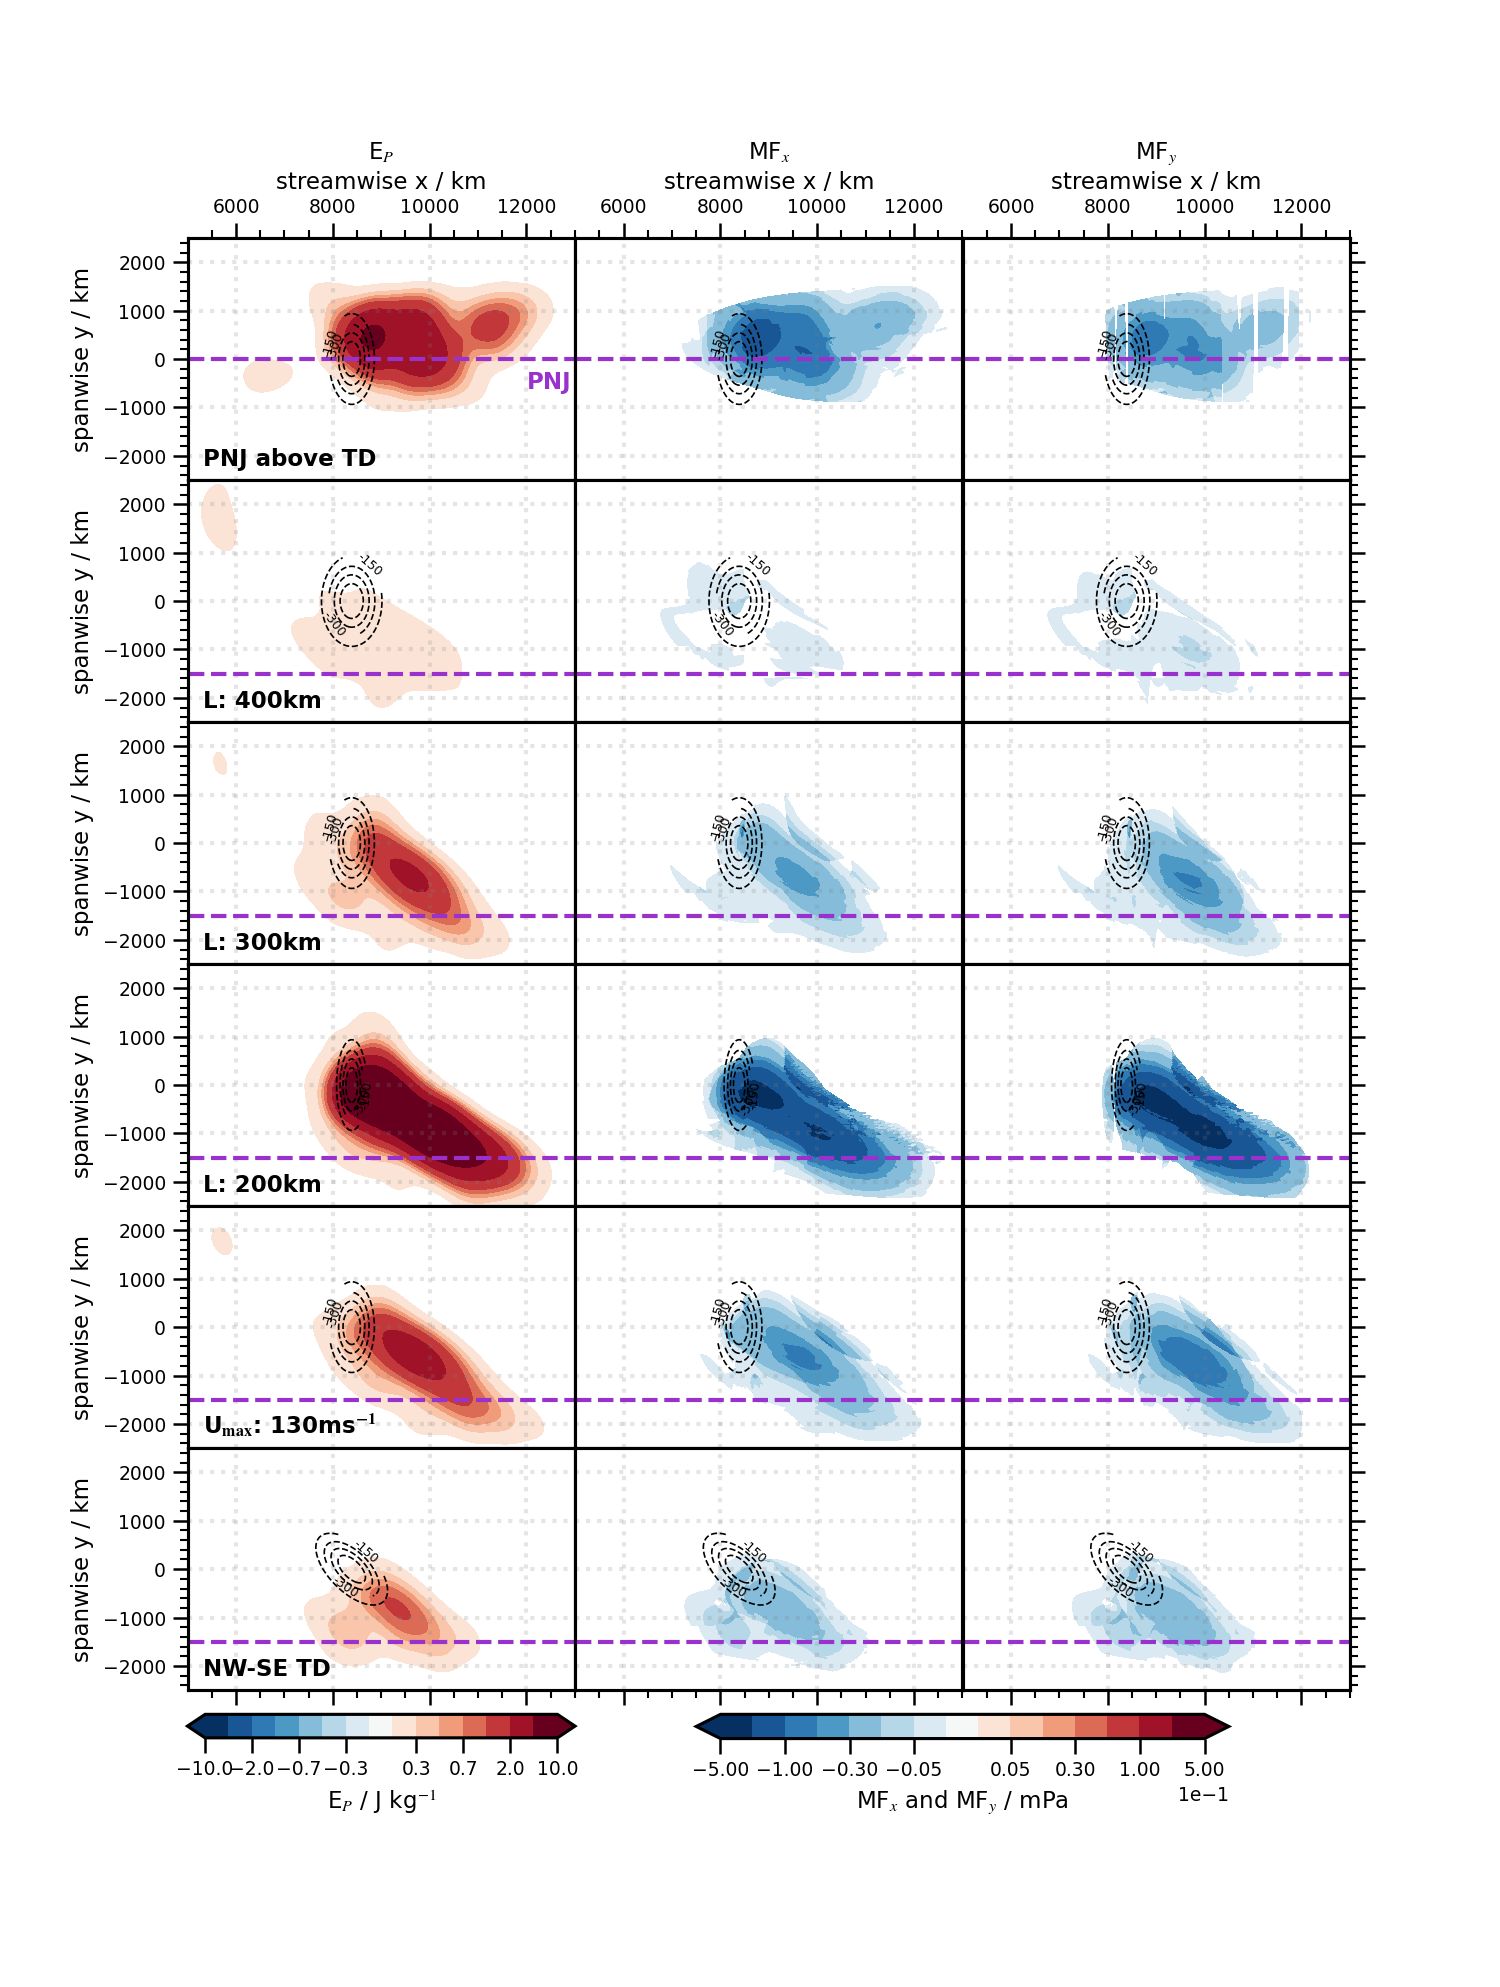
\includegraphics[width=0.99\textwidth]{figures_3D/waveletAna_fluxes_obs.png}
    \caption{Horizontal cross sections at 40km above the tropopause for five simulations with horizontal and meridional shear in a barotropic environment. Shown are $\theta$', $\lambda_x$ and $\lambda_y$ at 72h into the simulation. Dominant zonal and meridional wavelengths for each grid point are determined from wavelet analysis.}
    \label{fig:waveletAna_dudy}
\end{figure*} 
\newpage
\thispagestyle{plain}

% ==== CHAPTER 4 ===============================================================
% ---- set some counters to zero:
\setcounter{equation}{0}
\setcounter{table}{0}
\setcounter{figure}{0}
% ---- include tex-file:
\chapter{NOGWs excited by tropopause depressions in a 2D plane}
\label{sec:resultsQ3D}
% The sensitivity of 

\begin{tcolorbox}[]
    (R1) How sensitive are NOGWs from propagating tropopause folds to the 2D shape of the depression and the stratospheric environment?
\end{tcolorbox}


% define quasi 3d simulations
Following the results of the model validation / comparison of GWD with linear solutions




\section{Quasi-3D reference Simulation}
\label{sec:resultsq3D-reference}


For the stratosphere the assumption of a two atomic gas  possible to de


\begin{figure*}[tbp]
    \centering
    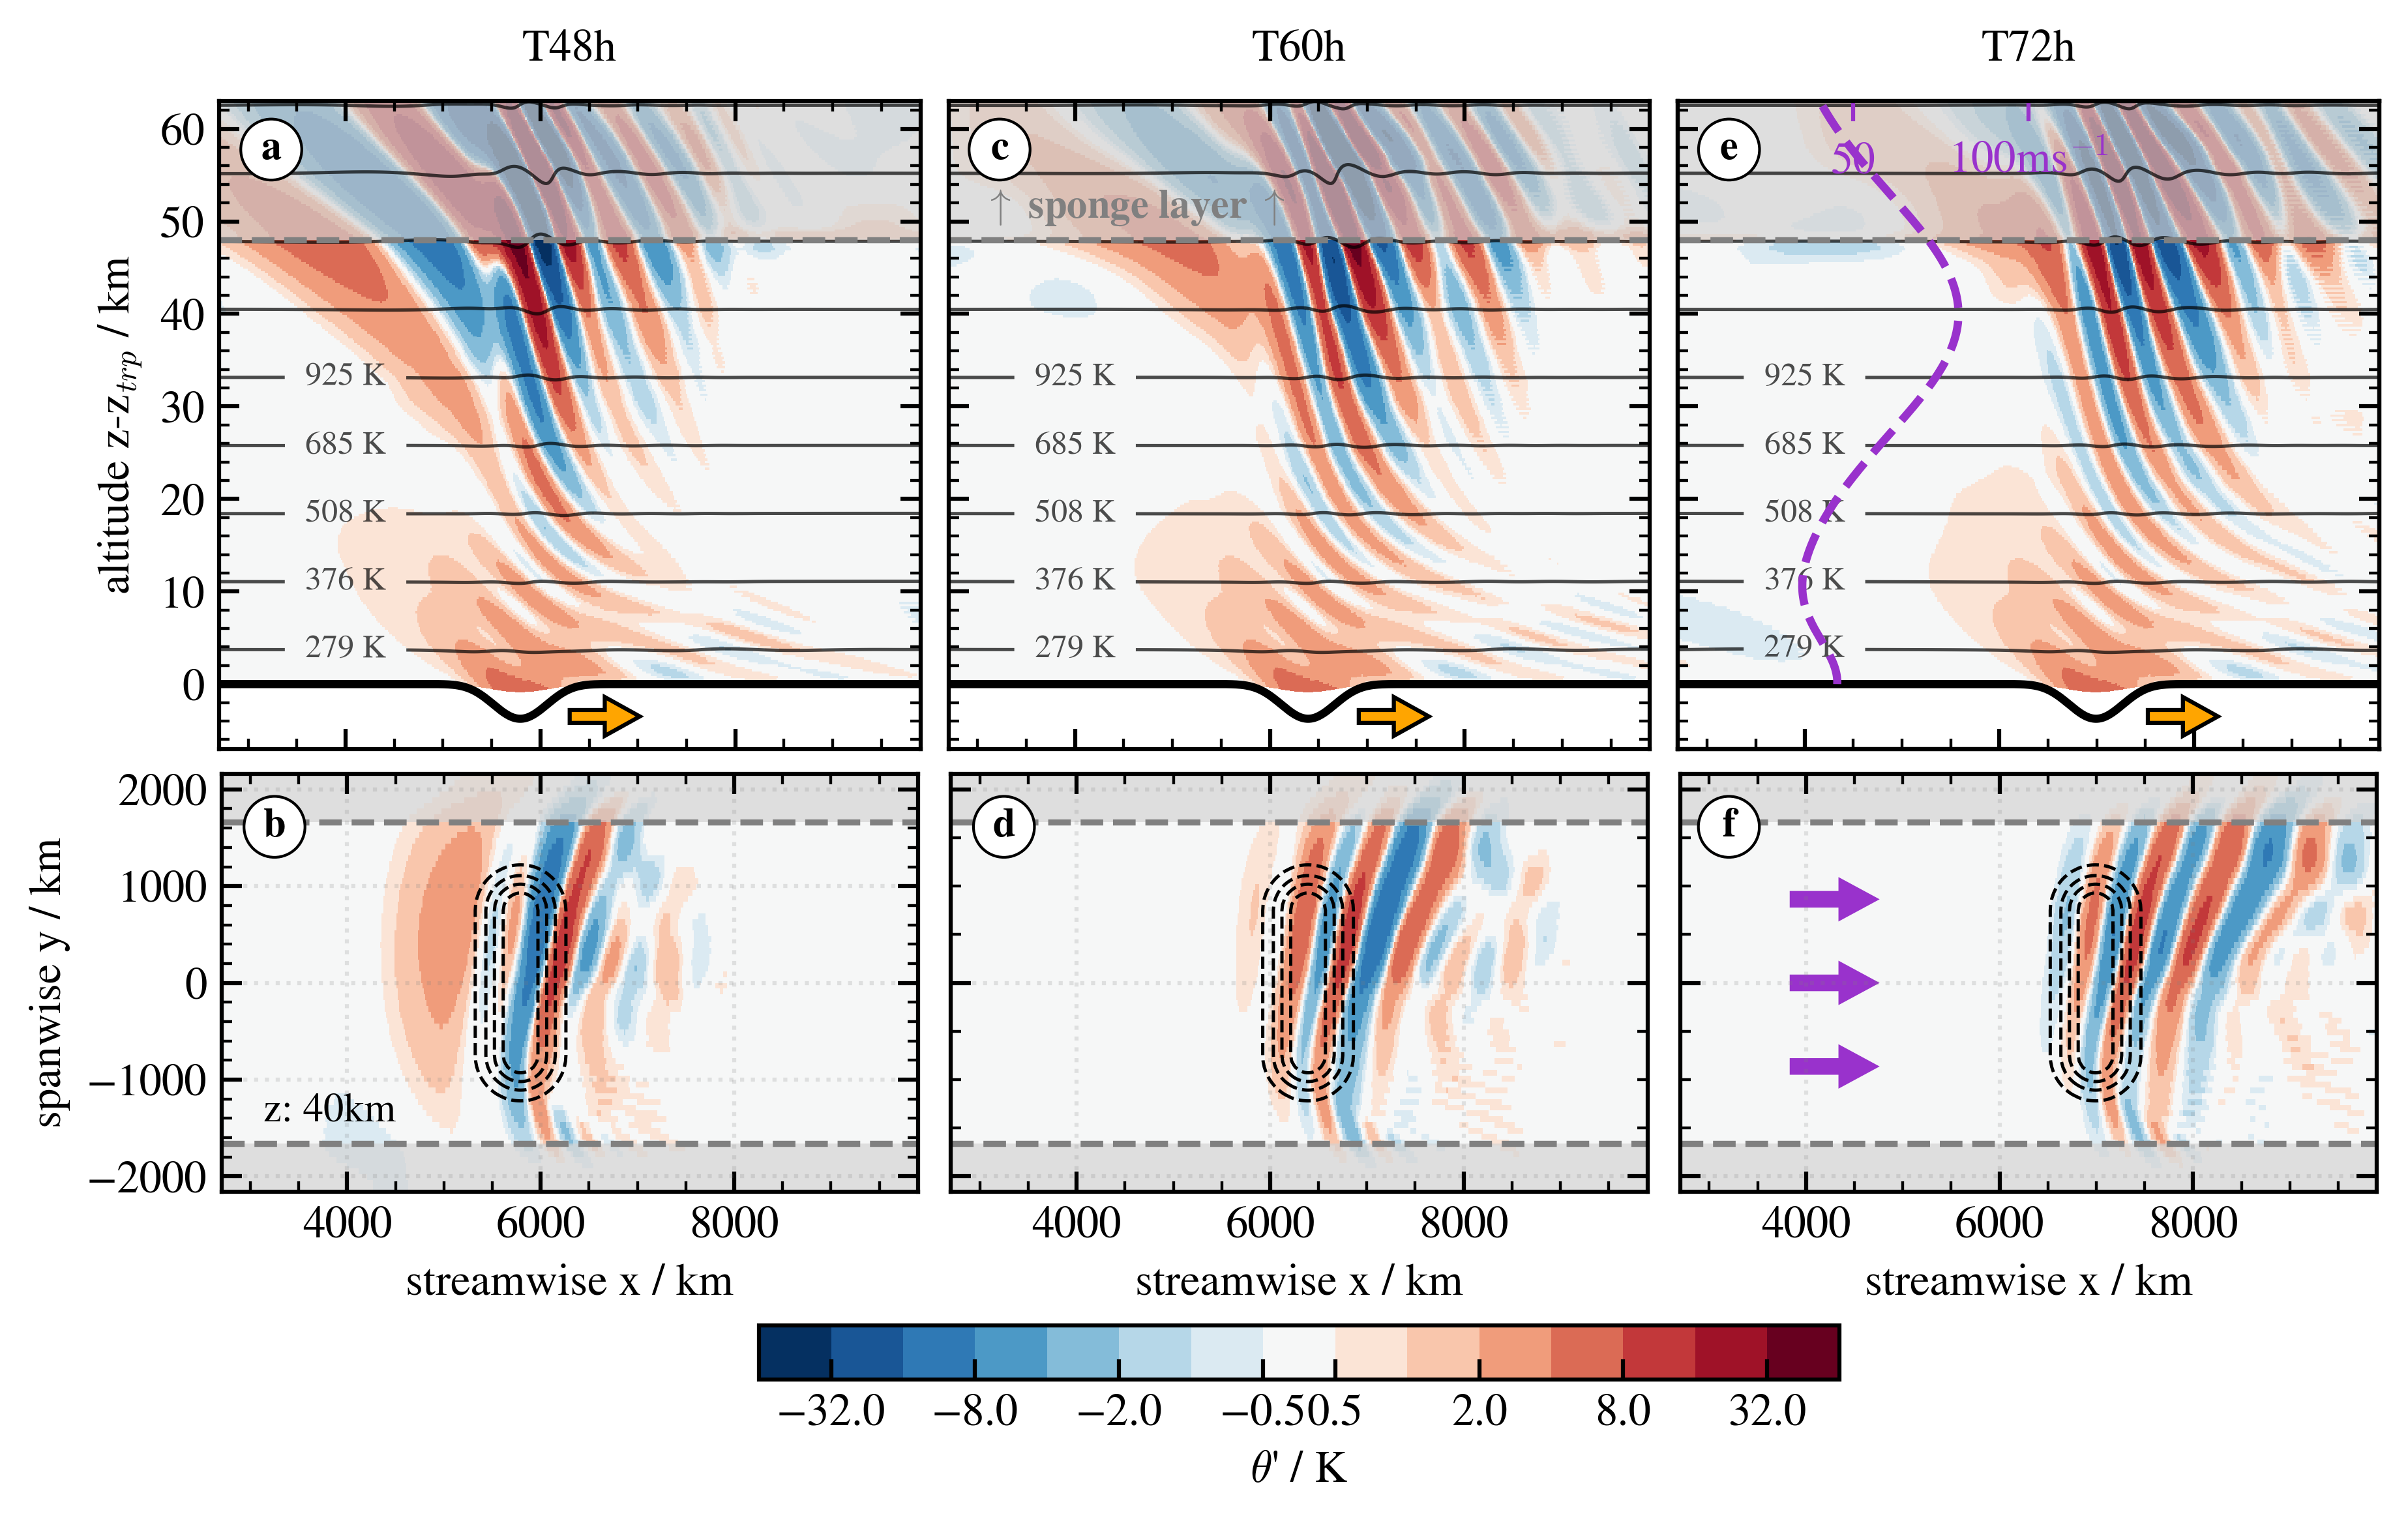
\includegraphics[width=0.99\textwidth]{figures_q3D/Q3D-th-referenceSim.png}
    \caption{Horizontal cross sections at 40km above the tropopause for five simulations with horizontal and meridional shear in a barotropic environment. Shown are $\theta$', $\lambda_x$ and $\lambda_y$ at 72h into the simulation. Dominant zonal and meridional wavelengths for each grid point are determined from wavelet analysis.}
    \label{fig:q3D_referenceSim}
\end{figure*}

\section{Influence of tropopause shape}
\begin{figure*}[tbp]
    \centering
    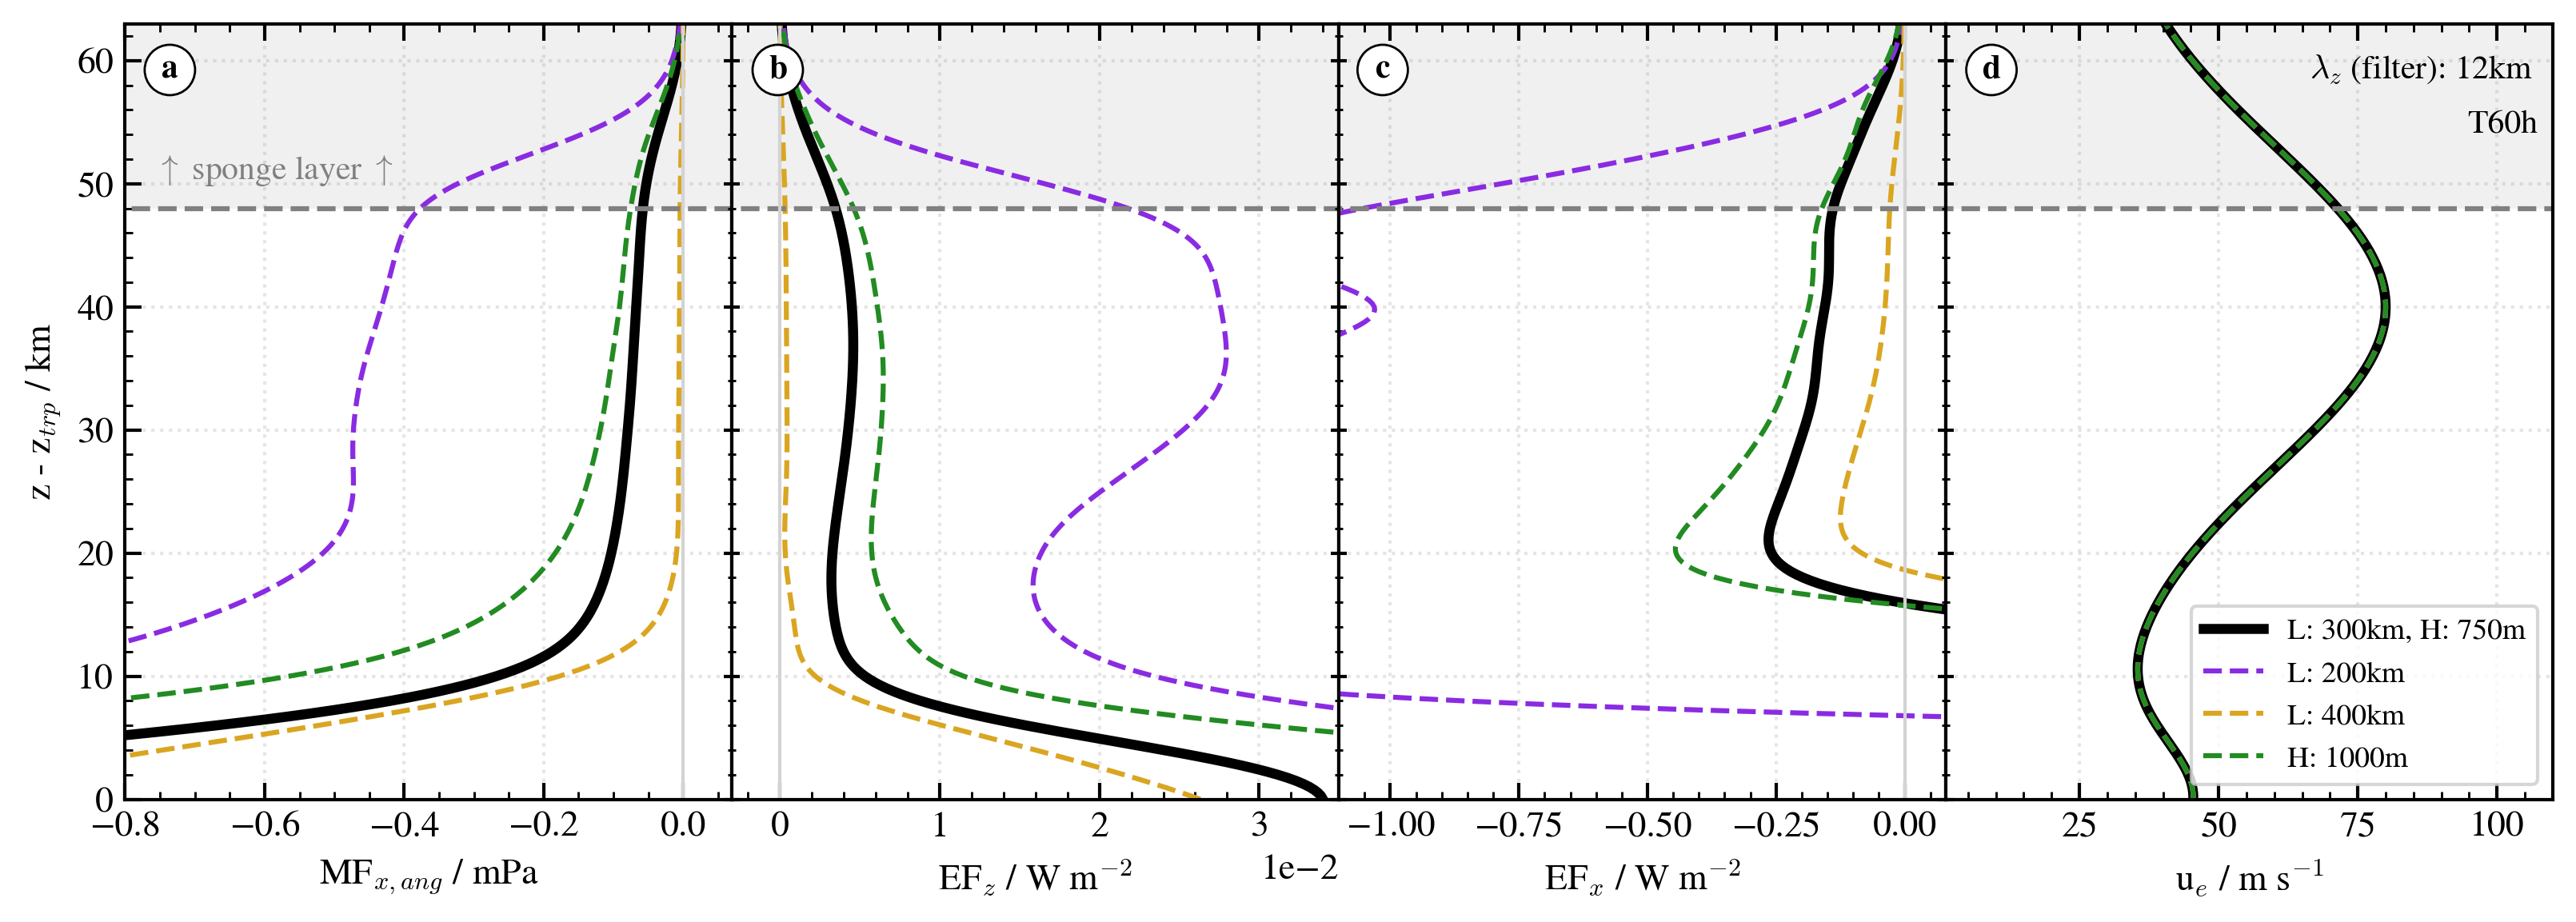
\includegraphics[width=0.99\textwidth]{figures_q3D/TD-zprofiles-translbq3D_shape-T60h-avg.png}
    \caption{Horizontal cross sections at 40km above the tropopause for five simulations with horizontal and meridional shear in a barotropic environment. Shown are $\theta$', $\lambda_x$ and $\lambda_y$ at 72h into the simulation. Dominant zonal and meridional wavelengths for each grid point are determined from wavelet analysis.}
    \label{fig:q3D_shape}
\end{figure*}


\section{Influence of background zonal wind}
\begin{figure*}[tbp]
    \centering
    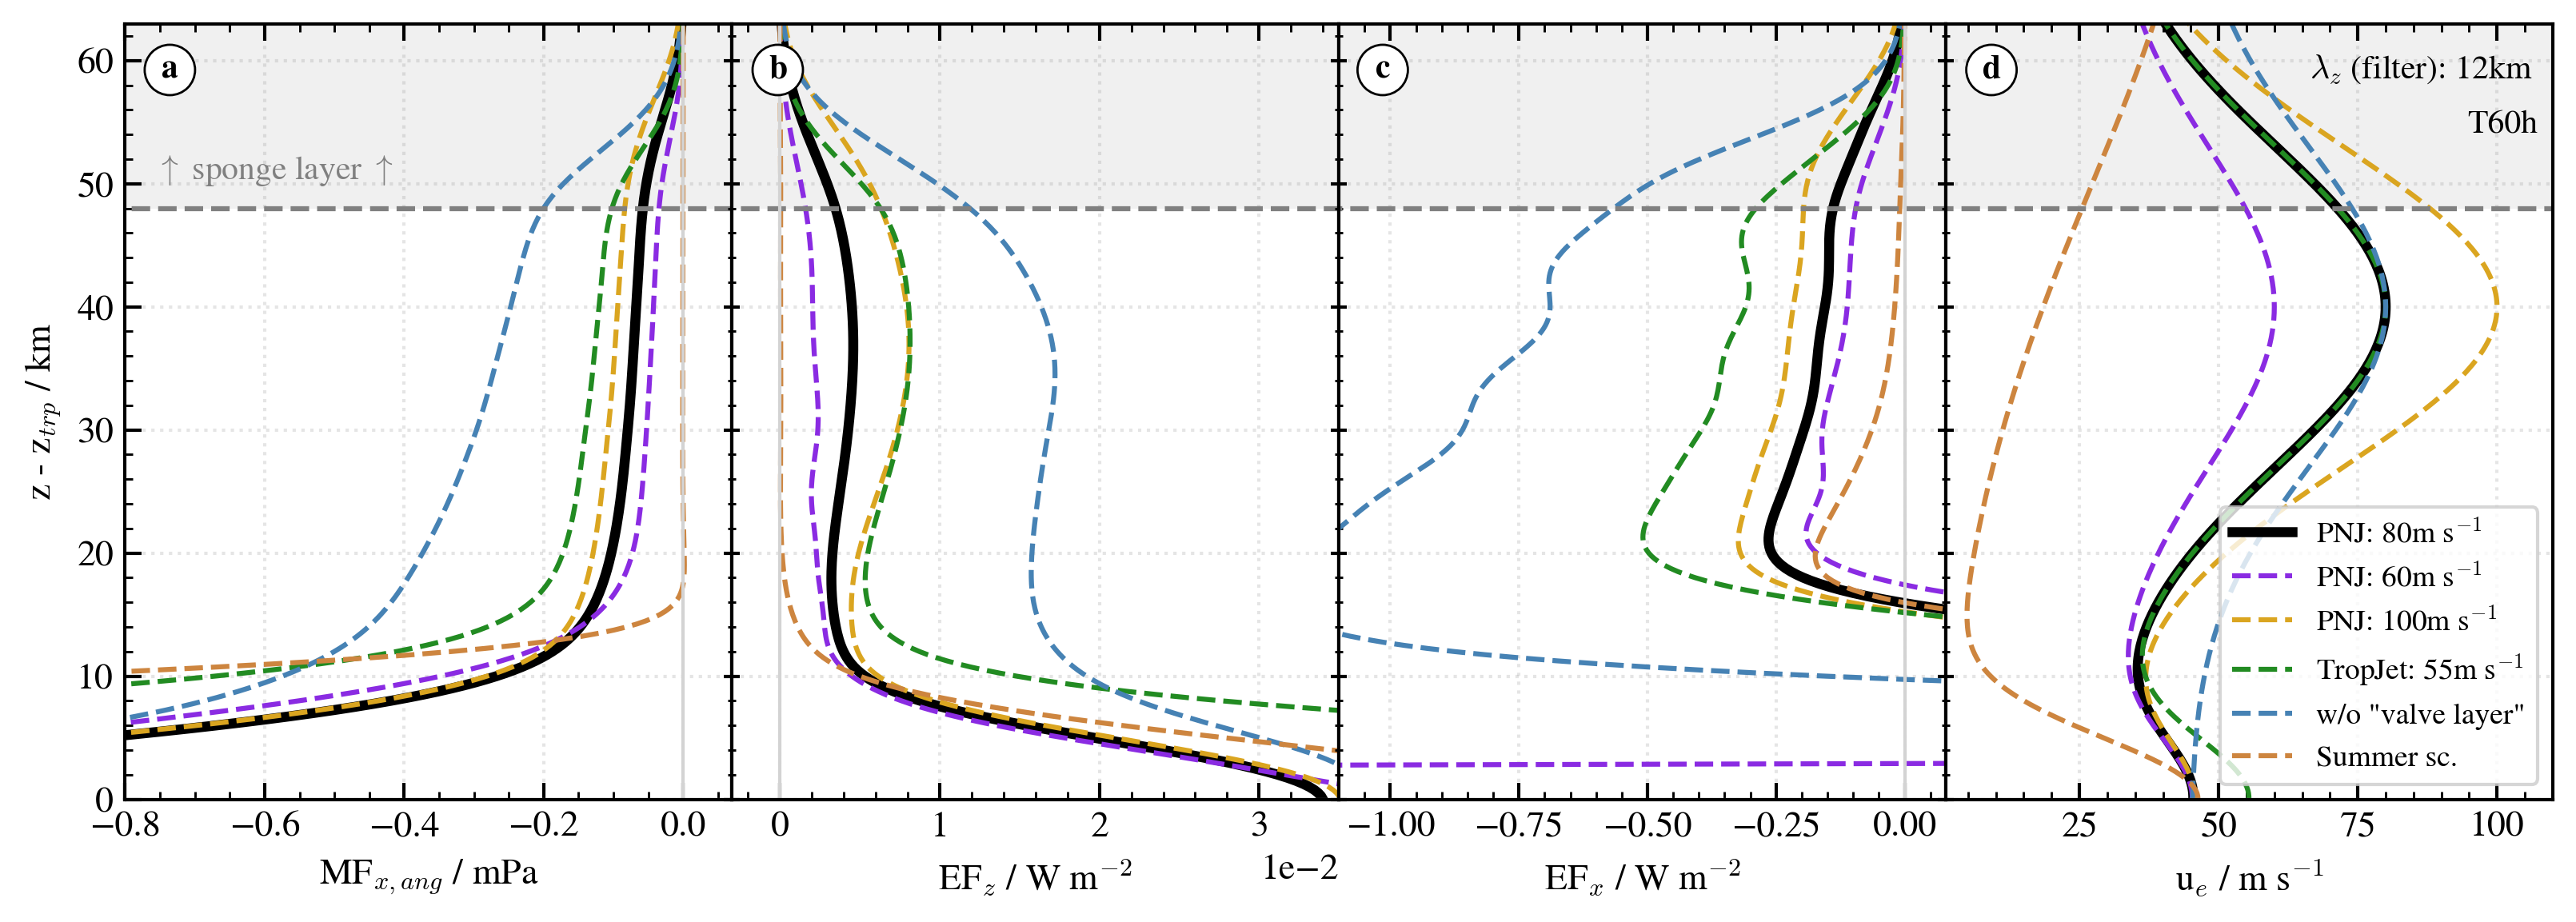
\includegraphics[width=0.99\textwidth]{figures_q3D/TD-zprofiles-translbq3D_wind-T60h-avg.png}
    \caption{Horizontal cross sections at 40km above the tropopause for five simulations with horizontal and meridional shear in a barotropic environment. Shown are $\theta$', $\lambda_x$ and $\lambda_y$ at 72h into the simulation. Dominant zonal and meridional wavelengths for each grid point are determined from wavelet analysis.}
    \label{fig:q3D_wind}
\end{figure*}

% Reflection layers in the presence of the PNJ are relevant for horizontal wavelenghts below 30-\SI{40}{\kilo\meter} (\cite[]{gill_atmosphere-ocean_1982} and Mixa), but less of a concern for the large scale inertia-gravity waves observed in our simulations.

GW starts to dissipate momentum as soon as background environment (wind profile and stability (theta profile)) approaches a critical level. In theory, the momentum is only absorbed at the critical level, but in reality GWs are not even able to reach the critical (vertical wavelength and vertical group velocity vanishes). Thus, the dissipation process should be more understood as an continuous process that starts as soon as the GW approaches a critical level due to changing background conditions. In addition, a three dimensional flow has a continuous spectrum if critical levels due to a turning of the wind with height. 


convective instability vs. shear instability 
check paper andreas norway

Figure --- and ... tell the same story. The absence of a wind minimum above the tropopause jet has the largest effect on the energy fluxes or the vertical flux of horizontal momentum. Though wind speeds at the tropopause level or the altitude of the PNJ are similar to the reference simulation, the flux towers in Figure ... and the zonal averages in figure ... show significantly higher values for the simulation without negative shear above the tropopause jet. How can this phenomenon be explained in the context of significant publications (\cite[]{eliassen_transfer_1960} or \cite[]{bretherton_momentum_1969}) that consider dissipation only in the context of a critical level. 

%Varying wind speeds with altitude could lead to critical levels. An internal gravity wave reaches a critical level when its horizontal phase speed $c_{p,x}$ is equal to the background wind. This results in a vanishing intrinsic frequency or for inertia-gravity waves in an inertial oscillation with $\hat{\omega}=f$. In the case of stationary mountain waves $c_{p,x}$ and a critical levels exists when U(z)=0. For the propagating tropopause fold $c_{p,x}=c_{tf}=\SI{13.88}{\meter\per\second}$ considering the MW like behaviour within the moving reference frame. Thus, 

Layers of reReflection layers have already been ruled out, 

% inertial critical levels, where Uk = ±f (or in general Uk + Vl = ±f). Jones found that in rotating flow it is the wave angular momentum
\textcite[]{teixeira_physics_2014} 


% However, the interest for flows with directional shear and critical layers (where the wave momentum is deposited over a continuous range of heights, as opposed to critical levels) has increased recently, since these flows are much more realistic
cite teixeira 2009

% Additionally, Eliassen-Palm's theorem states that, in the same circumstances, the momentum flux is constant with height except at critical levels (Broad 1995)

% For a directionally sheared flow and a 3D mountain, there is no single critical level, but a distribution of them with height, depending on the wavenumber of the gravity waves (i.e., a critical layer). This study aims to calculate the momentum flux in such situations of directional shear and 3D orography, addressed first by SG99

% According to Eliassen and Palm [1960] for linear, steady, small-amplitude, non-dissipative MW   !!! −𝐸𝐹 = 𝑢𝑀𝐹𝑥 + 𝑣𝑀𝐹𝑦 !!!


%Dissipation results from processes such as radiative damping [Fels, 1984; Zhu, 1994], wave–wave and wavemean flow interactions [Broutman and Grimshaw, 1988; Sutherland, 2000, 2001], and wave breaking and instability processes (see section 6).
fritts 2003

flux of angular momentum stays constant for IGWs.

\textcite[]{kruse_midlatitude_2016} obser

\textcite[]{kruse_gravity_2015} 

% Another important constraint on steady, linear moun- tain waves is the conservation of momentum flux with height with background wind shear (Eliassen and Palm 1960). According to Eq. (9), EFz will vary with height proportionately with u(z). Physically, this variation in EFz is caused by a conversion from mean-state shear energy to wave energy flux according to [from Eq. (9)]
% dEFz 52MFdu. (11) dz dz


% This mountain wave valve layer is distinct from a critical level. A critical level is defined as the level where the ambient wind speed through a wave (i.e., wind speed perpendicular to the phase fronts U?) is equal to the horizontal phase speed cp of the gravity wave. For a north–south-oriented stationary mountain wave (U? 5 U, cp 5 0), a critical level is a level of zero ambient zonal wind. Mountain waves of all amplitudes and scales will be almost completely attenuated at a zonal wind reversal (i.e., critical level) in this scenario (Booker and Bretherton 1967). A valve layer, however, is defined as a layer of reduced wind speed with no wind reversal or critical level (e.g., Fig. 9). Such a layer might allow small-amplitude mountain waves to be trans- mitted unaffected but might also cause larger-amplitude mountain waves to steepen, become nonlinear, and at- tenuate (e.g., between 23 June and 5 July in Figs. 8a,e,g). The valve-layer concept may also be applied to non- stationary gravity waves (i.e., cp 61⁄4 0) by consider- ing profiles of wind speed through the wave relative to the wave phase speed (U? 2 cp). Wave attenua- tion within this frequently present lower-stratospheric valve layer above New Zealand is quantitatively in- vestigated below.

However, MFx
above the valve layer is primarily controlled by the mini-
mum wind speed within the valve layer alone 


Mountain waves were strongly and nonlinearly attenuated in the valve layer above this jet,

This theoretical limit is never achieved in the real atmosphere because a host of instability and dissipation mechanisms become more likely as a wave approaches a critical level. \cite[]{fritts_gravity_2003}



\begin{equation}
    c_{gx} \approx \frac{N^2 \alpha}{m \sqrt{f^2+N^2 \alpha^2}} \approx \SI{-26.9}{\meter\per\second} 
    %\label{}
    % (phase propagation against the background wind results in a negative horizontal scale $k$ and, thus, negative $\alpha$)
\end{equation}
with a negative $m$ for upward propagating waves and the vertical group velocity
\begin{equation}
    c_{gz} \approx -\alpha c_{gx} \approx \SI{0.36}{\meter\per\second}
    % \label{equ_lid:cgz}
\end{equation}


\section{Influence of Coriolis force and stratification}
% make one section



\section{The influence of the fold's propagation speed}
% difference due to rising mountain?? 
\begin{figure*}[tbp]
    \centering
    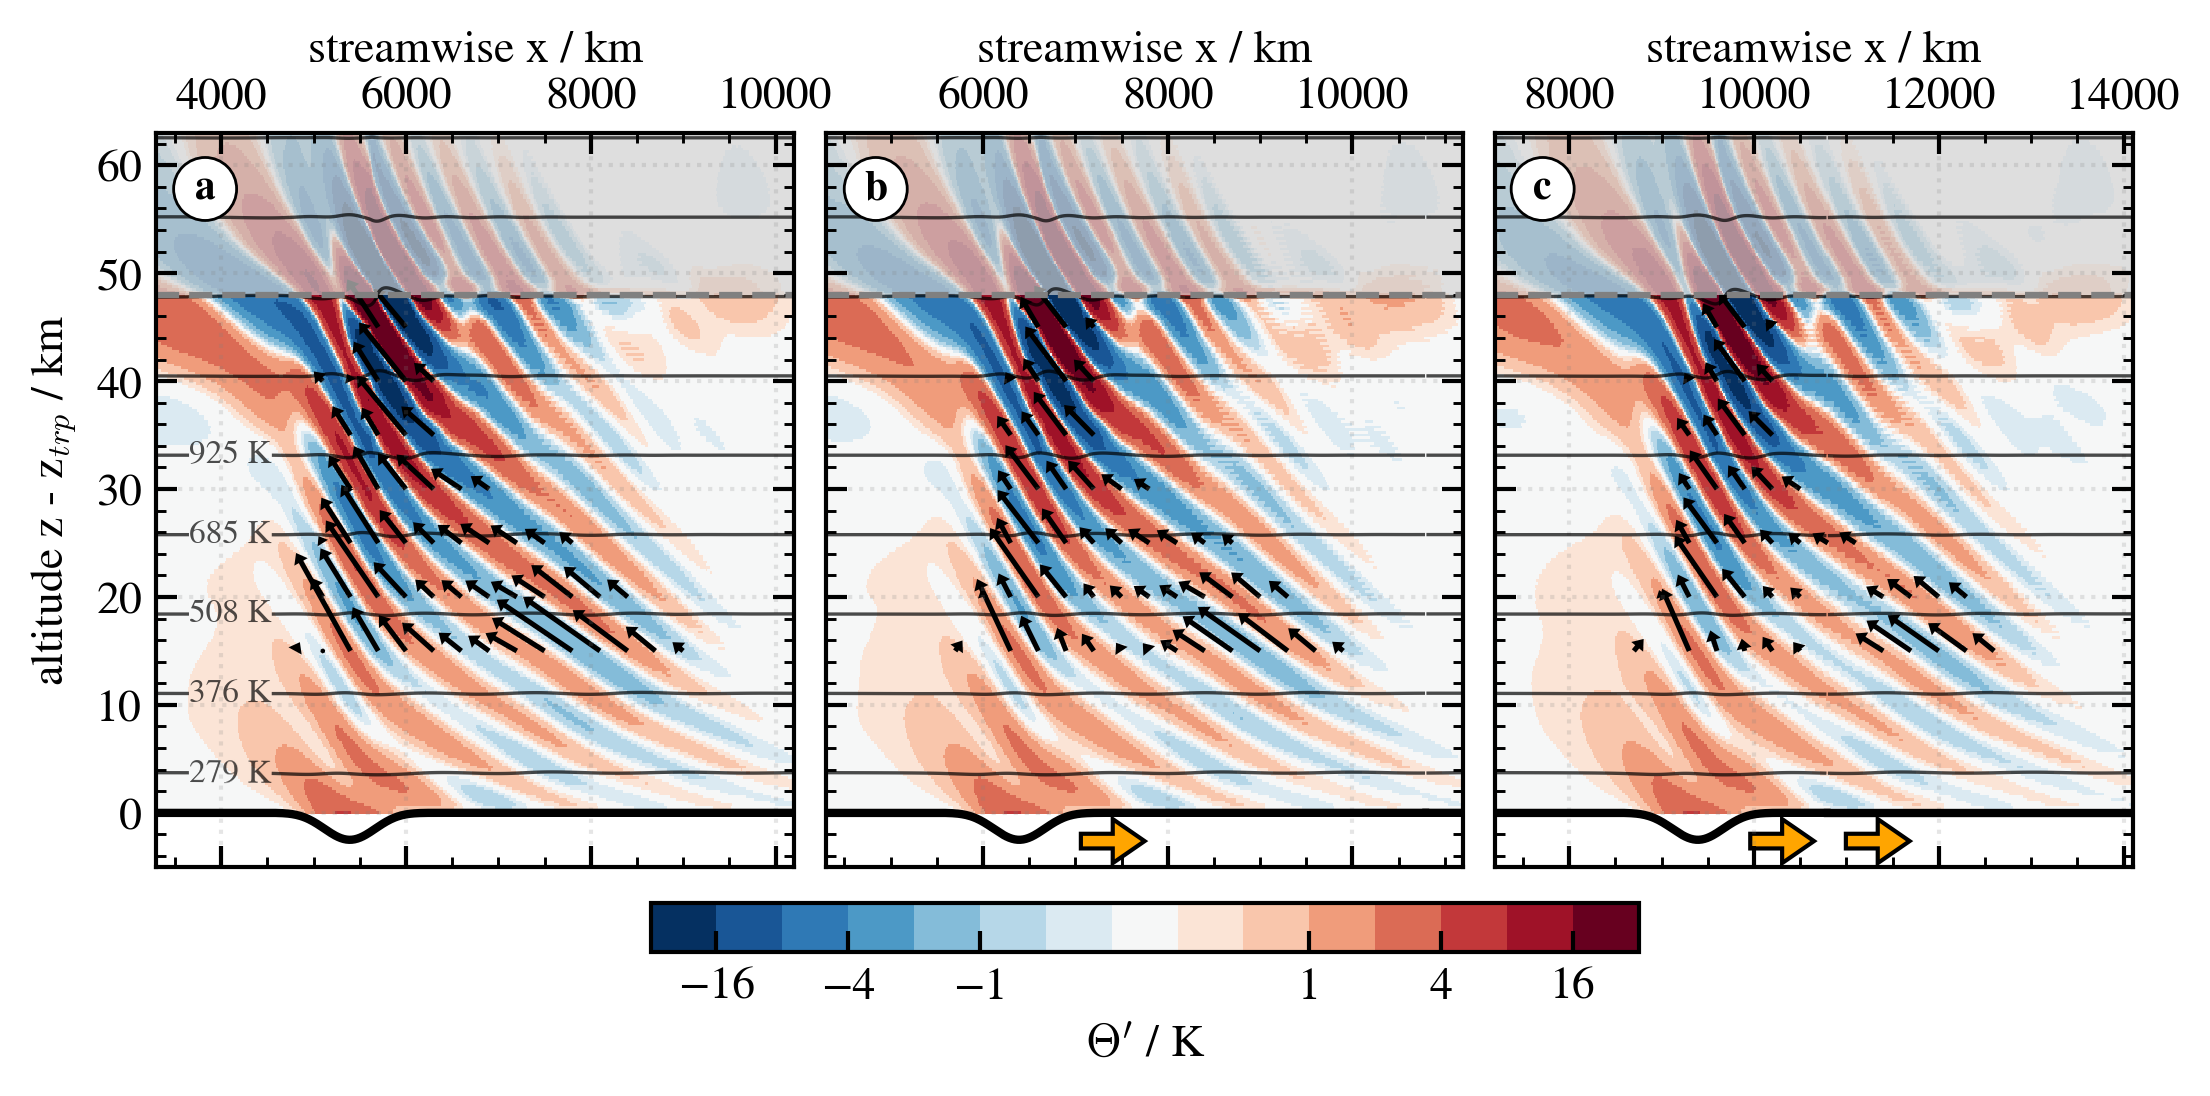
\includegraphics[width=0.99\textwidth]{figures_q3D/Q3D-TH-EF-ctropo.png}
    \caption{Shown are potential temperature perturbations $\Theta'$ overlayed by normalized vectors of \textbf{EF} for three different simulations with a constant wind profile. (a) represents the "MW case" with a stationary lower boundary. In (b) the tropopause fold moves with $c_{tf}$ and the backround wind is increased by $c_{tf}$. In (c) the tropopause fold moves with $2c_{tf}$ and the backround wind is increased by $2c_{tf}$.}
    \label{fig:q3D_ctropo}
\end{figure*}
This last section probably provides the most fundamental result of this chapter. Simulations with different propagation speeds of the tropopause fold at the lower boundary showed that the wave forcing within a reference frame moving with the fold only depends on the relative difference between the background wind speed $U$ and the fold's propagation speed $c_{tf}$. Thus, it is possible to define a 
\begin{equation}
    U_{MW}(z) = U(z)-c_{tf}
\end{equation}
that produces an identical GW forcing with a stationary tropopause fold as the propagating case. The complete vertical wind profile has to be reduced by $c_{tf}$ to achieve this phenomenon. Figure \ref{fig:q3D_ctropo} visualizes an example showing three simulations with different propagation speeds of the lower boundary, but a consistent $U_{MW}=\SI{31.12}{\meter\per\second}$. Small differences in the wave fields are most likely related to varying interactions with the sponge layer at the upper boundary, but the overall GW response within the reference frame looks almost identical. The energy flux \textbf{EF} shown in the three simulations (Figure \ref{fig:q3D_ctropo}) allows a similar conclusion. As expected, its direction is always parallel to the phase lines, but magnitudes vary slightly between the simulations. On this basis, further properties of NOGWs from propagating tropopause folds could be derived from the research on MWs.

\section{Summary and answer to research question (R1)}

\begin{tcolorbox}[]
    (R1) How sensitive are NOGWs from propagating tropopause folds to the 2D shape of the depression and the stratospheric environment?
\end{tcolorbox}
\newpage
\thispagestyle{plain}

% ==== CHAPTER 5 ==============================================================
% ---- set some counters to zero:
\setcounter{equation}{0}
\setcounter{table}{0}
\setcounter{figure}{0}
% ---- include tex-file:
\chapter{Meridional propagation of GWs excited by tropopause depressions}
\label{sec:results3D}

Eventually eight full 3D simulations were conducted to investigate the effect of a tilted TD and horizontal wind shear on the meridional propagation of GWs.
Three simulations without horizontal shear an


Add another simulation with a stronger PNJ and stronger horizontal shear to observe 
\section{Effects of TD orientation in atmosphere}
% no meridional shear


\section{Variations of the TD's zonal width and its effect on the meridional propagation of GWs}

extrinsic frequency is conserved along the ray. Is 0 for stationary mountain waves.

intrinsic frequency = 




\section{The impact of rotating the TD with respect to the zonal}
% no meridional shear

- Wavelet analysis described earlier

- 

\begin{figure*}[tbp]
    \centering
    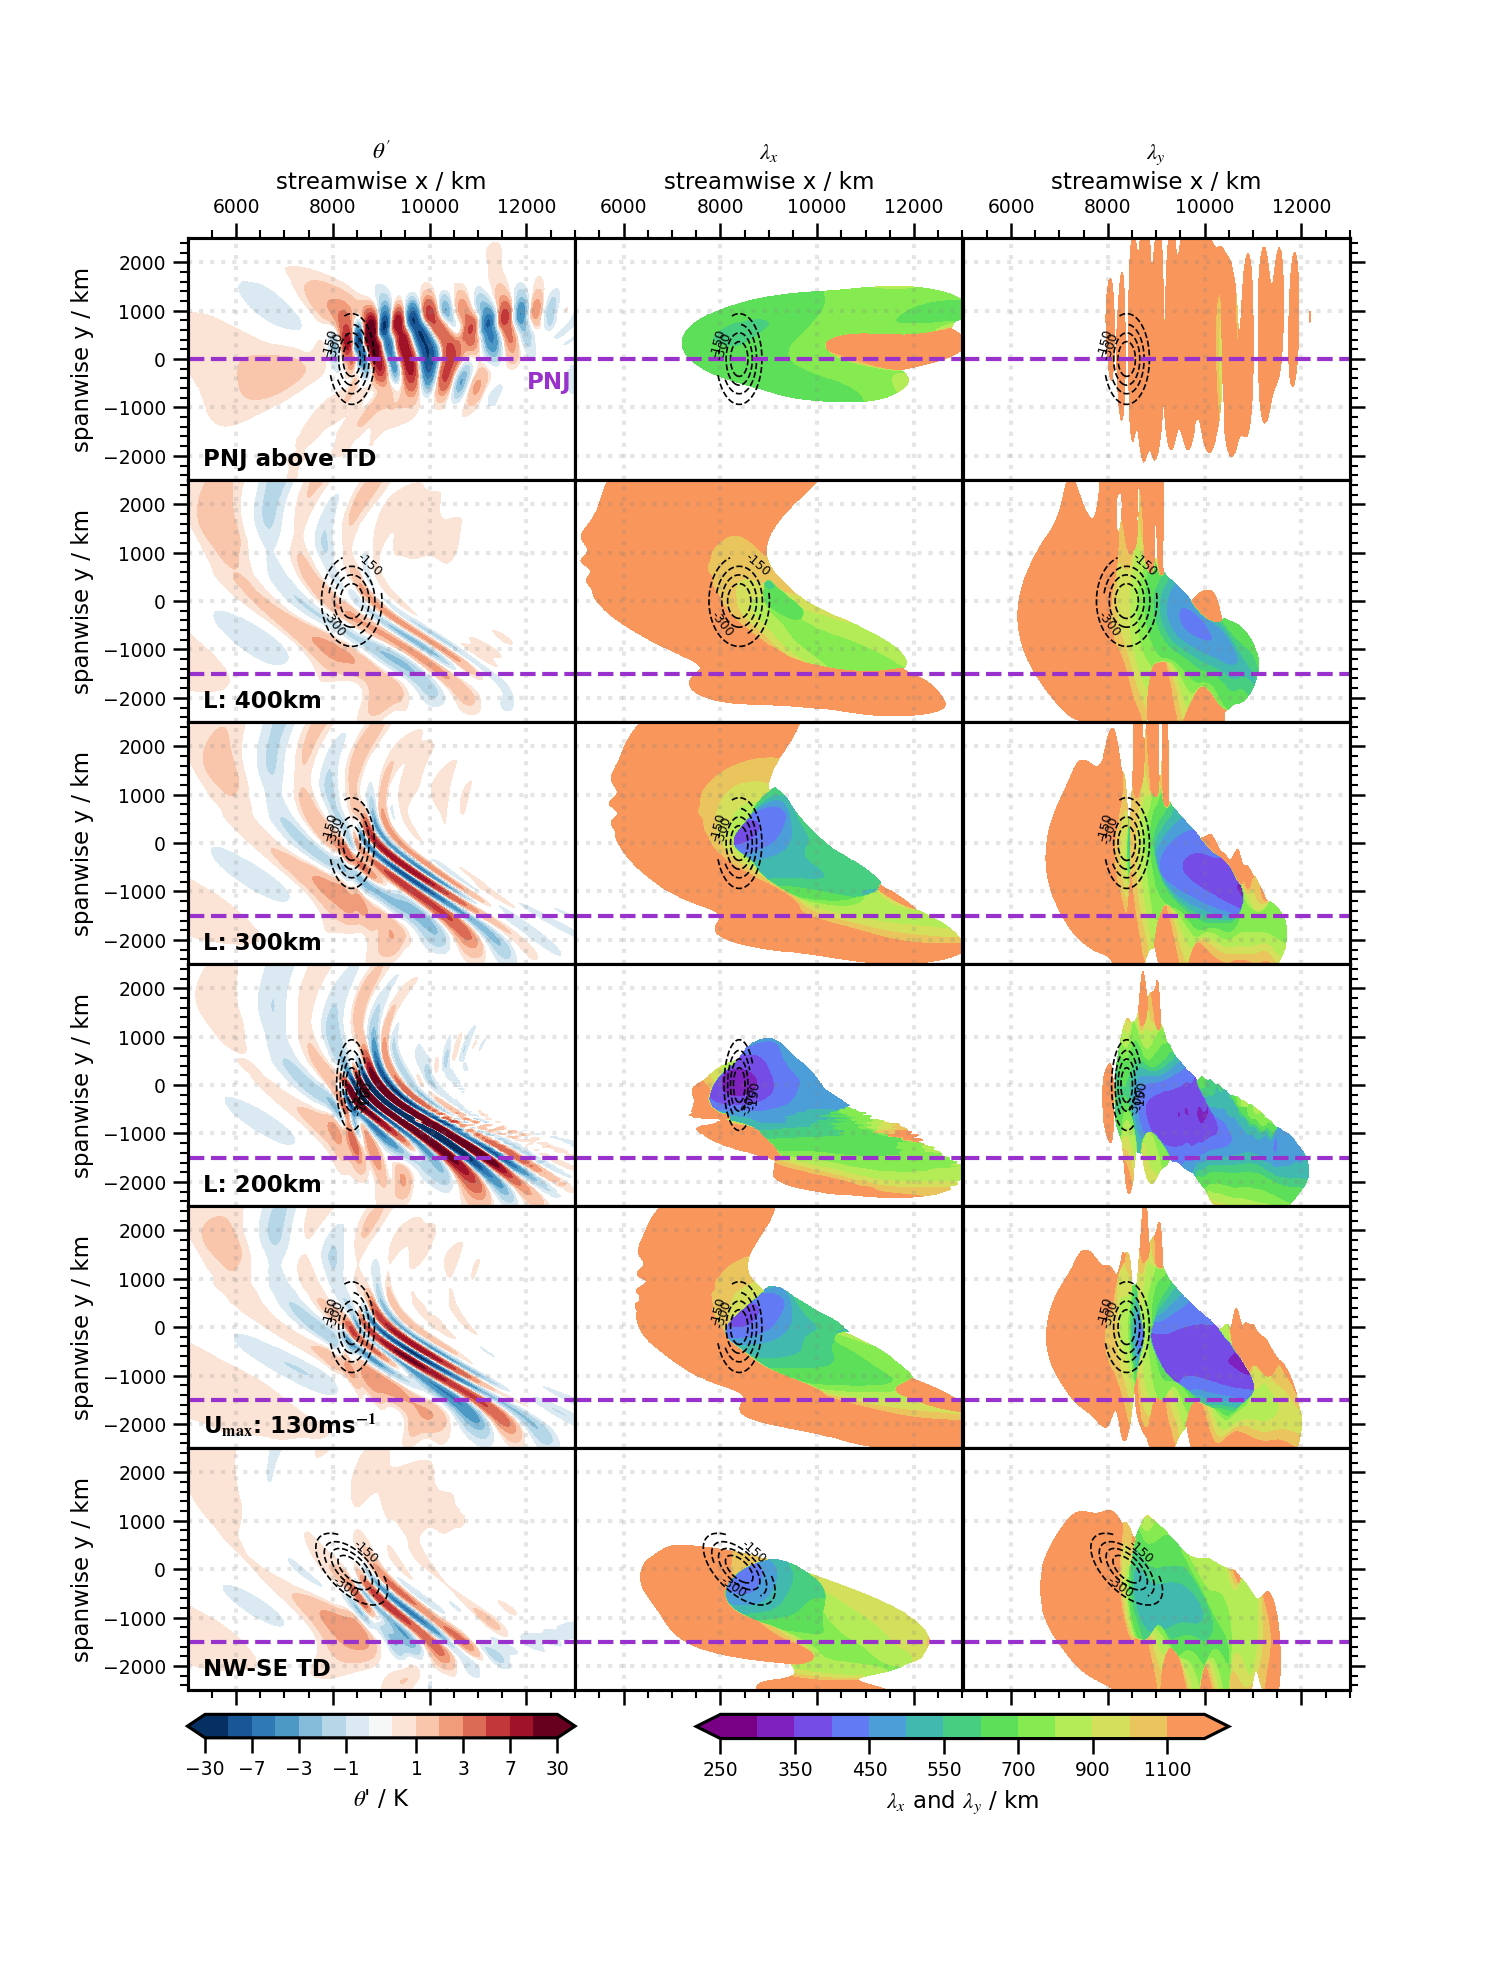
\includegraphics[width=0.99\textwidth]{figures_3D/waveletAna_dudy.png}
    \caption{Horizontal cross sections at 40km above the tropopause for five simulations with horizontal and meridional shear in a barotropic environment. Shown are $\theta$', $\lambda_x$ and $\lambda_y$ at 72h into the simulation. Dominant zonal and meridional wavelengths for each grid point are determined from wavelet analysis.}
    % \label{fig:waveletAna_dudy}
\end{figure*}


\section{Momentum fluxes from a simulation-based and observational perspective}

MF$_x$ MF$_y$ can be calculated directly from wind perturbations ($u'$, $v'$,$w'$) provided by the numerical simulation with the EULAG model. However, most satellite or ground-based observations measure temperature perturbations without further information on the corresponding wind (e.g. \cite{hindley_gravity_2019}, \cite{kaifler_compact_2021}, \cite{wu_satellite_1996}). For 2D Lidar observations these measurements usually aren't sufficient to derive horizontal momentum fluxes without additional information or assumptions for horizontal wavelengths. In the case of three dimensional datasets, as analysed by \textcite{hindley_18year_2020} (satellite observations), the determination of momentum fluxes is possible under the midfrequency approximation. This analysis follows \textcite{ern...} and combines the calculation of the potential energy (equation PE) with a three dimensional spectral analysis to obtain corresponding wavenumbers. Zonal and meridional momentum fluxes are 

\begin{equation}
    (\mathrm{MF}_x, \mathrm{MF}_y) = \frac{\rho}{2} (\frac{g}{N})^2 (\frac{T'}{\bar{T}})^2 (\frac{k}{m},\frac{l}{m})
\end{equation}

% with $\rho$ being the density, $g$ the gravitational acceleration, N the Brunt‐Väisälä frequency, $T'$ and $\bar{T}$ temperature perturbations and background temperature respectively and $k,l,m$ are zonal, meridional and vertical wavenumbers (\cite{ern}). This relation is valid for hydrostatic and nonrotational GWs with an intrinsic frequency in the range $f \ll \hat{\omega} \ll N$, where $f$ is the inertial frequency (e.g., Fritts & Alexander, 2003).

Maybe it makes sense that MFx via wavelet analysis is smaller, because it collapses contribution to a single frequency

\begin{figure*}[tbp]
    \centering
    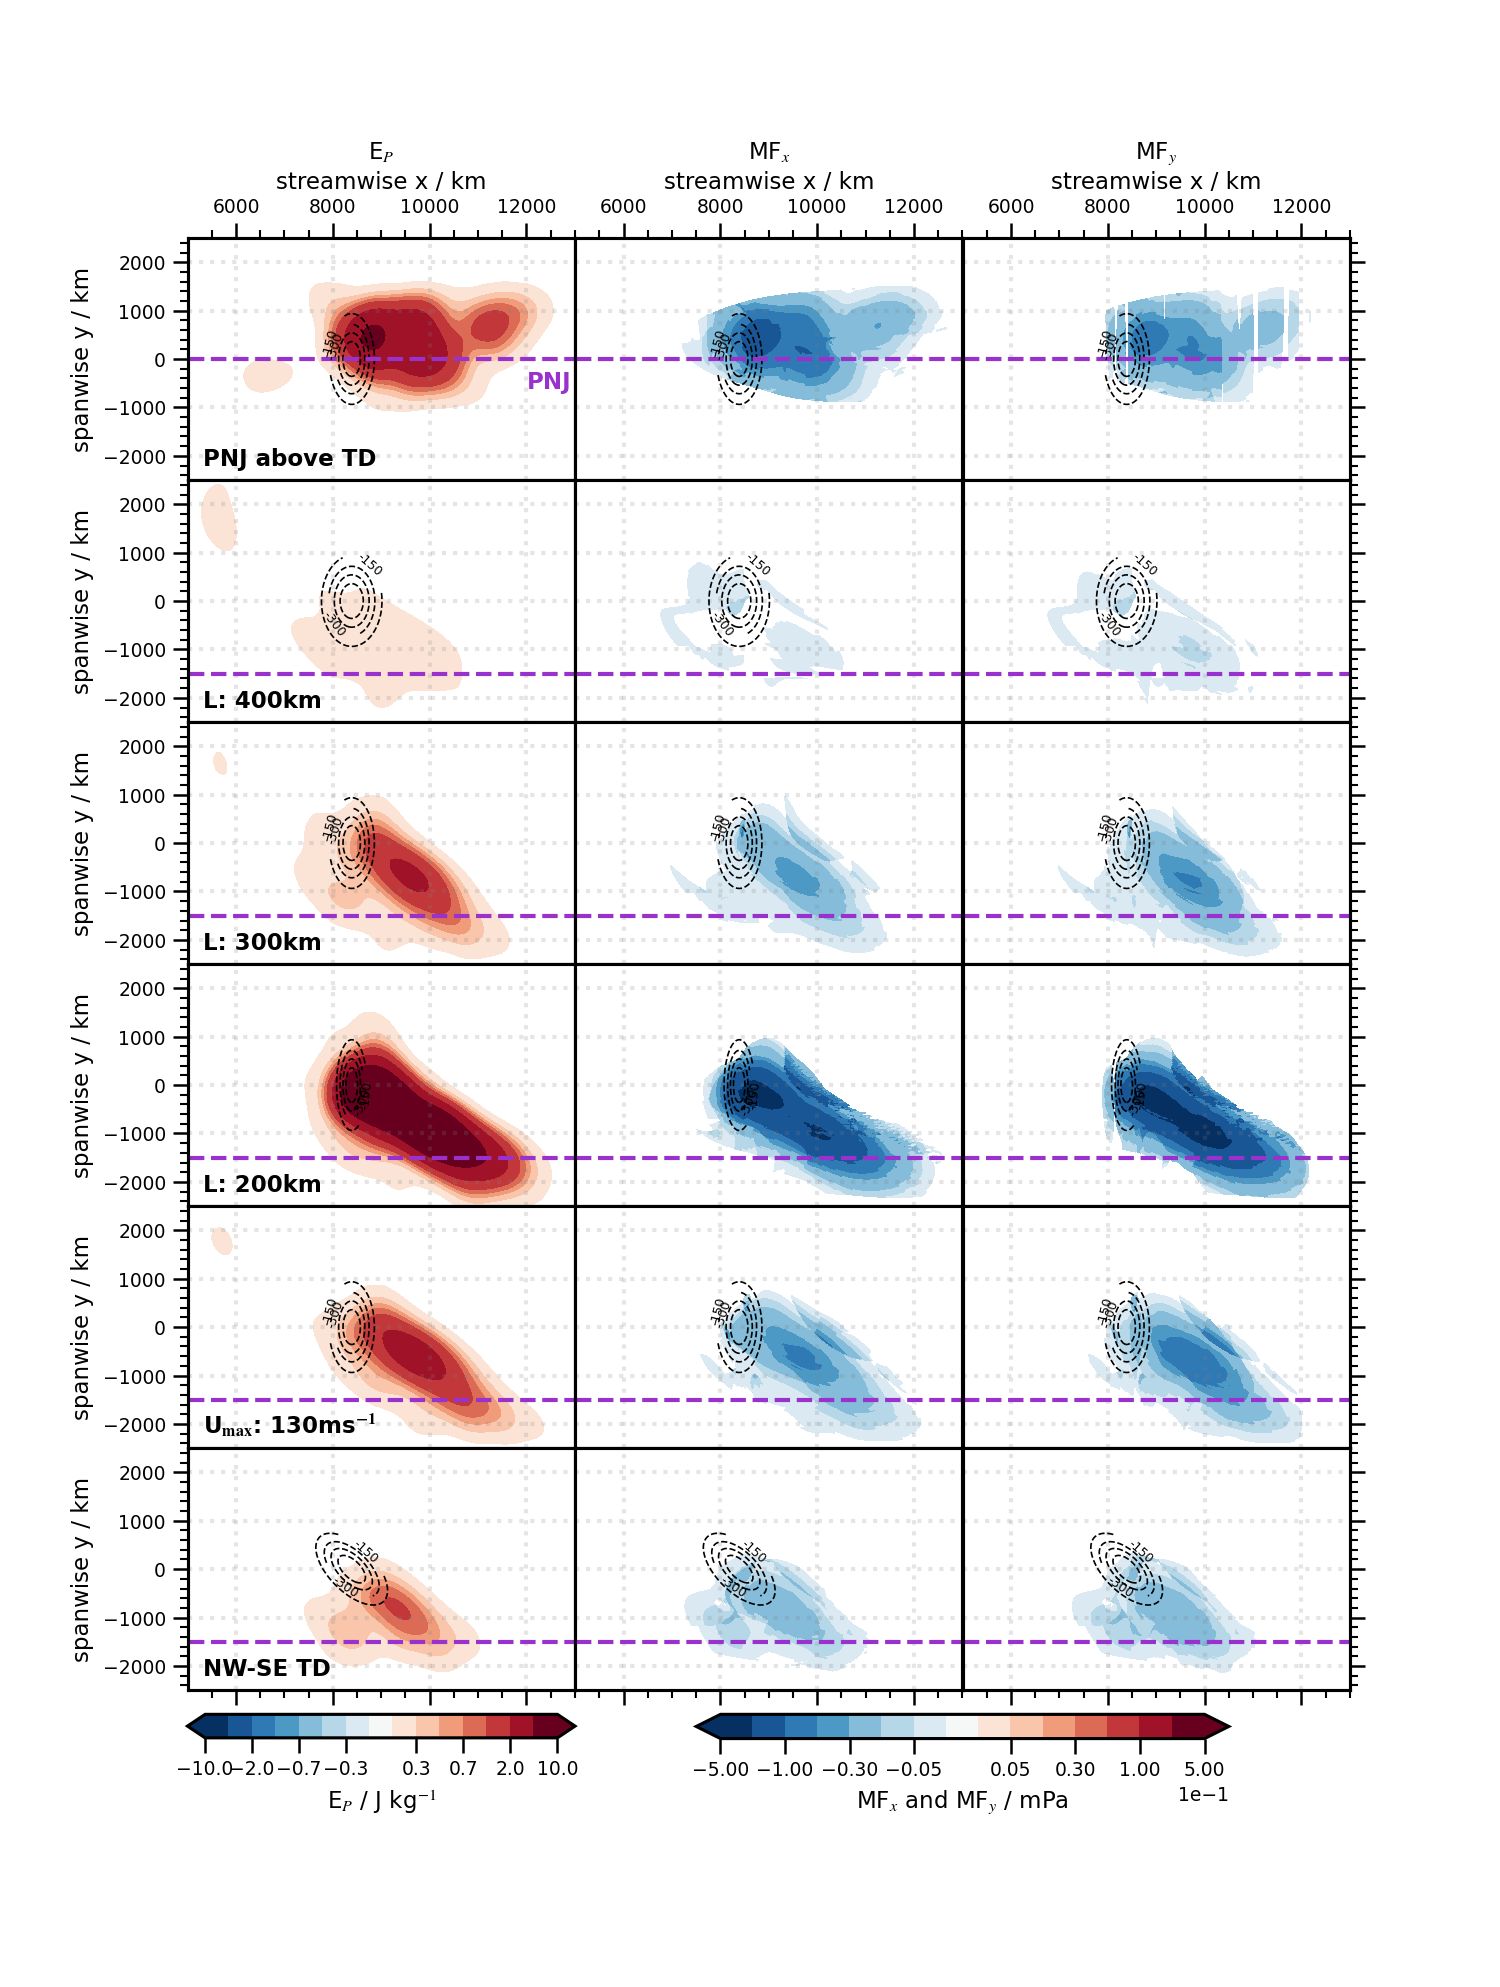
\includegraphics[width=0.99\textwidth]{figures_3D/waveletAna_fluxes_obs.png}
    \caption{Horizontal cross sections at 40km above the tropopause for five simulations with horizontal and meridional shear in a barotropic environment. Shown are $\theta$', $\lambda_x$ and $\lambda_y$ at 72h into the simulation. Dominant zonal and meridional wavelengths for each grid point are determined from wavelet analysis.}
    % \label{fig:waveletAna_dudy}
\end{figure*}

\begin{figure*}[tbp]
    \centering
    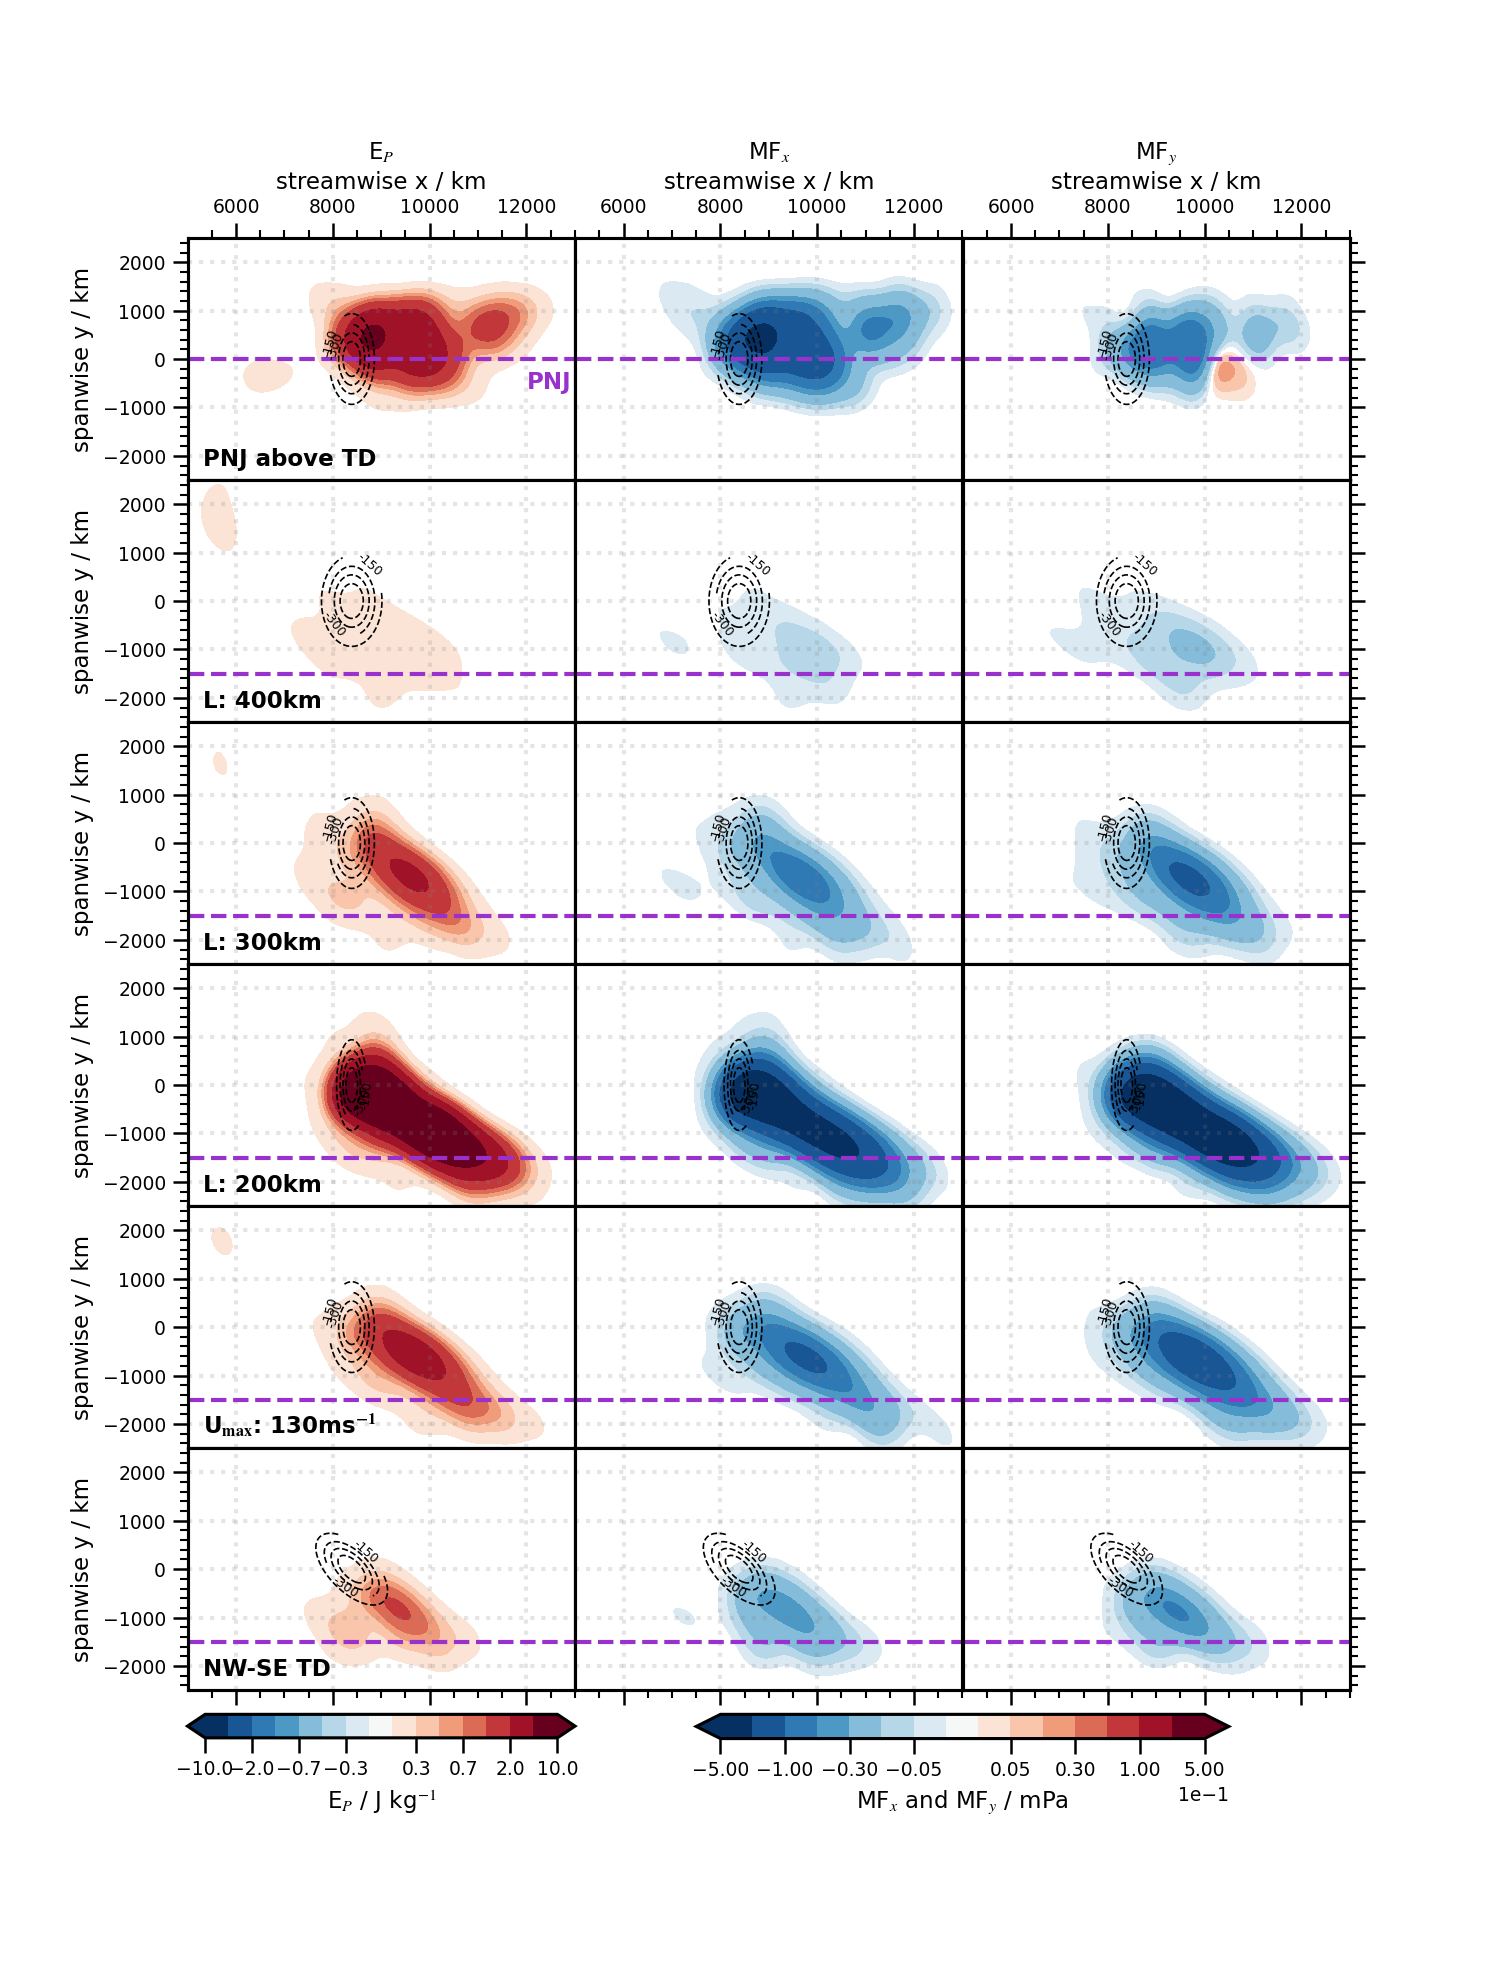
\includegraphics[width=0.99\textwidth]{figures_3D/waveletAna_fluxes_sim.png}
    \caption{Horizontal cross sections at 40km above the tropopause for five simulations with horizontal and meridional shear in a barotropic environment. Shown are $\theta$', $\lambda_x$ and $\lambda_y$ at 72h into the simulation. Dominant zonal and meridional wavelengths for each grid point are determined from wavelet analysis.}
    % \label{fig:waveletAna_dudy}
\end{figure*}
\newpage
\thispagestyle{plain}

% ==== CHAPTER 6 ==============================================================
% ---- set some counters to zero:
\setcounter{equation}{0}
\setcounter{table}{0}
\setcounter{figure}{0}
% ---- include tex-file:
\chapter{NOGWs in ground-based Lidar observations}
% NOGWs 
% Lidar observations in Q3D simulations are not useful / used y position 1 instead on npy/2!! --> use local 2D simulations for analysis of these plots (eventually conduct constant wind simulation again

% interpretation
Observations of GWs in the upper atmosphere are sparse. AIRS on board of NASA’s Aqua satellite is presently the only instrument that provides temperature measurements for a limited altitude range applicable for the detection of GWs (e.g \cite[]{hindley_gravity_2019} or \cite[]{hindley_18year_2020}). Observations are available globally, but only on a daily basis and sensitive to just a portion of the gravity wave spectrum due to the so-called "observational filter" of the instrument properties (e.g. \cite[]{preusse_space-based_2002} or \cite[]{alexander_recent_2010}). Vertical temperature profiles from ground-based Lidar stations are currently the only alternative potentially available on a regular basis. They provide much higher vertical and temporal resolution on one hand, but in the end it is just a point observation limited to night-time and clear sky conditions. The analysis of GWs in these measurements is challenging and at a certain point not possible without consulting additional information from other observations or model data. 

High resolution vertical time series at multiple locations were retrieved from the idealized numerical simulations discussed in previous chapters, too. Though the proposed excitation mechanism of these NOGWs is supposed to mimic the excitation of MWs over topography, their potential appeareance in lidar observations would be different due to the propagation of their source. Therefore, section \ref{sec:lidOb-idealized} aims for a first analysis on how waves generated by propagating tropopause depressions would show up in vertical timeseries and how they could be interpreted. Subsequently, section \ref{sec:lidOb-coral} presents two measurements of the Compact Rayleigh Autonomous Lidar (CORAL) shortly described in chapter 2 that fit to the idealized simulations. A first interpretation based on ERA5 reanalysis data is discussed, but it can be anticipated that more effort in terms of a high resolution simulation would be needed to get to an explicit conclusion. 

\section{Lidar observations in idealized numerical simulations}
\label{sec:lidOb-idealized}
% The goal of the following analysis is

Wave properties of stationary mountain waves are somewhat unfavorable from a lidar observation point of view. Their horizontal phase speed vanishes ($c_{px}=0$) together with the ground-based frequency ($\omega$=0). As a result, phase lines in vertical time series of ground-based lidar observations appear horizontal and one can only derive the vertical wavelength $\lambda_z$ from the observations, but misses information on horizontal scales (e.g. \cite[]{dornbrack_interpretation_2017} or \cite[]{reichert_highcadence_2021}). Section \ref{sec:resultsQ3D} showed that NOGWs from a propagating source might develope similar properties, but within the reference frame moving with their source. Figure \ref{fig:lidar_sim} illustrates how this alters their appearance in vertical time series. As discussed in section \ref{sec:resultsQ3D}, the wave forcing of a trough moving with $c_{source}$ (\ref{fig:lidar_sim}b) for a certain point in time can be reproduced by a stationary trough with a wind profile reduced by $c_{source}$ (Figure \ref{fig:lidar_sim}c). However, phase lines in the vertical time series differ significantly and show an upward (downward) tilt for a source moving in the same (opposite) direction as the background wind (Figure \ref{fig:lidar_sim}d). Does this allow for a derivation of horizontal wave properties? Yes and no! Clearly, tilted phase lines enable the quantification of a ground-based period $T$ from the vertical time series, but linking this period to wave properties depends on the wave source and atmospheric background conditions. Multiple phenomena could explain upward tilted phase lines in lidar observations, so their intepretation requires additional knowledge on the prevailing processes and synoptic situation. Examples are:
%  so by considering lidar observations only, upward tilted phase lines could for example be attributed
% \cite[]{ern_absolute_2004}

\begin{itemize}
    \item downward propagating wave packets caused by reflection or wave breaking in the upper atmosphere which excites secondary waves that travel up and down from their source region (\cite[]{dornbrack_interpretation_2017} and \cite[]{vadas_mechanism_2003}).
    % fishbone pattern

    \item transient background conditions. Mainly in the form of a varying wind speed and wind direction.

    \item a GW source moving in the same direction as the background wind as illustreated in Figure \ref{fig:lidar_sim}d and \ref{fig:lidar_sim}f.
\end{itemize}

\begin{figure*}[tbp]
    \centering
    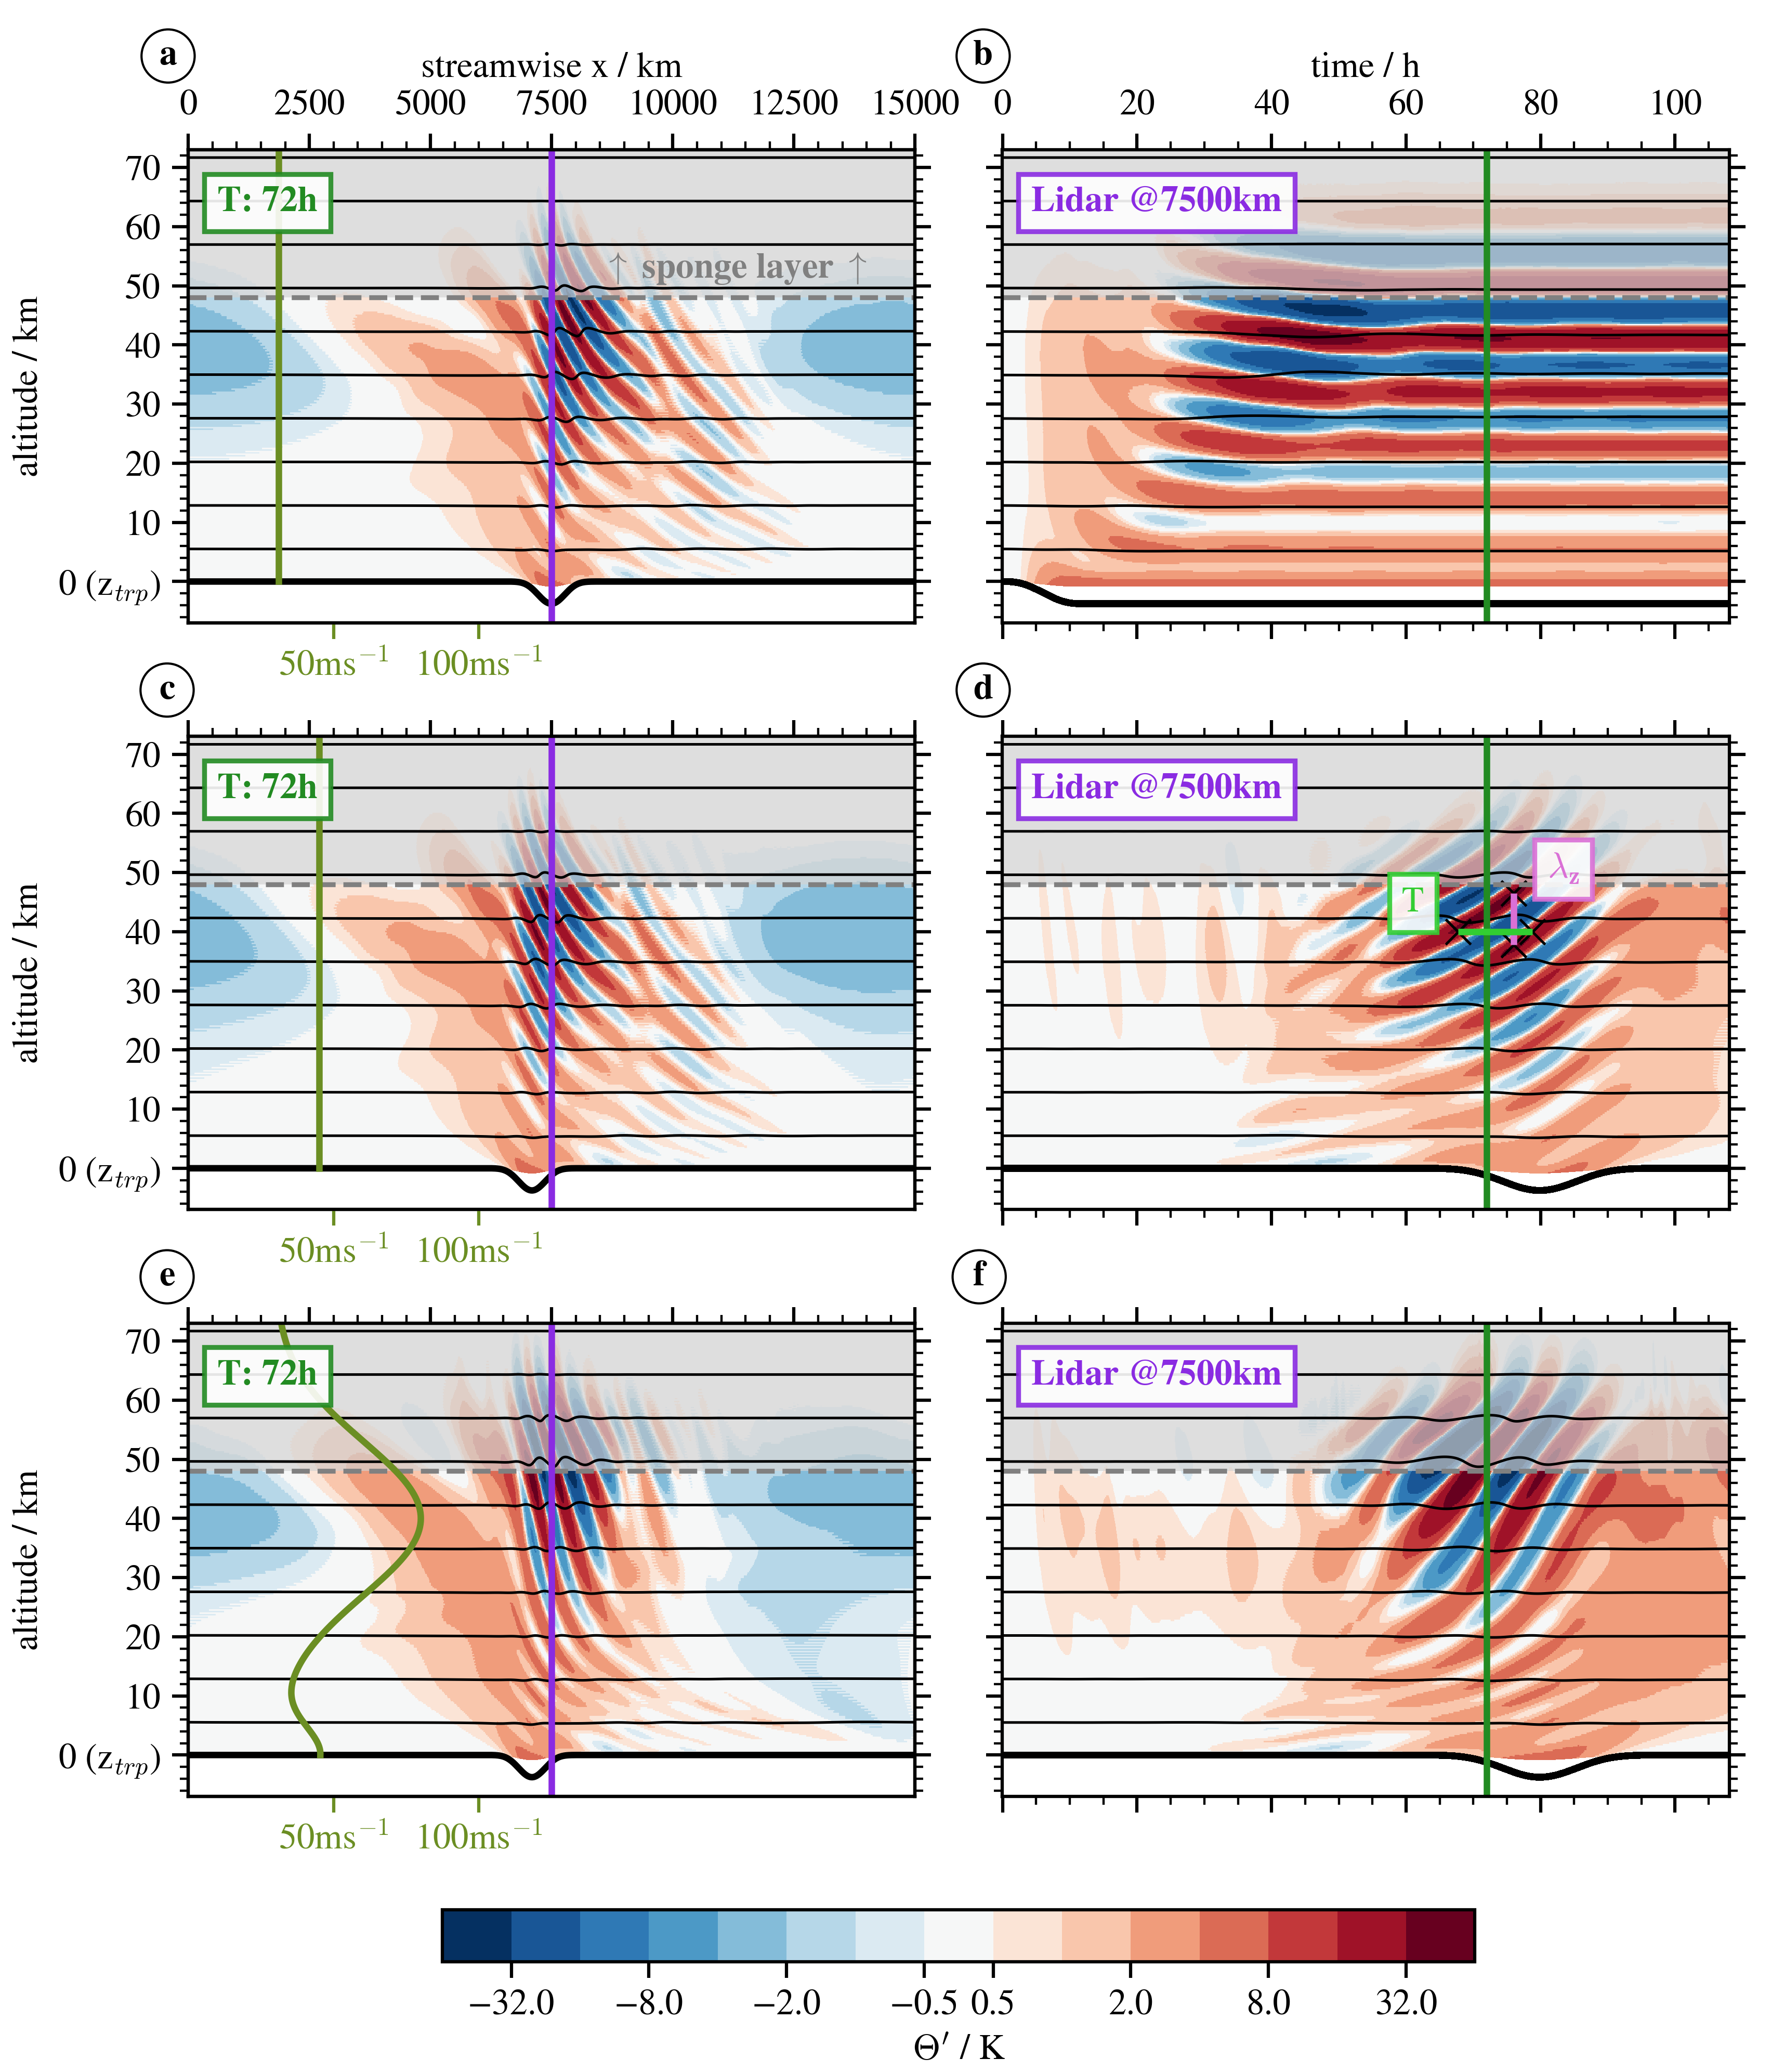
\includegraphics[width=0.99\textwidth]{figures_lidar/lidana_th.png}
    \caption{Shown are vertical cross-sections (a,c,e) after $t$=\SI{72}{\hour} with vertical wind profiles in green and vertical time series (b,d,f) at the outlined position for three different simulations. The first simulation (a,b) features a stationary obstacle at the lower boundary and a constant wind profile. In the second simulation (c,d) the trough moves to the right with a constant speed $c_{source}$=\SI{13.88}{\meter \per \second} and the wind is increased by the same amount. The last simulation (e,f) represents the reference simulation of the sensitivity analysis in section \ref{sec:resultsQ3D} with a more realistic stratospheric winter time wind profile. The assessment of $\lambda_z$ and period $T$ from the vertical time series is labeled in (d), two consecutive $\lambda_x$ are labeled in (c). Contour lines represent constant potential temperature and the amplitude of the lower boundary is scaled by a factor of 5.}
    \label{fig:lidar_sim}
\end{figure*}

Within the framework of this work, let us stay with the last explanation and think through the GW characterization for the simplified case of a constant wind profile shown in Figure \ref{fig:lidar_sim}c and \ref{fig:lidar_sim}d. To recap, a constant stratification with $N=\SI{0.02}{\per \second}$ was used for all simulations starting at the tropopause simplifying the dispersion relation for Boussinesq flows to

\begin{equation}
    \hat{w}^2 = \frac{N^2k^2}{k^2+m^2} = Ncos(\phi).
    \label{equ_lid:dispersion}
    % observed waves obey a dispersion relation for internal Boussinesq
    % Alhough variations in density are the very essence of buoyancy, they are neglected everywhere in the Boussinesq equations “except in so far as they modify the action of gravity” (Rayleigh, 1916), i.e., the density is assumed to be constant except in the buoyancy force
    % by applying a peak finding algorith to the vertical profile and additionally a time span $T$ applying the same algorithm along the time axis
\end{equation}

As labeled in Figure \ref{fig:lidar_sim}d, the vertical distance between troughs or ridges in the vertical time series yields the vertical wavelength $\lambda_z=\SI{9.25}{\kilo \meter}$ and wavenumber $m$, the horizontal distance at \SI{40}{\kilo \meter} provides a period $T=\SI{13.92}{\hour}$ and ground-based frequency $\omega$. How can this frequency be interpreted? If we assume a fully developed stationary wave field above the depression that propagates with its source, the tilt of the phase lines within the lidar observation depends on the propagation speed of the GW source and the horizontal wavelength $\lambda_x$. Thus, a constant propagation speed $c_{source}$=\SI{13.88}{\meter \per \second} leads to $\lambda_x = T \cdot c_{source}$= \SI{695}{\kilo \meter}, which is in the range of wavelengths labeled in the vertical cross-section(Figure\ref{fig:lidar_sim}c) at the same height with $\lambda_x$=\SI{525}{\kilo \meter} - \SI{712}{\kilo \meter}. The ratio of $\lambda_x$ and $\lambda_z$ provides 

\begin{equation}
    \phi = \tan^{-1}(\frac{\lambda_x}{\lambda_z}) 
    \label{equ_lid:phi}
\end{equation}

and 

\begin{equation}
    c_{px} = \frac{N}{k} cos(\phi), \qquad c_{pz} = \frac{N}{m} cos(\phi)
    \label{equ_lid:cp}
\end{equation}


vertical waIn a next step,

Continueing the analysis with this satisfying result....

angle phi

pahse speeds
group speeds

check slides






- For stationary mountain waves the . For a transient/propagating GW source this results in $c_{px}=-u+c_{source}$ with $c_{px}$ balancing the wind speed forcing described in section \ref{sec:resultsQ3D}.



Extend conclusions of \textcite{dornbrack_interpretation_2017}.

% The slope of the phase lines in a horizontal time series taken at fixed altitude is equal to cPx. from Dörnbrack -> not true for propagating source

% Summarizing the assumptions involved so far if we would like to retrieve wave properties from the virtual time series observations as presented in Figure 6:

% \begin{equation}
%     \lambda_z = \frac{2*\Pi}{m} 
% \end{equation}



% Assuming \textcite{dornbrack_interpretation_2017}., the recorded period $T = 2π/ω$ can be used to obtain an estimate of the ground-based frequency ω. In such a case, the slope of the phase lines gives the vertical phase speed cPz = ± λz/T and the propagation directions of the wave phases and of the wave packet, respectively. Using an estimate of the background stratification N, the phase angle φ can be estimated from Equation (8) and k can be computed. Technically, the Equations (12) and (13) can now be employed to derive the components of the group velocity cgx and cgz from the known values of k, m, and φ. Summarizing the assumpti

show for constant wind and idealized stratospheric winter profile

In the thorough descripition of 


As usual, the vertical wavelength in the  be derived from the Lidar observation with


\begin{equation}
\begin{aligned}
    c_{px} = \frac{N}{k} cos(\phi), \qquad c_{pz} = \frac{N}{m} cos(\phi)
    % \label{equ:momEqu}
\end{aligned}
\end{equation}



% First of all, there have to be sufficiently large tropospheric winds perpendicular to the mountain ridge for excitation of MWs (e.g., Bramberger et al., 2017; Dörnbrack et al., 1999; Kaifler, Kaifler, et  al.,  2015). In addition, Dörnbrack et  al.  (1999) report that good excitation conditions prevail when the wind turns no more than 30° within the first 30 km. Monthly mean wind speeds in ERA5 data are at about 𝐴𝐴 15 ms−1 at surface level (500 m) at all times. The wind rotation within the first 30 km is <30° during the months from March to October with a surface level forcing between 240° and 280°. Thus, in the climatological mean MWs are excited and able to propagate deep into the middle atmosphere in the winter months. A strong wind rotation within the first 30 km of about 60° can only be observed in July 2020. At this time, we also find reduced GW energies at all altitude regions (see Figure 6). For upward propagation, the wind speed in the direction of wave propagation must not become zero as this would lead to wave breaking (Lindzen,  1981). Moreover, for deep vertical propagation, the MWs should not encounter turning levels where the intrinsic frequency approaches the buoyancy frequency (e.g., Schoeberl, 1985). These conditions occur in the core of the PNJ and filter horizontally short MWs or lead to evanescent modes tunneling through the PNJ (e.g., Mixa et al., 2021). Another obstacle for MWs is the stratospheric wind minimum where the waves' 𝐴𝐴𝐴𝐴′-amplitude may become equal to the horizontal wind speed causing wave breaking. This wind minimum can act as a valve for vertically propagating MWs (Kruse et al., 2016). Figure 10 reveals that low wind speeds at ∼25 km altitude occur from March to May. In the winter months, with positive temperature gradients (Figure 2) and large horizontal wind speeds (Figure 10) up to 50 km, generally good vertical propagation conditions can be expected. Above, shear instabilities and unstable lapse rates lead to wave dissipation. On the other hand, the mesosphere is the favorable region for the generation of secondary gravity waves (Heale et al., 2020; Kogure et al., 2020; Vadas & Becker, 2019; Vadas et al., 2018). Large contributions of apparently up- and downward propagating waves and reduced contributions of stationary waves (see Table 3) at mesospheric altitudes might indicate their existence above Río Grande.



\section{CORAL observations of NOGWs from a transient source}
\label{sec:lidOb-coral}

% In addition, the latitudinal position of the PNJ over the Southern Andes can change significantly over the course of several weeks. As the PNJ is responsible for the refraction of waves toward larger vertical wavelengths, this mechanism in combination with a fixed 𝐴𝐴𝐴𝐴cut might also affect the derivation of potential energies.

This section provides a short introduction to an interesting Lidar observation of the Compact Autonomous Rayleigh Lidar (CORAL) at the southern tip of South America in Rio Grande, Argentina. 

Short description of CORAL...

Discussion of plots:

- GWs in upper atmosphere + background wind!!

- lower plot: Forcing conditions at surface 

- eventually wind profile over time could be helpful with interpretation

- state that vertical time series would look quite similar to observations - angle of idealized simulation for realistic wind profile -> approximately 20km / 12h 


- second case: time of observation could fit to tropopause fold... waves develope into the lee of the fold... but wind direction turns towards NW might be another explanation.

\textcite{kaifler_compact_2021} provide a more extensive summary on CORAL's setup and observation, 

focus on observation from July 28th, 2018 showing upwards tilted lines of constant phase between 

\begin{figure*}[tbp]
    \centering
    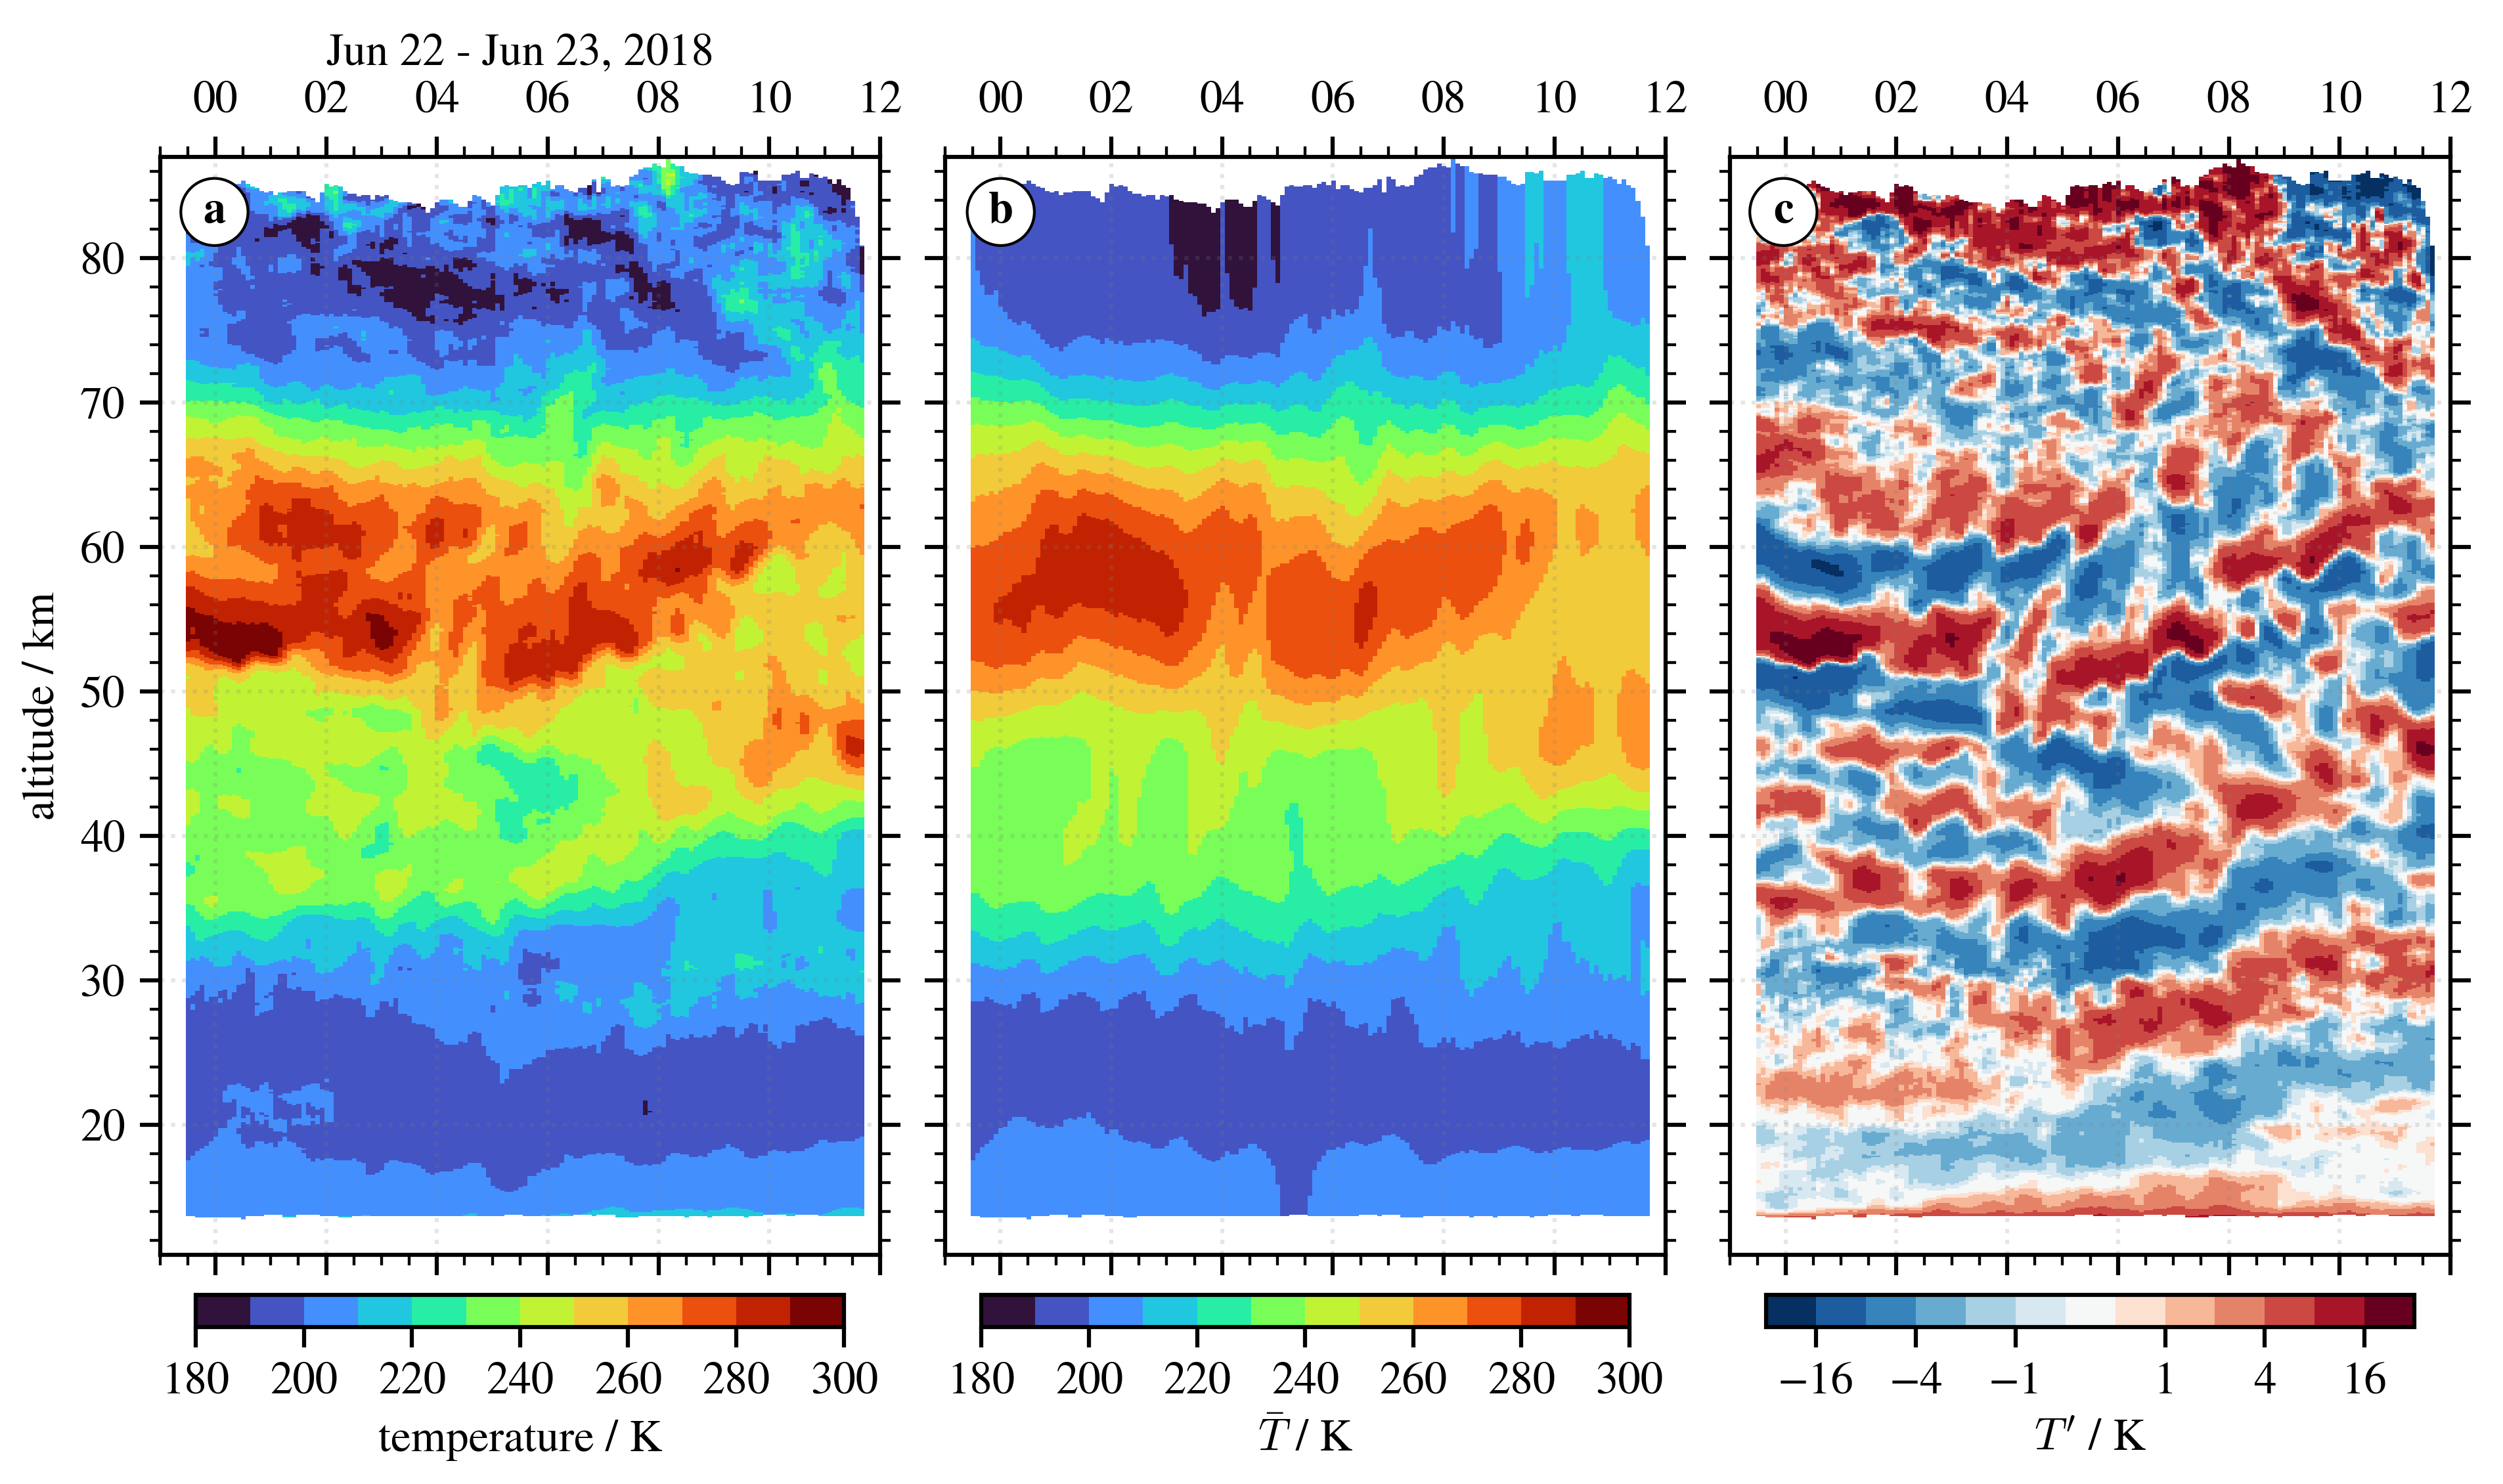
\includegraphics[width=0.99\textwidth]{figures_lidar/coral_event_20180622.png}
    \caption{Vertical cross sections at 40km above the tropopause for five simulations with horizontal and meridional shear in a barotropic environment. Shown are $\theta$', $\lambda_x$ and $\lambda_y$ at 72h into the simulation. Dominant zonal and meridional wavelengths for each grid point are determined from wavelet analysis.}
    % \label{fig:waveletAna_dudy}
\end{figure*}


\begin{figure*}[tbp]
    \centering
    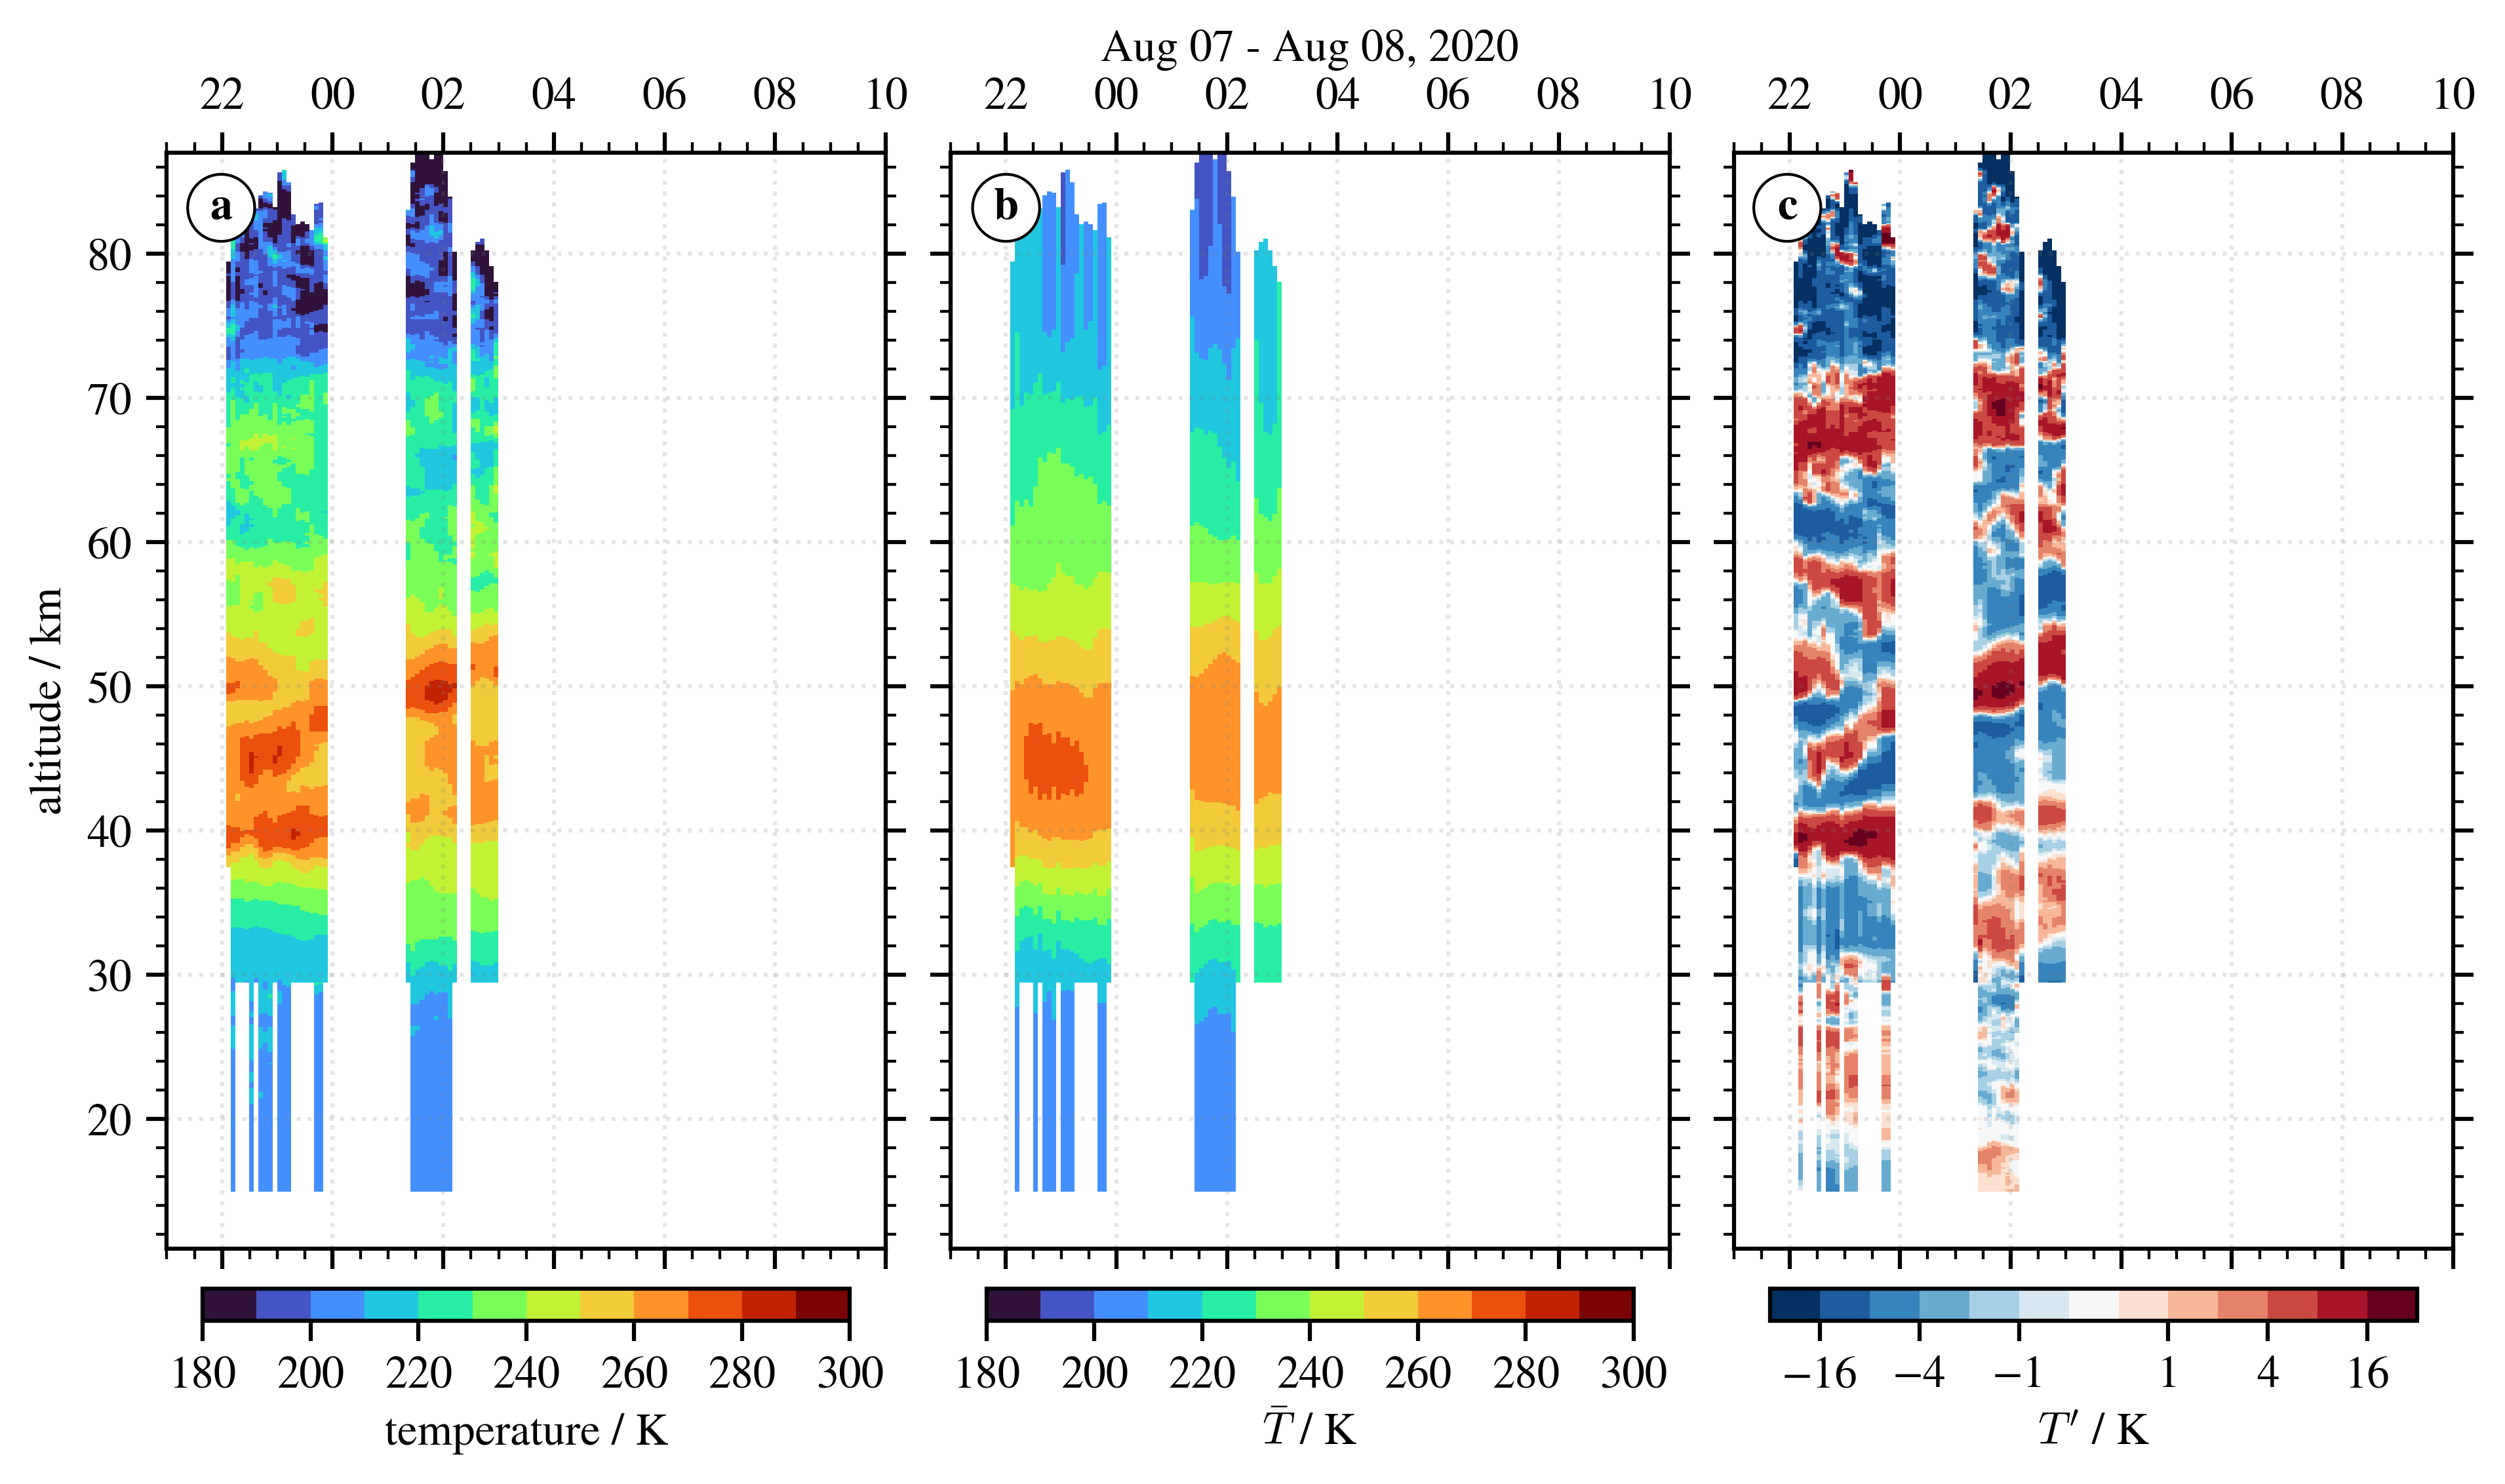
\includegraphics[width=0.99\textwidth]{figures_lidar/coral_event_20200807.png}
    \caption{}
    % \label{fig:waveletAna_dudy}
\end{figure*}


\begin{figure*}[tbp]
    \centering
    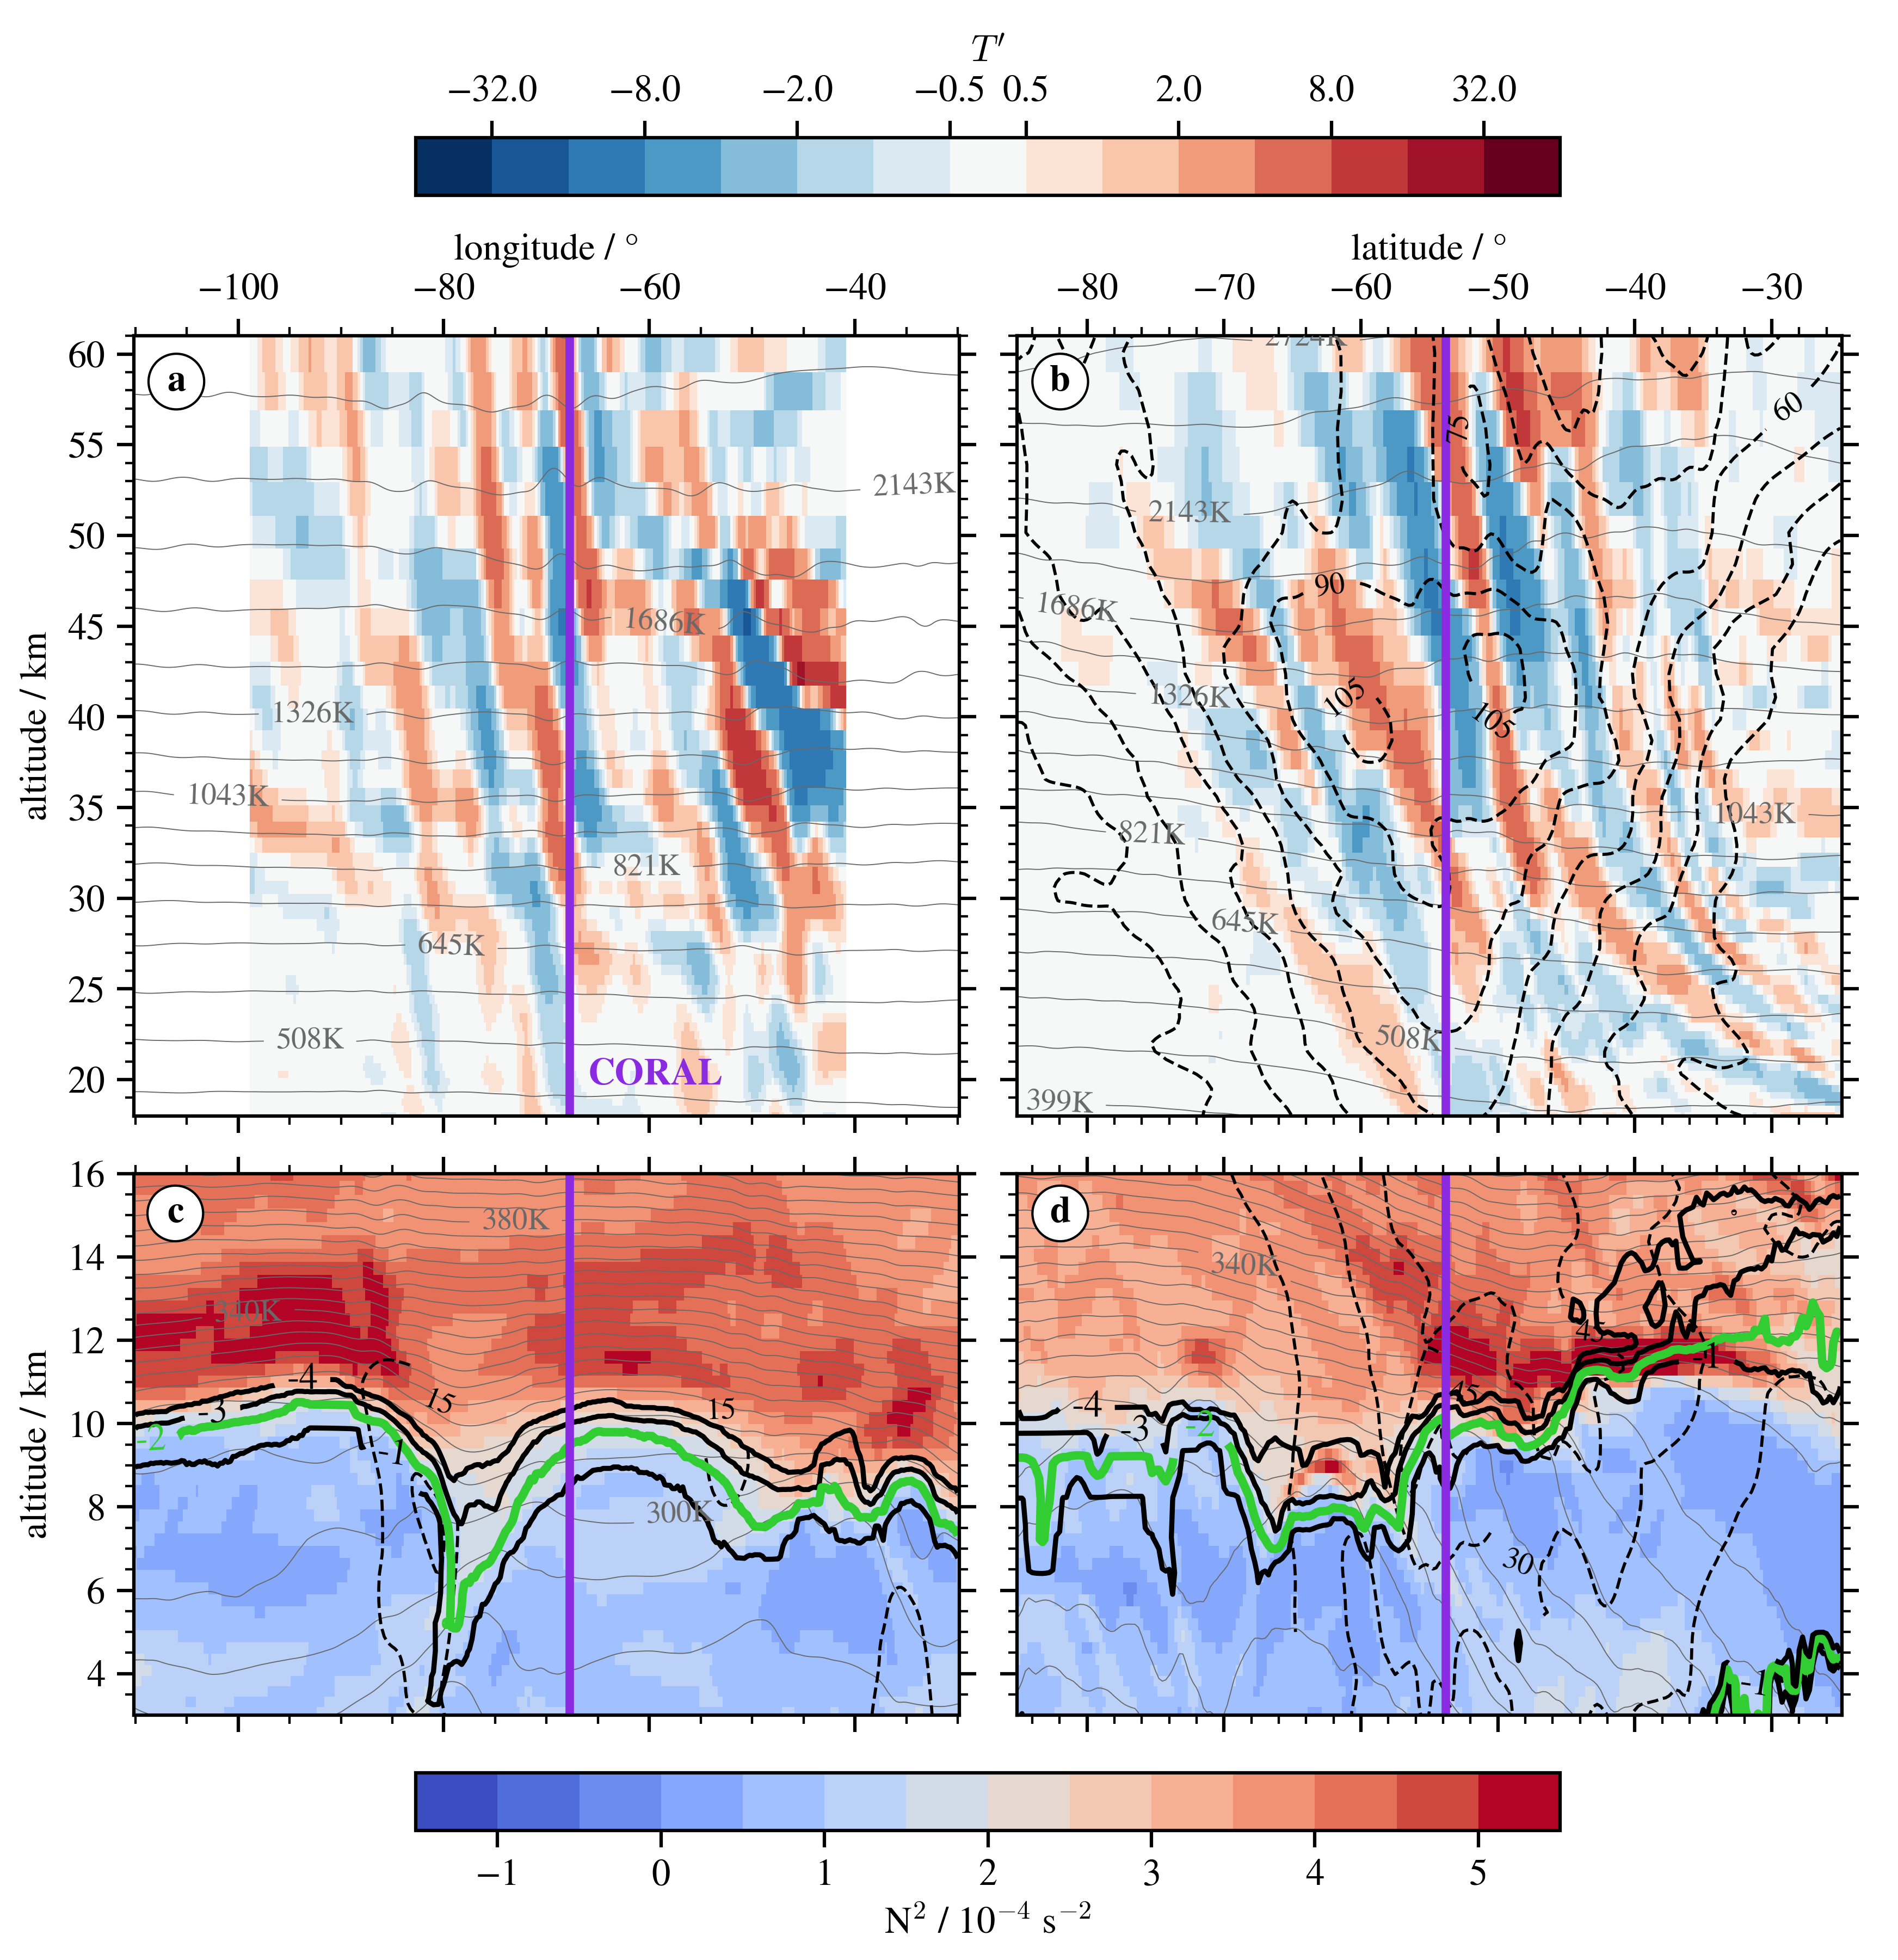
\includegraphics[width=0.99\textwidth]{figures_lidar/era5_trop_strat_2.png}
    \caption{Vertical cross sections of the stratosphere along 57.75°S (a) and 67°E (b)}
    % \label{fig:waveletAna_dudy}
\end{figure*}

\newpage
\thispagestyle{plain}

% ==== CONCLUSIONS =============================================================
% ---- set some counters to zero:
\setcounter{equation}{0}
\setcounter{table}{0}
\setcounter{figure}{0}
% ---- include tex-file:
\chapter{Conclusion}

% Answer research questions from input!!

- blabediblub


\chapter{Outlook}

- blablabla


\newpage
\thispagestyle{plain}


% ==== APPENDIX ================================================================
% ---- start appendix:
\appendix
% ---- set some counters to zero:
\setcounter{equation}{0}
\setcounter{table}{0}
\setcounter{figure}{0}
% ---- include tex-file:
\chapter{Large Quantities of Data}\label{appA}
\thispagestyle{plain}

Large quantities of data should be placed in an appendix. They should only be
``summarized'' in the chapter Results. Another way is to present
some representative cases together with some extreme cases in the chapter
Results. In any case, there should always appear a reference to the appendix in
the main part of the thesis.

\newpage
\thispagestyle{plain}


% ==== START BACK MATTER (this has no visual effect)============================
\backmatter 

% ==== BIBLIOGRAPHY ============================================================
\printbibliography
% \addcontentsline{toc}{chapter}{Bibliography}
% ---- use AMS reference format (use file ametsoc.bst included in ...
%      ... http://www.ametsoc.org/pubs/journals/AMS_Latex_V3.0.tar.gz):s
% \bibliographystyle{./ametsoc}   % ametsoc.bst in local directory
% ---- use BibTeX database file:
% \bibliography{./refs}      % mybibfile.bib in local directory
\newpage
\thispagestyle{plain}


% ==== ACKNOWLEDGMENTS =========================================================
% ---- include tex-file:
\chapter*{Acknowledgments}
\addcontentsline{toc}{chapter}{Acknowledgments}
\thispagestyle{plain}

Huge thank you to Alex and Andreas for their help and patience!

Thank you waves for making our world more interesting and fun.

% Now it is time to thank all people who have contributed to your work and who
% have supported you during your study. Do not forget to mention all relevant data
% providers and funding agencies (also provide the grant numbers).

\newpage
\thispagestyle{plain}


% ==== CURRICULUM VITAE ========================================================
% ---- include tex-file:
% \include{curricv}
% \newpage
% \thispagestyle{plain}


% ==== EPILOGUE ================================================================
% ---- include tex-file:
% \chapter*{Epilogue}
\addcontentsline{toc}{chapter}{Epilogue}
\thispagestyle{plain}


"Waves are inspiring not because they rise and fall, But because each time they fall they never fail to rise again as Ralph Waldo Emerson has so rightly said" (Ralph Waldo Emerson)

% "Sometimes, you just have to go with the waves."

% Surfing – experience sea, sky (wind), and land(coasts and breaks) at their point of convergence

% "Feelings are much like waves: we can't stop them from coming, but we can choose which one to surf."
% Jonatan Mårtensson

% "If you want the ultimate, you gotta be willing to pay the ultimate prize. It's not tragic dying doing what you love"

% "Home is where the waves are."

% "You can't stop the waves, but you can learn to surf."
% Jon Kabat-Zinn

% "Life is a wave, which in no two consecutive moments of its existence is composed of the same particles."
% John Tyndall

% Waves are inspiring not because they rise and fail, but because each time they fall. They never fail to rise again.” – Josh Billings

% Waves are inspiring not because they rise and fall, But because each time they fall they never fail to rise again as Ralph Waldo Emerson has so rightly said.

% Here is the place where you may want to tell a little story or a fairy tale
% which has some relevance for your thesis, such as ``Once upon a time, \dots''.
% The Epilogue is optional.

% \newpage
% \thispagestyle{plain}


\end{document}
% ==== END OF BODY =============================================================
